\chapter{\label{ch:2-gb-method}A method to find ghost populations using genome-wide genealogies}

\minitoc

\section{Chapter overview}
In this chapter, we introduce GhostBuster, a novel method for detecting admixture events by analyzing genome-wide genealogies inferred from genomic variation data. GhostBuster employs a mixture model to probabilistically cluster regions of the genome, identifying distinct ``types'' of coalescence histories for a target individual, with each ancestry type characterized by its coalescence rates to reference populations. Using an efficient expectation-maximization (EM) algorithm, the method iteratively updates these coalescence rates and the local ancestry of the target individual. The algorithm operates in two iterative steps. In the first step, GhostBuster assigns each genomic region of the target individual to an ancestry type based on coalescence rates to reference populations, effectively decoding local ancestry (see Figure~\ref{fig:gb-simplified-overview}A). In the second step, it refines the coalescence rates that define each ancestry by leveraging the updated local ancestry information, analogous to updating cluster means and covariances in Gaussian mixture models (see Figure~\ref{fig:gb-simplified-overview}B).

We begin by presenting the theoretical framework underlying GhostBuster in Section \ref{sec:ch2-gb-theory}, where we employ coalescent theory to model the observed genealogies. Next, in Section \ref{sec:ch2-gb-method}, we delve into the algorithmic and methodological details of the method. In Section \ref{sec:ch2-gb-data}, we discuss the various modern and ancient DNA resources used in the analyses and the construction of genealogies. In Section \ref{sec:ch2-gb-sim}, we apply GhostBuster to two simulated scenarios, demonstrating its ability to recover ghost admixture events and exploring different aspects of the method.In Section \ref{sec:ch2-gb-real}, we apply GhostBuster to real data, replicating several well-established admixture signals and comparing local ancestry estimates to prior studies. Finally, in Section \ref{sec:ch2-gb-real-eur}, we apply GhostBuster to decompose and interpret admixture events over the last 10,000 years in Europe, a period that has gained new clarity through the availability of ancient DNA.

% a figure showing the iteration between inferring coal. rates and inferring local ancestry

\begin{figure}[h!]
    \centering
    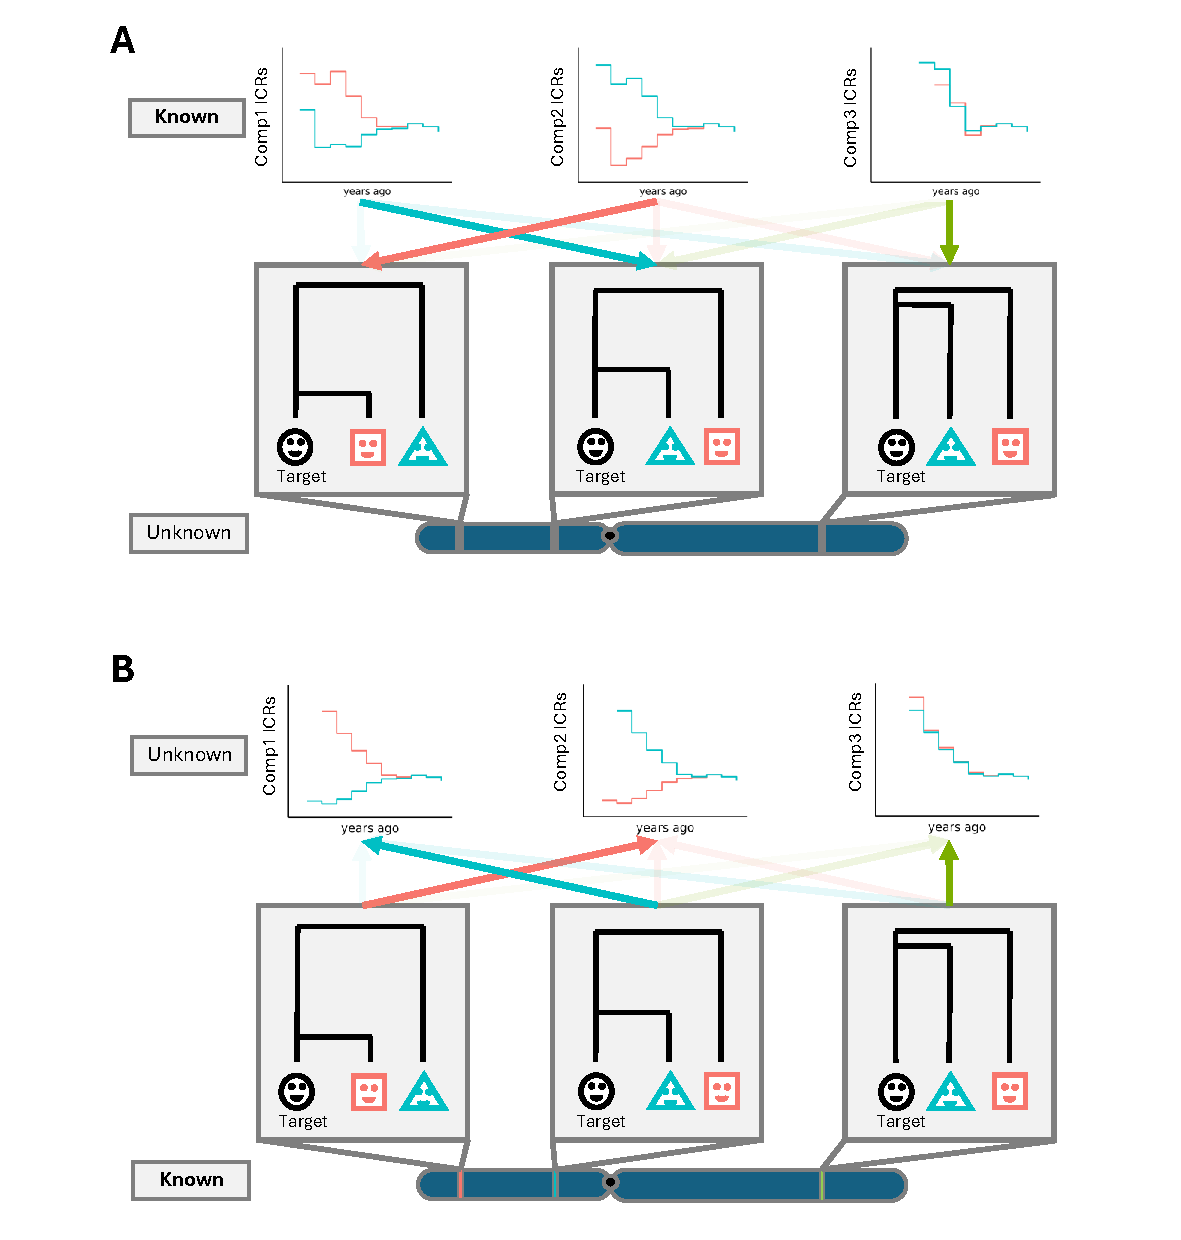
\includegraphics[width=\textwidth]{figures/thesis_gb_simplified_overview.pdf}
    \caption{\textbf{A simplified overview of GhostBuster.} GhostBuster implements an iterative expectation-maximization (EM) algorithm which cycles between two states A and B. (A) inferring local ancestry of a target individual given multiple coalescence rates of the target individuals with a set of reference populations. (B) using the local ancestry to refine the estimates of coalescence rates of target individual and the reference populations.}
    \label{fig:gb-simplified-overview}
\end{figure}

\section{Theoretical framework for our method}
\label{sec:ch2-gb-theory}

\subsection{Introduction to mixture models}
\label{sec:gb_intro_mixture_models}

Mixture models are probabilistic models that represent subpopulations within a larger population by assuming the data is generated from a mixture of distributions, each corresponding to a subpopulation or cluster.

\subsubsection{Gaussian mixture models}

One of the simplest and most widely used mixture models is the Gaussian Mixture Model (GMM). The GMM assumes that the data is generated from a mixture of multiple Gaussian distributions, where each observation is drawn from one of the Gaussian components. 

Consider a dataset $x = (x_1, x_2, \ldots, x_n)$, where $x$ is a vector of $n$ independent observations. For simplicity, assume that these observations are sampled from a mixture of two Gaussian distributions. To model this mixture, we introduce a set of hidden variables $z = (z_1, z_2, \ldots, z_n)$, where each $z_i$ is a categorical variable indicating which Gaussian component generated the corresponding observation $x_i$. Specifically, $z_i = 0$ if $x_i$ is drawn from the first Gaussian component, and $z_i = 1$ if $x_i$ is drawn from the second. The conditional distribution of the random variable $X_i$, given its corresponding hidden variable $Z_i$, is defined as follows:
\begin{align}
    X_i \mid (Z_i = 0) &\sim \mathcal{N}(\mu_1, \Sigma_1), \nonumber \\
    X_i \mid (Z_i = 1) &\sim \mathcal{N}(\mu_2, \Sigma_2), \nonumber
\end{align}
where, $\mathcal{N}(\mu_1, \Sigma_1)$ and $\mathcal{N}(\mu_2, \Sigma_2)$ denote Gaussian distributions with means $\mu_1$ and $\mu_2$, and covariance matrices $\Sigma_1$ and $\Sigma_2$, respectively. Additionally, let us assume the prior probabilities of the components are given by $P(Z_i = 0) = \pi_1$ and $P(Z_i = 1) = \pi_2$, where $\pi_2 = 1 - \pi_1$.

The aim of the GMM is to estimate the parameters corresponding to the mixture of two Gaussians, namely $\theta = (\pi_1, \mu_1, \Sigma_1, \mu_2, \Sigma_2)$, by maximizing the likelihood of the observed data. However, it is important to note that the vector $z$ is a hidden variable, meaning we do not know which observation corresponds to which cluster. Consequently, we need to maximize the ``incomplete-data likelihood,'' which integrates out the hidden variable $z$:
\begin{equation}
    L(\theta; x) = \prod_{i=1}^n \Big[\pi_1 \, \mathcal{N}(x_i \mid \mu_1, \Sigma_1) + \pi_2 \, \mathcal{N}(x_i \mid \mu_2, \Sigma_2)\Big].
\end{equation}
where, $\mathcal{N}(x_i \mid \mu_j, \Sigma_j)$ represents the Gaussian probability density function for the $j$-th component, evaluated at $x_i$. Since the likelihood involves a summation inside the product, direct maximization is challenging. To address this, the Expectation-Maximization (EM) algorithm is employed \cite{dempster1977maximum}. Instead of directly maximizing the incomplete-data likelihood, the EM algorithm operates on the ``complete-data likelihood,'' which assumes knowledge of the hidden variables $z$:
\begin{align}
    L(\theta; x, z) &= \prod_{i=1}^n \prod_{j=1}^2 \Big[\pi_j \, \mathcal{N}(x_i \mid \mu_j, \Sigma_j)\Big]^{\mathds{1}(z_{i} = j)}
\label{eq:gmm_complete_data1}
\end{align}
where, $\mathds{1}(z_i = j)$ is an indicator variable that equals 1 if the observation $x_i$ belongs to component $j$, and 0 otherwise. This formulation represents the likelihood as a product and the log-likelihood as a sum over components and observations, which eventually simplifies the optimization process.
\begin{align}
    &\log L(\theta; x, z) = \sum_{i=1}^n \sum_{j=1}^2 \mathds{1}(z_{i} = j) 
    \Big[\log \pi_j + \log \mathcal{N}(x_i \mid \mu_j, \Sigma_j)\Big] \nonumber \\
    &= \sum_{i=1}^n \sum_{j=1}^2 \mathds{1}(z_{i} = j) 
    \Big[\log \pi_j - \frac{1}{2} \log |\Sigma_j| 
    - \frac{1}{2} (x_i - \mu_j)^\top \Sigma_j^{-1} (x_i - \mu_j) 
    - \frac{d}{2} \log(2\pi)\Big].
\label{eq:gmm_complete_data2}
\end{align}

The EM algorithm alternates between the E-step, where the expected values of the hidden variables $z_i$ are computed given the current parameter estimates, and the M-step, which maximizes the expected complete-data log-likelihood with respect to the parameters $\theta$. Through these iterative updates, the EM algorithm refines the parameter estimates, ultimately converging to a local maximum of the incomplete-data likelihood \cite{dempster1977maximum} (see Figure \ref{fig:gb-gmm-visualize}). The EM algorithm for GMM operates as follows: 

\begin{figure}[h!]
    \centering
    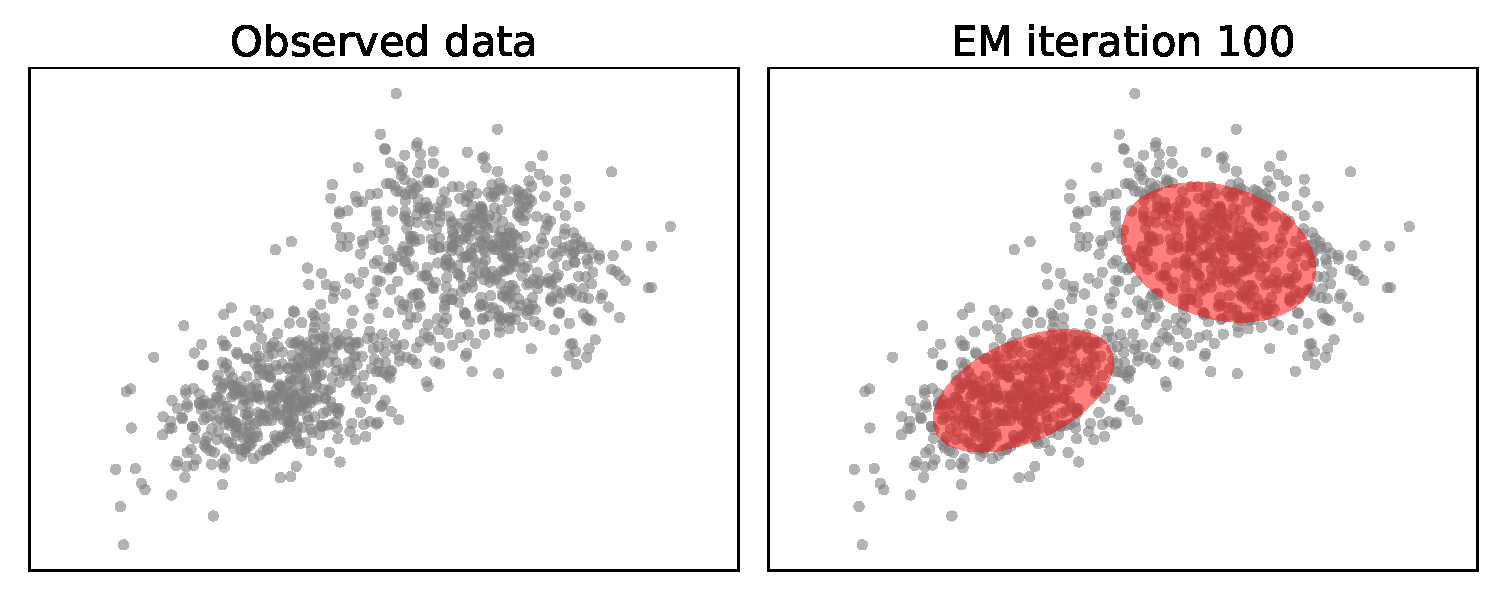
\includegraphics[width=\textwidth]{figures/gmm_visualize.pdf}
    \caption{\textbf{Gaussian mixture model.} The observed data and inferred clusters using the Gaussian mixture model after 100 EM iterations, the Gaussian mixtures inferred are represented by the red ellipse.}
    \label{fig:gb-gmm-visualize}
\end{figure}

\begin{enumerate}
    \item \textbf{E-step}: Calculates the expected log-likelihood of the complete data, given the current parameter estimates.
    \begin{align}
    &\mathbb{E}_{Z \mid X = x; \theta^{(t)}} \left[ \log L(\theta; X, Z) \right] \nonumber \\
    &= \mathbb{E}_{Z \mid X = x; \theta^{(t)}} \left[ \log \prod_{i=1}^n L(\theta; x_i, Z_i) \right] \nonumber \\
    &= \mathbb{E}_{Z \mid X = x; \theta^{(t)}} \left[ \sum_{i=1}^n \log L(\theta; x_i, Z_i) \right] \nonumber \\
    &= \sum_{i=1}^n \mathbb{E}_{Z_i \mid X_i = x_i; \theta^{(t)}} \left[ \log L(\theta; x_i, Z_i) \right] \nonumber \\
    &= \sum_{i=1}^n \sum_{j=1}^2 P(Z_i = j \mid X_i = x_i; \theta^{(t)}) \log L(\theta_j; x_i, j) \nonumber \\
    &= \sum_{i=1}^n \sum_{j=1}^2 \gamma_{j}^{(t)}(x_i) \left[ \log \tau_j - \frac{1}{2} \log |\Sigma_j| - \frac{1}{2} (x_i - \mu_j)^\top \Sigma_j^{-1} (x_i - \mu_j) - \frac{d}{2} \log(2\pi) \right]
    \end{align}
    where, the log-likelihood of the complete data comes from equation \ref{eq:gmm_complete_data2}; $\gamma_{j}(x_i)$ is the posterior probability that the data point $x_i$ was generated by the $j$-th Gaussian distribution:
    \begin{equation}
        \gamma_{j}^{(t)}(x_i) = \frac{\pi_j^{(t)} \mathcal{N}(x_i \mid \mu_j^{(t)}, \Sigma_j^{(t)})}{\sum_{j=1}^{2} \pi_j^{(t)} \mathcal{N}(x_i \mid \mu_j^{(t)}, \Sigma_j^{(t)})}
    \end{equation}
    \item \textbf{M-step}: Maximizes the expected log-likelihood, computed in the E-step, with respect to the model parameters $\theta$. For a GMM, this results in straightforward analytical update equations, as shown below:
    \begin{align}
        \pi_j^{(t+1)} &= \frac{1}{n} \sum_{i=1}^{n} \gamma_{j}^{(t)}(x_i)  \nonumber \\
        \mu_j^{(t+1)} &= \frac{\sum_{i=1}^{n} \gamma_{j}^{(t)}(x_i) x_i}{\sum_{j=1}^{n} \gamma_{j}^{(t)}(x_i)} \nonumber \\
        \Sigma_j^{(t+1)} &= \frac{\sum_{i=1}^{n} \gamma_{j}^{(t)}(x_i) (x_i - \mu_j^{t+1})(x_i - \mu_j^{t+1})^\top}{\sum_{j=1}^{n} \gamma_{j}^{(t)}(x_i)}
    \end{align}
\end{enumerate}

\subsection{Mixture model for the coalescent}
\label{the_model}
We aim to extend the basic example of mixture models to genealogies by specifically modeling coalescence events on a given target lineage as a mixture distribution. The input to our method includes, for each site, information about which individuals the target sample coalesces with and the corresponding coalescence times as we trace backwards in time. Our goal is to model this as a mixture distribution, clustering locations based on `differences' in the coalescence histories of the target lineage. The expected output of our model is a per-component coalescence rate matrix, which defines how the target individual coalesces with a set of reference populations within each specific component of the mixture.

Our method is based on the assumption that admixture can be characterized by coalescence rates with a set of reference populations. To illustrate this, consider the example of Denisovan admixture in Papuans. It is well known that Papuans carry up to 5\% Denisovan ancestry in their genomes \cite{reich2010genetic}. This archaic ancestry has different coalescence rates to reference populations compared to the majority of Papuan ancestry: regions with Denisovan ancestry exhibit more frequent coalescence events with Denisovans recently (last $100{,}000$ years), but do not tend to coalesce with modern human lineages until the time of the Denisovan-human split, estimated around $700{,}000$ years ago \cite{reich2010genetic}. Therefore, there is a clear difference in the coalescence history between archaic and non-archaic genomic regions in Papuans, which we leverage to infer admixture. Importantly, our method does not require explicit source groups or unadmixed outgroups to infer an admixture event. In the Papuan example, Denisovan ancestry not only exhibits quicker coalescence with Denisovans but also shows slower coalescence with other Papuans and modern human groups. We can leverage these differences in coalescence rates with modern human groups alone to characterize the admixture, enabling us to infer admixture without relying on explicit source groups or additional assumptions about outgroups.

Our approach begins with the need for a probabilistic model to compute the likelihood of a target lineage coalescing with reference lineages as we move backward in time. As demonstrated in Section~\ref{sec:ch1-gb-theory}, the properties of the coalescent provide a closed-form solution for the Maximum Likelihood Estimate (MLE) of coalescence rates when only two lineages are considered. When dealing with multiple lineages, the target lineage may coalesce with lineages whose descendants originate from a mixture of populations. Computing the likelihood for coalescences involving such mixed lineages is not straightforward. 

In this work, we extend the coalescent framework to address scenarios where a target lineage coalesces with a lineage that has multiple descendants, potentially belonging to several different populations. To compute the likelihood of observing coalescence events with multiple lineages, we develop a model that conditions on the inferred tree topology at each genomic site. In our model, we assume that the coalescence rate with such a lineage is proportional to the weighted sum of the coalescence rates of its descendants, as inferred from the tree at that site (see Figure~\ref{fig1} for an example). This approach is equivalent to randomly sampling a descendant and computing the pairwise likelihood, allowing us to apply the previously developed framework from Section~\ref{sec:ch1-gb-theory}. It is important to note that a simpler approach based on composite likelihood, which assumes pairwise independence between lineages, does not condition on the inferred tree topology. Such an approach would likely result in reduced statistical power.

\begin{figure}[h!]
    \centering
    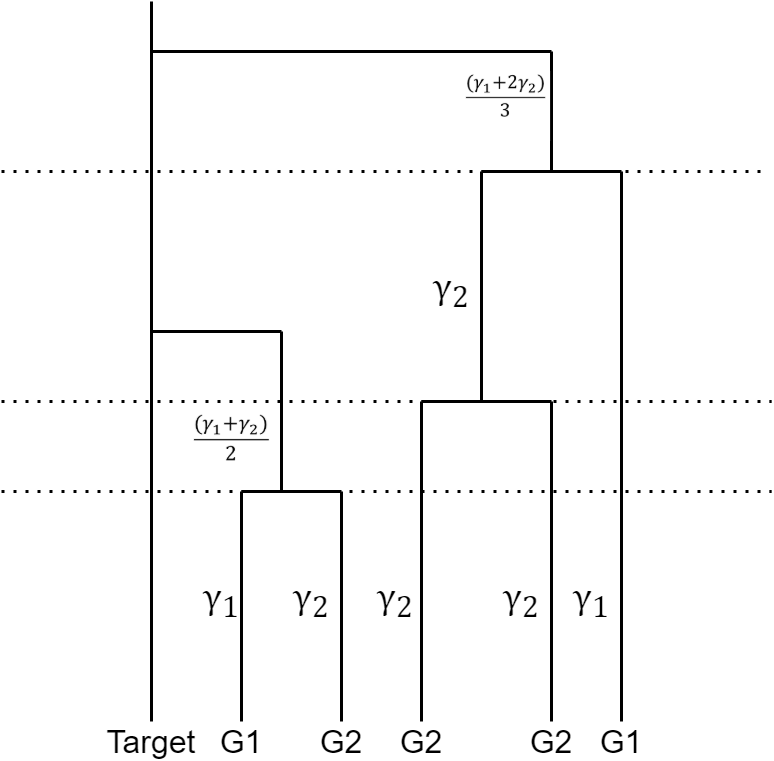
\includegraphics[scale=0.275]{figures/ghost buster simon myers-Page-1.png}
    \caption{\textbf{Toy example showing how coalescence rates depends on the weighted sum of coalescence rates of the descendants.} $\gamma_1$ and $\gamma_2$ represent coalescence rates of two populations, G1 and G2 with the target lineage.}
    \label{fig1}
\end{figure}

The MLE of coalescence rates derived in Section \ref{sec:ch1-gb-theory} also assumes independence of trees along the genome. To address this, we employ a Hidden Markov Model (HMM) to capture ancestry switches along the genome, treating each location as Markovian. This approach mitigates the independence assumption and further enhances the power of our likelihood estimation.

\subsubsection{Likelihood of a single coalescence event}
Under our model, we derive the likelihood of a single coalescence event involving a lineage whose descendants are drawn from a mixture of populations. Let the coalescing clade or lineage have $n_g$ descendants from population $g$, with the total number of descendants given by $\sum_{g=1}^R n_g$. The probability distribution for observing a coalescence event at time $t$, given the matrix of coalescence rates per group per epoch $\gamma$, is expressed as:
\begin{equation}
    P(t \mid \gamma) = \frac{\sum_{g=1}^R \gamma_g(m) n_g}{\sum_{g=1}^R n_g} 
    e^{-\sum_{g=1}^R \gamma_g \cdot O_g(t)},
\label{eq:gb_single_coal_like}
\end{equation}
where, $n_g$ is the number of descendants in group $g$, $\gamma_g(m)$ is the coalescence rate of group $g$ during epoch $m$, and $O_g(t)$ is the opportunity, defined as the sum of branch lengths from the previous coalescence time to $t$ for all group $g$ individuals.

This weighting is equivalent to randomly sampling a descendant from the coalescing lineage, with the probability determined by its coalescence rate with the target individual. Specifically, let \( q \) be a categorical random variable that indicates which individual coalesces with the target. The probability of selecting the \( k \)-th descendant is given by:
\begin{align}
    P(q = k \mid \gamma) = \frac{\gamma_{g(k)}(m)}{\sum_{g=1}^R \gamma_g(m)},
\end{align}
where, \( g(k) \) denotes the population to which the \( k \)-th descendant belongs. 

The joint probability of observing a coalescence event at time \( t \) and the descendant \( q = k \), assuming conditional independence between \( t \) and \( q \), can be expressed as:
\begin{align}
    P(t, q = k \mid \gamma) &= P(t \mid q = k, \gamma) P(q = k \mid \gamma) \nonumber \\
    &= P(t \mid \gamma) P(q = k \mid \gamma) \nonumber \\
    &= \left( \frac{\sum_{g=1}^R \gamma_g(m) n_g}{\sum_{g=1}^R n_g} 
    e^{-\sum_{g=1}^R \gamma_g \cdot O_g(t)} \right)
    \frac{\gamma_{g(k)}(m)}{\sum_{g=1}^R \gamma_g(m)} \nonumber \\
    &= \frac{\gamma_{g(k)}(m)}{\sum_{g=1}^R n_g} 
    e^{-\sum_{g=1}^R \gamma_g \cdot O_g(t)}.
\end{align}

\subsection{EM derivation: the likelihood}
\subsubsection{Terminology}
\label{terminology}
We aim to fit a mixture model to cluster the genome based on variations in coalescence rates. To reduce computational costs, we divide the genome into $T$ small grids and focus on inferring local ancestry at these grid points, rather than at every individual location on the genome (by default, grid points are equally spaced $10$kb apart). Additionally, we approximate coalescence rates as piecewise constant functions over time, defined by $E$ time epochs that are equally spaced on a logarithmic scale \cite{schiffels2014inferring}. For the derivation of the EM algorithm, we use the following terminology:
\begin{itemize}    
    \item Our input data are the genealogies which contain:
    \begin{enumerate}
        \item $t_{li} =$ Coalescence time for the $i^{th}$ coalescence event (measured from the previous coalescence event) in the $l^{th}$ grid
        \item $n_{lig} =$ The number of group $g$ individuals coalescing in the $i^{th}$ coalescence event and the $l^{th}$ grid
        \item $Q_l =$ Number of coalescence events between the target lineage and reference samples corresponding to the tree at $l^{th}$ grid along the genome.
        \item $e_{li} =$ Epoch in which the $i^{th}$ coalescence event happens in the $l^{th}$ grid
        \item $r_{l} =$ Genetic distance between the $(l-1)^{th}$ and $l^{th}$ position along the genome
    \end{enumerate}

    \item The parameters we infer using the EM algorithm are:
    \begin{enumerate}
        \item $\gamma_{jg}(m) =$ Coalescence rate between reference group $g$ and the target in the $j^{th}$ mixture component and in epoch $m$
        \item $\pi_j = P(z_l = j) =$ Cluster proportion of the $j^{th}$ mixture component
        \item $\lambda =$ Admixture time in generations
    \end{enumerate}

    \item Let us define some fixed constants we will use in the derivation:
    \begin{enumerate}
        \item $C =$ Total number of coalescence events between the target lineage and reference samples across the whole genome
        \item $T =$ Total number of grid points
        \item $A =$ Number of clusters assumed in the target
        \item $N_{li} =$ Number of reference individuals subtending the $i^{th}$ lineage with which the target lineage coalesces in the $i^{th}$ coalescence event and the $l^{th}$ grid
        \item $E =$ Number of time epochs where the coalescence rates are assumed piecewise constant (by default, we have $20$ time epochs)
    \end{enumerate}

    \item We will maintain consistency by using the same subscript to index the same variables throughout the derivation:
    \begin{enumerate}
        \item $l =$ Grid position along the genome
        \item $i =$ Coalescence event count
        \item $g =$ Predefined reference groups (example: Papuans, Denisovans, etc.)
        \item $j =$ Cluster or component in the mixture
        \item $e =$ Time epoch going backwards in time
    \end{enumerate}

    \item In the E-step, we introduce hidden variables to facilitate analytical updates. These variables are probabilistically inferred based on the current estimates of the parameters:
    \begin{enumerate}
        \item $z_l =$ Local ancestry of the target at position $l$
        \item $q_{li} =$ Reference individual index that coalesces in the $i^{th}$ coalescence event and the $l^{th}$ grid
        \item $\omega_l =$ Number of recombinations since admixture between positions $l-1$ and $l$
    \end{enumerate}
\end{itemize}


\subsubsection{The ``true'' likelihood}
We aim to formalize the likelihood for the mixture model described in Section \ref{the_model}. Following the approach of the EM algorithm for GMMs outlined in Section \ref{sec:gb_intro_mixture_models}, we first define the ``incomplete-data likelihood,'' which assumes access to only the directly observable quantities. This includes: (1) The vector of coalescence time for each event between the target lineage and reference samples, denoted as $t = (t_1, t_2, \ldots, t_C)$. (2) The corresponding time epoch vector, $e = (e_1, e_2, \ldots, e_C)$. (3) The corresponding clade distribution vector, $n_g = (n_{g,1}, n_{g,2}, \ldots, n_{g,C})$, which records the number of group $g$ individual corresponding to a coalescence event. 

The incomplete-data likelihood is given as follows: 
\begin{align}
    P(t \mid \gamma, \pi, \lambda) = \sum_{z} P(t \mid z, \gamma, \pi, \lambda) P(z \mid \gamma, \pi, \lambda) 
\end{align}
where, $z$ is the hidden categorical random variable which dictates the ``type'' of coalescence history for the target individual. We characterize these different types of coalescence history by the different coalescence rates between the target individual and reference samples. $\gamma, \pi, \lambda$ are the set of parameters to be inferred; $\gamma$ is the coalescence rate matrix, $\pi$ are the mixture proportions, and $\lambda$ is the admixture time. $\sum_{z}$ sums over all possible configurations of this hidden variable in order to obtain the incomplete-data likelihood. It is important to note given this hidden variable $z$ the conditional probability $P(t \mid z, \gamma, \pi, \lambda)$ can be factorized over coalescence events. 
\begin{align}
    P(t \mid \gamma, \pi, \lambda) = \sum_{z} \prod_{c=1}^C P(t_c \mid z_c, \gamma, \pi, \lambda) P(z \mid \gamma, \pi, \lambda) 
\end{align}

We can now utilize our model as described in Section \ref{the_model} and equation \ref{eq:gb_single_coal_like} to get $P(t_c \mid z_c,\gamma, \pi, \lambda)$:
\begin{align}
    P(t \mid \gamma, \pi, \lambda) = \sum_{z} \left( \prod_{c=1}^C \frac{\sum_{g=1}^R \gamma_{jg}(e_c) n_{g}}{\sum_{g=1}^R n_{g}} e^{-\sum_{g=1}^R \gamma_{jg} \cdot O_{g} (t)} \right) P(z \mid \gamma, \pi, \lambda) 
\label{eq:gb_incomplete_data_likelihood}
\end{align}

As with the GMM, the incomplete-data likelihood in equation \ref{eq:gb_incomplete_data_likelihood} is not directly optimizable due to its complex form. To address this, we employ the EM algorithm, which utilizes the complete-data likelihood to maximize the incomplete-data likelihood. This assumes access to complete information, including both observable quantities and hidden variables. In our case, hidden variables to facilitate computations in the EM algorithm include: (1) \( z = (z_1, z_2, \ldots, z_C) \), which records the mixture component assignment for the \( c^{th} \) coalescence event. (2) \( q = (q_1, q_2, \ldots, q_C) \), which identifies the reference individual involved in the \( c^{th} \) coalescence event. (3) $\omega = (\omega_l)$, which identifies number of recombination events since admixture between positions $l-1$ and $l$. 

The complete-data likelihood represents the joint probability of observing the coalescence times \( t \), along with the hidden variables \( z \) and \( q \), given the model parameters \( \gamma \), \( \pi \), and \( \lambda \). We express this likelihood as the product of probabilities for each coalescence event, summed across all coalescence events \( c \), clusters \( j \), reference populations \( g \), and time epochs \( m \) in the ancestral recombination graph (ARG):
\begin{equation}
    P (t,z,q \vert \gamma, \pi, \lambda) = \prod_{c=1}^{C} \prod_{j = 1}^A \prod_{g =1}^{R} \prod_{m = 1}^E P (t_c,z_c = j,q_c=g \vert \gamma, \pi, \lambda)^{\mathds{1}_{\{z_c = j\}} \mathds{1}_{\{q_c = g\}} \mathds{1}_{\{e_c = m\}}}
\label{true_likelihood1}
\end{equation}

Here, \( t \) represents the vector of observed coalescence times, while \( z \) and \( q \) are hidden variables for each coalescence event. The indicator functions \( \mathds{1}_{\{z_c = j\}} \), \( \mathds{1}_{\{q_c = g\}} \), and \( \mathds{1}_{\{e_c = m\}} \) ensure that the probability contributions are assigned to the appropriate cluster, reference population, and time epoch. 

Similar to GMM we will employ the EM algorithm, where the E-step computes the posterior distribution of the hidden variables given the observed data and the current model parameters, while the M-step maximizes the expected complete-data log-likelihood with respect to the model parameters \( \gamma \), \( \pi \), and \( \lambda \). 


It is important to note we are currently assuming conditional independence of coalescence time given the hidden variables. $z_c$ will be replaced in future.  

that coalescence events in an ARG can span more than one tree, particularly for nodes lower in the tree, which are less likely to be affected by recombination and thus persist longer along the genome. Next, we introduce windowing the genome and appropriately scaling the likelihood to still obtain the above equation as follows:
\begin{equation}
    \footnotesize
    P(t,z,q \vert \gamma, \pi, \lambda) = \prod_{c=1}^{C} \prod_{j = 1}^A \prod_{g =1}^{R} \prod_{m = 1}^E \prod_{l =1}^{T} \left( P(t_c,z_c = j,q_c=g \vert \gamma, \pi, \lambda)^{\mathds{1}_{\{z_c = j\}} \mathds{1}_{\{q_c = g\}} \mathds{1}_{\{e_c = m\}}} \right) ^{\frac{\mathds{1}_{\{w_c = l\}}}{K_c}}
\label{true_likelihood2}
\end{equation}
where, $\mathds{1}_{\{w_c = l\}}$ is the indicator random variable indicating if the $l^{th}$ grid point overlaps with the node corresponding to the $c^{th}$ coalescence event, and $K_c$ is the total number of grids the node corresponding to the $c^{th}$ coalescence event spans (referred to as node persistence). We scale the likelihood in equation \ref{true_likelihood2} by $\frac{1}{K_c}$ so that once multiplied over windows it remains equal to the original likelihood in equation \ref{true_likelihood1}. More details about the calculation of node persistence can be found in Section \ref{sec:ch2-gb-node-persistence}.

\subsubsection{Accounting for uncertain coalescence events}

Genealogies inferred from genetic variation data come with the added complexity of uncertainty, as they are not always entirely accurate. The support for a particular node in the tree is stronger when there is a mutation mapped just above that node. To account for this uncertainty, we scale the likelihood by the confidence in each coalescence event. Specifically, as we move backward in time along the target lineage, we count the number of coalescence events that occur before encountering a mutation. All coalescence events between successive mutations are then weighted based on the number of such events. This adjustment is ad hoc, but improves the robustness of our method to errors in inferred genealogies, as demonstrated in empirical analyses. Overall, this results in scaling the likelihood in equation \ref{true_likelihood2} by an additional term, $H_c$, which calculates the effective contribution of a coalescence event to the likelihood depending on its certainty. The updated likelihood is now given as:
\begin{equation}
    \footnotesize
    P(t,z,q \vert \gamma, \pi, \lambda) = \prod_{c=1}^{C} \prod_{j = 1}^A \prod_{g =1}^{R} \prod_{m = 1}^E \prod_{l =1}^{T} \left( P(t_c,z_c = j,q_c=g \vert \gamma, \pi, \lambda)^{\mathds{1}_{\{z_c = j\}} \mathds{1}_{\{q_c = g\}} \mathds{1}_{\{e_c = m\}}} \right) ^{\frac{\mathds{1}_{\{w_c = l\}}}{B_c}}
\label{true_likelihood3}
\end{equation}
where, $B_c = H_cK_c$ is the effective scaling factor accounting for node persistence and certainty of coalescence events in inferred genealogies. More details about calculation of this weighting can be found in section \ref{sec:ch2-gb-uncertain-coal}.

Although we divide the likelihood in different grids it is not straight-forward to optimize the likelihood directly. In the next section, we approximate the likelihood in equation \ref{true_likelihood3} so that we can use Markov models for inference. 

\subsubsection{Markovian approximation to the ``true'' likelihood}
% We perform a Markovian approximation to the ``true'' likelihood defined in equation \ref{true_likelihood3} and re-write the cluster membership $z$ in terms of window $l$ instead of coalescence event $c$. More formally we approximate as follows:
% \begin{equation}
%     P (t,z,q \vert \gamma, \pi, \lambda) \approx \prod_{l =1}^{T} \prod_{j = 1}^A \prod_{i = 1}^{Q_l} \prod_{k =1}^{N_{li}} \prod_{m = 1}^E \Big( P(t_{li}, q_{li} = k, z_l = j \vert \gamma, \pi, \lambda) ^ {\mathds{1}_{\{q_{l i} = k\}}  \mathds{1}_{\{e_{l i} = m\}}} \Big) ^{\frac{\mathds{1}_{\{z_l = j\}}}{B_{li}}}
%     \label{markov_approx}
% \end{equation}

We begin by approximating the likelihood of the true model defined in Equation \ref{true_likelihood3} by transitioning from coalescence event-level indexing \( c \) to genomic position based indexing \( l \). The approximate likelihood we optimize can be written as:

\begin{equation}
    P(t \vert \gamma, \pi, \lambda) \approx \prod_{l=1}^{T} \prod_{j = 1}^A \prod_{i=1}^{Q_l} \prod_{m=1}^{E} P(t_{li} \vert z_l = j, \gamma, \pi, \lambda)^{\frac{\mathds{1}_{\{e_{l i} = m\}}\mathds{1}_{\{z_l = j\}}}{B_{li}}}
    \label{approx_likelihood_start}
\end{equation}
where \( z_l \) represents the cluster membership (local ancestry) assignment for position \( l \), \( t_{li} \) represents the observed coalescence times for the \( i^{th} \) event overlapping grid point \( l \), \( Q_l \) is the total number of coalescence events at position $l$, and \( B_{li} \) normalizes the contributions of coalescence events across windows. This window-based approximation simplifies the likelihood by replacing coalescence event-level specificity with genomic position-level aggregation, while explicitly conditioning on \( z_l \).

To facilitate the expectation-maximization (EM) algorithm, we introduce the hidden variable \( q_{li} \), which records the reference individual involved in the \( i^{th} \) coalescence event at window \( l \). While \( q_{li} \) is not directly included in the observed likelihood, it is useful for intermediate computations. The full likelihood incorporating \( q_{li} \) for the purpose of EM can be written as:
\begin{equation}
    P (t,z,q \vert \gamma, \pi, \lambda) \approx \prod_{l =1}^{T} \prod_{j = 1}^A \prod_{i = 1}^{Q_l} \prod_{k =1}^{N_{li}} \prod_{m = 1}^E \Big( P(t_{li}, q_{li} = k, z_l = j \vert \gamma, \pi, \lambda) ^ {\mathds{1}_{\{q_{l i} = k\}}  \mathds{1}_{\{e_{l i} = m\}}} \Big) ^{\frac{\mathds{1}_{\{z_l = j\}}}{B_{li}}}
    \label{markov_approx}
\end{equation}

Here, \( q_{li} \) facilitates the summation required in the E-step, where we compute the posterior probabilities of \( q_{li} \) given \( t_{li} \) and \( z_l \). Importantly, introducing \( q_{li} \) does not alter the likelihood, as summing over \( q_{li} \) recovers the same rate as the formulation without \( q_{li} \). The true approximation lies in transitioning from \( z_c \) (coalescence event-level cluster membership) to \( z_l \) (window-level cluster membership), which simplifies computations and enables the use of Markovian models like HMMs for inference. By separating the dependence on \( z_l \) and \( q_{li} \), we maintain interpretability of \( z_l \) as local ancestry at position \( l \), while using \( q_{li} \) purely as an auxiliary variable for computational efficiency in the EM framework. We further simplify the equation \ref{markov_approx} and separate it into two parts.

\begin{equation}
    \footnotesize
    P (t,z,q \vert \gamma, \pi, \lambda) = \underbrace{P(z \vert \pi, \lambda)}_{\text{Term 2}} \prod_{l =1}^{T} \prod_{j = 1}^A \prod_{i = 1}^{Q_l} \prod_{k =1}^{N_{li}} \prod_{m = 1}^E \underbrace{\Big( P(t_{li}, q_{li} = k \vert z_l = j, \gamma) ^ {\mathds{1}_{\{q_{l i} = k\}}  \mathds{1}_{\{e_{l i} = m\}}} \Big) ^{\frac{\mathds{1}_{\{z_l = j\}}}{B_{li}}}}_{\text{Term 1}}
    \label{eq:term1_term2}
\end{equation}

We perform expectation-maximization and optimize term 1 to get the $\gamma$ (coalescence rates) and term 2 to get $\lambda$ (admixture time) and $\pi$ (global cluster proportions). In the following sections we simplify our calculations by deriving the EM updates for term 1 and term 2 separately. 

\subsection{EM derivation: terminology}


\subsection{EM derivation: inference of coalescence rates}
We write the likelihood term 1 in equation \ref{eq:term1_term2} which only depends on coalescence rates as follows: 
\begin{equation}
     P(t, q \vert z, \gamma) = \prod_{l = 1}^T \prod_{j = 1}^A \prod_{i = 1}^{Q_l} \prod_{k =1}^{N_{li}} \prod_{m = 1}^E   P(t_{li}, q_{l i} = k \vert z_l = j, \gamma) ^ {\frac{\mathds{1}_{\{z_l = j\}}\mathds{1}_{\{q_{l i} = k\}}  \mathds{1}_{\{e_{l i} = m\}}}{B_{li}}}
\label{eq:scaled_ll}
\end{equation}
where, the indicator random variables $\mathds{1}_{\{z_l = j\}}$, $\mathds{1}_{\{e_{l i} = m\}}$ and, $\mathds{1}_{\{q_{l i} = k\}}$ are present to simplify the equation when writing it down for all the trees and coalescence events in that tree. The log-likelihood is given by:

\begin{equation}
     \log P(t, z, q \vert \gamma) = \sum_{l = 1}^T \sum_{j = 1}^A \sum_{i = 1}^{Q_l} \sum_{k =1}^{N_{li}} \sum_{m = 1}^E  \frac{\mathds{1}_{\{q_{l i} = k\}} \mathds{1}_{\{z_l = j\}} \mathds{1}_{\{e_{l i} = m\}} \log P(t_{li}, q_{l i} = k \vert z_l = j, \gamma)}{B_{li}} 
\end{equation}

We can simplify the log-likelihood further as:
\begin{equation}
    P(t_{li}, q_{li} = k | z_l = j, \gamma ) = P(t_{li} | \gamma, z_l = j, q_{li} = k)P(q_{li} = k | z_l = j, \gamma)
\end{equation}

\begin{enumerate}
\item Looking at the first term, $P(t_{li} \mid \gamma, z_l = j, q_{li} = k)$, which represents the probability of coalescing at time $t_{li}$, conditioned on the reference individual with which the target coalesces ($q_{li}$), the local ancestry of the target ($z_l$), and the coalescence rates ($\gamma$), we assume conditional independence such that:
\begin{align}
    P(t_{li} | \gamma, z_l = j, q_{li} = k) = P(t_{li} | \gamma, z_l = j) \nonumber \\
    P(t_{li} | \gamma, z_l = j) = \frac{\sum_{g=1}^R\gamma_{jg}(m)n_{lig}}{\sum_{g=1}^R n_{lig}}e^{-\sum_{g=1}^R \gamma_{jg} \cdot O_{lg}[i]}
\end{align}
where, $n_{lig} =$  number of group $g$ individuals coalescing in the $i^{th}$ coalescence event and position $l$ and, $O_{lg}[i] =$ sum of branch length from lower epoch boundary to the $i^{th}$ coalescence event corresponding to all group g individuals coalescing at $t_{li}$. This equation is derived from the likelihood for a single coalescence event as discussed in equation \ref{eq:gb_single_coal_like}.
\vspace{3mm}
\item For the second term, we assume the probability that the target coalesces with a reference individual $k$ to be directly proportional to its coalescence rate with it. More formally, $P(q_{li} = k \mid z_l = j, \gamma)$, or the probability that the target coalesces with a reference individual, conditioned on the local ancestry of the target ($z_l$) and the coalescence rates ($\gamma$) can be simplified to:
\begin{equation}
    P(q_{li} = k | z_l = j, \gamma) = \frac{\gamma_{jg(k)}(m)}{\sum_{g=1}^R \gamma_{jg}(m)n_{lig}}
\label{eq:qli}
\end{equation}

where, $g(k)$ means the group assignment (among $R$ groups) of the $k^{th}$ individual in the reference panel. 
\end{enumerate}

Overall $P(t_{li}, q_{li} = k | z_l = j, \gamma )$ can be written as (only focusing on terms depending on cluster membership $j$): 
\begin{align}
    P(t_{li}, q_{li} = k | \gamma, z_l = j ) = \frac{\gamma_{jg(k)}(m)e^{-\sum_{g=1}^R \gamma_{jg}\cdot O_{lg}[i]}}{\sum_{g=1}^R n_{lig}} \nonumber \\
    \propto \gamma_{jg(k)}(m) \times e^{-\sum_{g=1}^R \gamma_{jg}\cdot O_{lg}[i]}
    \label{eq:likelihood}
\end{align}

We can maximize the likelihood corresponding to term 1 through an expectation-maximization algorithm. In the E-step, we define the expected log-likelihood of the data given the hidden variables and the previous estimates of the parameters (including $\lambda$ and $\pi$), and in the M-step, we maximize this expected log-likelihood. Under the expectation-maximization framework, it is guaranteed that the likelihood increases with every iteration, thereby ensuring convergence to a local minimum. Next, we derive the E-step and M-step for our likelihood in equation \ref{eq:likelihood}.
 
\subsubsection{E-step}

In the E-step we calculate the expected log-likelihood, where the expectation is with respect to the hidden variables conditioned on the data and previous parameter estimation. We therefore proceed by stating the expected log-likelihood in our case:
\begin{equation}
   \mathbb{E}_{z, q | \gamma^{t-1}, \lambda^{t-1}, \pi^{t-1}, t} \Big(  \sum_{l = 1}^T \sum_{j = 1}^A \sum_{i = 1}^{Q_l} \sum_{k =1}^{N_{li}} \sum_{m = 1}^E  \frac{\mathds{1}_{\{q_{l i} = k\}} \mathds{1}_{\{z_l = j\}} \mathds{1}_{\{e_{l i} = m\}} \log P(t_{li}, q_{l i} = k \vert z_l = j, \gamma)}{B_{li}} \Big)
 \end{equation}

We start simplifying the expected log-likelihood by taking the expectation inside the summations, and transforming the expected value of indicator random variables as probabilities.  
\begin{equation}
    \footnotesize
    = \sum_{l = 1}^T \sum_{j = 1}^A  \sum_{i = 1}^{Q_l} \sum_{k =1}^{N_{li}} \sum_{m = 1}^E \mathds{1}_{\{e_{l i} = m\}} P(q_{li} = k, z_l = j \mid \gamma^{t-1}, \lambda^{t-1}, \pi^{t-1}, t) \frac{\log(P(t_{li}, q_{l i} = k \mid z_l = j, \gamma ))}{B_{li}}
\end{equation}

Simplifying further and substituting the value of $\log(P( t_{li}, q_{l i} = k  | z_l = j, \gamma ))$ from equation \ref{eq:likelihood}. Note, we omit the constants of proportionality as they do not depend on the coalescence rates and thus will not affect the maximization in the M-step.
\begin{align}
    &= \sum_{l = 1}^T \sum_{j = 1}^A \sum_{i = 1}^{Q_l} \sum_{k = 1}^{N_{li}} \sum_{m = 1}^E \Bigg( 
        P(q_{li} = k \mid \gamma^{t-1}, t, z_l = j) P(z_l = j \mid t, \gamma^{t-1}, \lambda^{t-1}, \pi^{t-1}) \nonumber \\
    &\quad \times \mathds{1}_{\{e_{l i} = m\}} \frac{\log(P(t_{li}, q_{l i} = k \mid z_l = j, \gamma))}{B_{li}} \Bigg) \nonumber \\
    &= \sum_{l = 1}^T \sum_{j = 1}^A \sum_{i = 1}^{Q_l} \sum_{k = 1}^{N_{li}} \sum_{m = 1}^E \Bigg( 
        P(q_{li} = k \mid \gamma^{t-1}, t, z_l = j) P(z_l = j \mid t, \gamma^{t-1}, \lambda^{t-1}, \pi^{t-1}) \nonumber \\
    &\quad \times \mathds{1}_{\{e_{l i} = m\}} \frac{\log(\gamma_{jg(k)}(m)) - \sum_{g=1}^R \gamma_{jg} \cdot O_{lg}[i]}{B_{li}} \Bigg) 
\end{align}

Note the probability of $q_{li}$ (as defined in equation \ref{eq:qli}) does not depend on admixture time and proportion. We can simplify the expected log-likelihood further and switch the individual assignment hidden variable $q_{li}$ to more rapidly computable group assignment hidden variable $q'_{li}$. 
\begin{align}
   &\color{red}{\sum_{l = 1}^T \sum_{j = 1}^A \sum_{i = 1}^{Q_l} \sum_{k = 1}^{N_{li}} \sum_{m = 1}^E \Bigg( 
       P(q_{li} = k \mid \gamma^{t-1}, z_l = j) P(z_l = j \mid t, \gamma^{t-1}, \lambda^{t-1}, \pi^{t-1})} \nonumber \\
   &\quad \color{red}{\times \mathds{1}_{\{e_{l i} = m\}} \frac{\log(\gamma_{jg(k)}(m))}{B_{li}} \Bigg)} \nonumber \\
   &\color{blue}{- \sum_{l = 1}^T \sum_{j = 1}^A \sum_{i = 1}^{Q_l} \sum_{k = 1}^{N_{li}} \sum_{m = 1}^E \Bigg( 
       P(q_{li} = k \mid \gamma^{t-1}, z_l = j) P(z_l = j \mid t, \gamma^{t-1}, \lambda^{t-1}, \pi^{t-1})} \nonumber \\
   &\quad \color{blue}{\times \mathds{1}_{\{e_{l i} = m\}} \frac{\sum_{g=1}^R \gamma_{jg} \cdot O_{lg}[i]}{B_{li}} \Bigg)}
\end{align}

We group the individuals based on group assignment in the first term (red term) and use $\sum_{k =1}^{N_{li}} P(q_{li} = k | \gamma^{t-1}, z_l = j) = 1$ in the second term (blue term). 
\begin{align}
   &\color{red}{\sum_{l = 1}^T \sum_{j = 1}^A \sum_{i = 1}^{Q_l} \sum_{g = 1}^{R} \sum_{m = 1}^E \Bigg( 
       P(q'_{li} = g \mid \gamma^{t-1}, z_l = j) P(z_l = j \mid t, \gamma^{t-1}, \lambda^{t-1}, \pi^{t-1})} \nonumber \\
   &\quad \color{red}{\times \mathds{1}_{\{e_{l i} = m\}} \frac{\log(\gamma_{jg}(m))}{B_{li}} \Bigg)} \nonumber \\
   &\color{blue}{- \sum_{l = 1}^T \sum_{j = 1}^A \sum_{i = 1}^{Q_l} \sum_{m = 1}^E \Bigg( 
       P(z_l = j \mid t, \gamma^{t-1}, \lambda^{t-1}, \pi^{t-1}) \mathds{1}_{\{e_{l i} = m\}}}  \sum_{g=1}^R \frac{\gamma_{jg} \cdot O_{lg}[i]}{B_{li}} \Bigg)
   \label{estep:ell-simple}
\end{align}

Let us denote $U_{l,i,g,j,m}^{t-1}$ as the first red probability, corresponding to the membership ``group g individual coalesces in the $i^{th}$ coalescence event''. And, let us denote $T_{l,j}^{t-1}$ as the first blue probability, corresponding to the local ancestry of the target. We use the forward-backward algorithm for HMMs to evaluate $T_{l,j}$ in future section \ref{sec:term2_estep}. Whereas, we calculate $U_{l,i,g,j,m}^{t-1}$ based on our assumed model that the probability of coalescing with reference individual is directly proportional to its coalescence rate and for a group of individual on the weighted mean of their individual coalescence rates (see section \ref{the_model} and figure \ref{fig1}):
\begin{equation}
    U_{l,i,g,j,m}^{t-1} = P(q'_{li} = g | \gamma^{t-1}, z_l = j) = \frac{\gamma_{jg}^{t-1}(m)c_{lig}}{\sum_{g=1}^R \gamma_{jg}^{t-1}(m)c_{lig}}
    \label{estep:u}
\end{equation}
where, $c_{lig} = \frac{n_{lig}}{\sum_{g=1}^R n_{lig}}$ are the normalized proportions of coalescence count for each coalescence event

\subsubsection{M-step}

Once we have the expected log-likelihood we can maximize it in the M-step. We substitute $U_{l,i,g,j,m}^{t-1}$ and $T_{l,j}^{t-1}$ as hidden variables from equation \ref{estep:u}, and the HMM forward-backward expectation into equation \ref{estep:ell-simple}. We then maximize with respect to $\gamma_{jg}(m)$ the resulting expression:
\begin{align}
    &\sum_{l = 1}^T \sum_{i = 1}^{Q_l} \sum_{j = 1}^A \sum_{g = 1}^R \sum_{m = 1}^E \Bigg( 
        U_{l,i,g,j,m}^{t-1} T_{l,j}^{t-1} \mathds{1}_{\{e_{l i} = m\}} \frac{\log(\gamma_{jg}(m))}{B_{li}} \Bigg) \nonumber \\
    &- \sum_{l = 1}^T \sum_{i = 1}^{Q_l} \sum_{j = 1}^A \sum_{m = 1}^E \Bigg( 
        T_{l,j}^{t-1} \mathds{1}_{\{e_{l i} = m\}} \sum_{g = 1}^R \frac{\gamma_{jg} \cdot O_{lg}[i]}{B_{li}} \Bigg)
\end{align}

Differentiating with respect to $\gamma_{jg}(m)$ and setting it to 0 we get:
\begin{equation}
\sum_{l = 1}^T \sum_{i = 1}^{Q_l}  \Big( \frac{\mathds{1}_{\{e_{l i} = m\}}U_{l,i,g,j,m}^{t-1} T_{l,j}^{t-1}}{\gamma_{jg}(m)B_{li}} \Big) -  \sum_{l = 1}^T \sum_{i = 1}^{Q_l} \Big(\frac{\mathds{1}_{\{e_{l i} = m\}} T_{l,j}^{t-1}  O_{lg}[i]}{B_{li}} \Big) = 0
\end{equation} 

% \begin{equation}
% \sum_{l = 1}^T \sum_{i = 1}^{Q_l}  \Big( \frac{\mathds{1}_{\{e_{l i} = m\}}U_{l,i,g,j,m}^{t-1} T_{l,j}^{t-1}}{\gamma_{jg}(m)} \Big) =  \sum_{l = 1}^T \sum_{i = 1}^{Q_l} \Big(\mathds{1}_{\{e_{l i} = m\}} T_{l,j}^{t-1}  O_{lg}[i] \Big)
% \end{equation} 
\begin{align}
    \gamma_{jg}^{t}(m) &= \frac{\sum_{l = 1}^T \sum_{i = 1}^{Q_l}  \mathds{1}_{\{e_{l i} = m\}} U_{l,i,g,j,m}^{t-1} T_{l,j}^{t-1}/B_{li}}{\sum_{l = 1}^T \sum_{i = 1}^{Q_l}  \mathds{1}_{\{e_{l i} = m\}} T_{l,j}^{t-1}  O_{lg}[i]/B_{li} } \nonumber \\
    \gamma_{jg}^{t}(m) &= \frac{\sum_{l = 1}^T \sum_{i = 1}^{Q_l}  \mathds{1}_{\{e_{l i} = m\}} \frac{\gamma_{jg}^{t-1}(m)c_{lig}}{\sum_{g=1}^R \gamma_{jg}^{t-1}(m)c_{lig}} T_{l,j}^{t-1}/B_{li}}{\sum_{l = 1}^T \sum_{i = 1}^{Q_l}  \mathds{1}_{\{e_{l i} = m\}} T_{l,j}^{t-1}  O_{lg}[i]/B_{li} }
\label{eq:gamma_update}
\end{align}

Note how the coalescence rate estimates resemble the pairwise maximum likelihood estimate from equation \ref{eq:gb_pairwise_gamma} in Chapter \ref{ch:1-intro}.

% where, $Opp_{lg}(m)$ is the sum of branch length in epoch $m$. It is important to note we do not need to store $U_{l,i,g,j,m}^{t-1}$ explicitly, we can instead store $\gamma^{t-1}$ to save memory.

\subsection{EM derivation: inference for admixture time and proportions}
% \textbf{Simplifying the log-likelihood of term 2} 

We assume a Markov model to write the likelihood for term 2 in equation \ref{eq:term1_term2}. Apart from the local ancestry hidden variable ($z$) we also introduce another hidden variable, $\omega_l$ to record the number of recombination events since admixture between $l-1$ and $l$. We assume a user-defined recombination map is available, reporting distance between two grid points in genomic position as $r_l$. The likelihood of the term can then be written as follows:
\begin{equation}
    P(z, \omega_l \vert \lambda, \pi) \propto \prod\limits_{l=1}^{T} \Big( \prod\limits_{j=1}^{A} \pi_j ^ {I\{z_l = j\} I\{\omega_l > 0\}} \Big) (\lambda r_l)^{\omega_l} e^{-\lambda r_l}
\end{equation}
where, $z_l$ is local ancestry at position $l$, $\omega_l$ is the hidden variable recording the number of recombinations between site $l-1$ and $l$ since the admixture time and $r_l$ is the user-defined recombination rate at position $l$. The likelihood for the number of recombinations is given by a Poisson counting process. It is important to note, the local ancestry change happens if there is at least a recombination event. The parameters of the model are $\lambda$, which is the admixture time and $\pi$ which are the global cluster proportions. The log-likelihood can be written as follows:
\begin{equation}
    \log P(z, \omega_l \vert \lambda, \pi) = \sum\limits_{l=1}^{T} \Big( \sum\limits_{j=1}^{A} I\{z_l = j\} I\{\omega_l > 0\} \log \pi_j \Big) + \omega_l \log \lambda r_l - \lambda r_l + \text{constants}
\end{equation}

\subsubsection{E-step}
\label{sec:term2_estep}

In order to perform EM, we look at the expected log-likelihood of the data where the expectation is taken with respect to the hidden variables conditioned on the data (coalescence times with the target) and previous iteration's model parameters (including the $\gamma$).
\begin{equation}
    \mathbb{E}_{z, \omega_l \vert \gamma^{t-1}, \lambda^{t-1}, \pi^{t-1}, t}\Big( \sum\limits_{l=1}^{T} \Big( \sum\limits_{j=1}^{A} I\{z_l = j\} I\{\omega_l > 0\} \log \pi_j \Big) + \omega_l \log \lambda r_l - \lambda r_l \Big)
\end{equation}

We start simplifying the expected log-likelihood by taking the expectation inside the summation, and transforming the expected value of indicator random variables as probabilities. 
\begin{equation}
     \sum\limits_{l=1}^{T} \Big( \sum\limits_{j=1}^{A} P(z_l = j, \omega_l > 0 \vert \gamma^{t-1}, \lambda^{t-1}, \pi^{t-1}, t) \log \pi_j \Big) + \mathbb{E}(\omega_l) log \lambda r_l - \lambda r_l
\end{equation}

where, the expectation is taken over the hidden variables conditioned on the data and previous iterations' parameter updates. We are interested to infer three terms, (1) $P(z_l = j, \omega_l > 0)$, (2) $\mathbb{E}(\omega_l)$ and (3) $P(z_l = j | t, \gamma^{t-1}, \lambda^{t-1}, \pi^{t-1})$. We start with the first term:
\begin{align}
    P&(z_l = j, \omega_l > 0 \vert P^{t-1}, t) = P(z_l = j \vert P^{t-1}, t) P(\omega_l > 0 \vert z_l = j, P^{t-1}, t) \nonumber \\
    &= P(z_l = j \vert P^{t-1}, t) \sum\limits_{i=1}^{A} P(\omega_l > 0 \vert z_l = j, z_{l-1} = i, P^{t-1}, t) P(z_{l-1} = i \vert z_l = j, P^{t-1}, t) \nonumber \\
    &= \sum\limits_{i=1}^{A} P(z_l = j \vert P^{t-1}, t) P(\omega_l > 0 \vert z_l = j, z_{l-1} = i, P^{t-1}, t) P(z_{l-1} = i \vert z_l = j, P^{t-1}, t) \nonumber \\
    &= \sum\limits_{i=1}^{A} \color{red}{P(\omega_l > 0 \vert z_l = j, z_{l-1} = i, P^{t-1})} \color{blue}{P(z_l = j, z_{l-1} = i \vert P^{t-1}, t)}
\label{eq:hmm_estep}
\end{align}
where, $P^{t-1} = (\gamma^{t-1}, \lambda^{t-1}, \pi^{t-1})$ is a short-hand for the tuple of all previous parameters. We denote the second term (colored in blue) as $\epsilon_{ij}(l)$ as it denotes the probability of being in state $i$ and state $j$ at position $l-1$ and $l$ respectively. Similar to the Baum-Welch algorithm we can solve for $\epsilon_{ij}(l)$ through the forward backward pass in hidden markov models. 

\begin{footnotesize}
\begin{align}
    &\epsilon_{ij}(l) =P(z_l = j, z_{l-1} = i \vert P^{t-1}, t) \nonumber \\
    &= \frac{P(z_l = j, z_{l-1} = i, t \vert P^{t-1})}{P(t \vert P^{t-1})} \nonumber \\
    &= \frac{P(t_1 .., t_{l-1}, z_{l-1}=i \vert P^{t-1}) P(z_l=j \vert z_{l-1}=i, P^{t-1}) P(t_{l} .., t_T \vert z_l=j, P^{t-1}) P(t_l \vert z_l, P^{t-1})}{P(t \vert P^{t-1})} \nonumber \\
    &= \frac{P(t_1 .., t_{l-1}, z_{l-1}=i \vert P^{t-1}) P(z_l=j \vert z_{l-1}=i, P^{t-1}) P(t_{l} .., t_T \vert z_l=j, P^{t-1}) P(t_l \vert z_l, P^{t-1})}{\sum\limits_{j=1}^{A}\sum\limits_{i=1}^{A} P(t_1 .., t_{l-1}, z_{l-1}=i \vert P^{t-1}) P(z_l=j \vert z_{l-1}=i, P^{t-1}) P(t_{l} .., t_T \vert z_l=j, P^{t-1}) P(t_l \vert z_l, P^{t-1})}
\label{eq:epsilon_ij}
\end{align}
\end{footnotesize}
where, $P(t_1 .., t_{l-1}, z_{l-1}=i \vert P^{t-1})$ is called the forward-pass and $P(t_{l} .., t_T \vert z_l=j, P^{t-1})$ is called the backward-pass. The transition probability for the HMM is given as follows:
\begin{equation}
     P(z_l=j \vert z_{l-1}=i, P^{t-1}) = \begin{cases} (1 - e^{-r_l \lambda^{t-1}})\pi_j^{t-1}, & \text{if } i \neq j \\ e^{-r_l \lambda^{t-1}} + (1 - e^{-r_l \lambda^{t-1}})\pi_j^{t-1} , & \text{if } i = j \end{cases}
\end{equation}

whereas the emission probability for the HMM $P(t_l \vert z_l, P^{t-1})$ only depends on $\gamma^{t-1}$ and follows from the scaled likelihood in equation \ref{eq:scaled_ll}:
\begin{equation}
   P(t_l \vert z_l, P^{t-1}) =  \Big( \frac{\sum_{g=1}^R\gamma^{t-1}_{jg}(m)n_{lig}}{\sum_{g=1}^R n_{lig}}e^{-\sum_{g=1}^R \gamma^{t-1}_{jg} \cdot O_{lg}[i]} \Big)^{\frac{1}{B_{li}}}
\end{equation}

The first term (red colored) in equation \ref{eq:hmm_estep} can be thought as the probability of at least one recombination event conditioned on local ancestry around it being $z_{l-1}$ and $z_l$. It is given as follows:
\begin{equation}
  P(\omega_l > 0 \vert z_l = j, z_{l-1} = i, P^{t-1}) = \begin{cases} 1, & \text{if } i \neq j \\ \frac{(1 - e^{-r_l \lambda^{t-1}})\pi_j^{t-1}}{e^{-r_l \lambda^{t-1}} + (1 - e^{-r_l \lambda^{t-1}})\pi_j^{t-1}} , & \text{if } i = j \end{cases}
\label{eq:e_of_recomb>0}
\end{equation}

The next term which needs to be calculated in the E-step is $E(\omega_l)$ where the expectation is with respect to the hidden variables $z_l, \omega_l$ conditioned on the data and previous iteration's model parameters. We can simplify the expectation as follows:
\begin{align}
    \mathbb{E}(\omega_l \vert P^{t-1}, t) &= \mathbb{E}(\omega_l \vert \omega_l > 0, P^{t-1}, t) P( \omega_l > 0 \vert P^{t-1}, t) \nonumber \\
    &= \mathbb{E}(\omega_l \vert \omega_l > 0, P^{t-1}) P( \omega_l > 0 \vert P^{t-1}, t) \nonumber \\
    &= \frac{\lambda^{t-1}r_l}{1 - e^{-\lambda^{t-1}r_l}} P( \omega_l > 0 \vert P^{t-1}, t)
\label{eq:estep_121}
\end{align}
where, $P^{t-1} = (\gamma^{t-1}, \lambda^{t-1}, \pi^{t-1})$ is a short-hand for the tuple of all previous parameters. In order to evaluate $ P( \omega_l > 0 \vert P^{t-1}, t)$ we do the following: 
\begin{align}
  P( \omega_l > 0 \vert P^{t-1}, t) &= \sum\limits_{j=1}^{A}\sum\limits_{j=1}^{A}  P( \omega_l > 0 \vert z_l = j, z_{l-1} = i, P^{t-1}, t) P(z_l = j, z_{l-1} = i \vert P^{t-1}, t) \nonumber \\
  &= \sum\limits_{j=1}^{A}\sum\limits_{j=1}^{A}  P( \omega_l > 0 \vert z_l = j, z_{l-1} = i,  P^{t-1}) \epsilon_{ij}(l)
\label{eq:e_of_recomb}
\end{align}

We have already calculated the terms needed in equation \ref{eq:e_of_recomb} before in equation \ref{eq:epsilon_ij} and \ref{eq:e_of_recomb>0}. We impose $P(\omega_l > 0) = 1$ for $l=1$ as a boundary condition. Lastly to calculate the local ancestry estimate $P(z_l = j | t, \gamma^{t-1}, \lambda^{t-1}, \pi^{t-1})$ needed in equation \ref{eq:gamma_update} we perform a forward-backward pass:
\begin{equation}
    P(z_l = j | t, \gamma^{t-1}, \lambda^{t-1}, \pi^{t-1}) = \frac{P(t_1 .., t_{l-1}, z_{l-1}=i \vert P^{t-1})P(t_{l} .., t_T \vert z_l=j, P^{t-1})}{\sum\limits_{j=1}^{A}P(t_1 .., t_{l-1}, z_{l-1}=i \vert P^{t-1})P(t_{l} .., t_T \vert z_l=j, P^{t-1})}
\label{eq:hmm_forward_backward}
\end{equation}
where, $P(t_1 .., t_{l-1}, z_{l-1}=i \vert P^{t-1})$ and $P(t_{l} .., t_T \vert z_l=j, P^{t-1})$ is the forward and backward probability respectively. 

\subsubsection{M-step}

Once we know all the necessary equations in E-step we proceed to maximize the expected log-likelihood in M-step. We maximize with respect to $\lambda$ and cluster proportions $\pi$ by maximizing the equation below: 
\begin{equation}
    \sum\limits_{l=1}^{T}  \color{red}{ \Big( \sum\limits_{j=1}^{A} P(z_l = j, \omega_l > 0 \vert \gamma^{t-1}, \lambda^{t-1}, \pi^{t-1}, t) \log \pi_j} \Big) + \color{blue}{\mathbb{E}(\omega_l) log \lambda r_l - \lambda r_l }
\end{equation}

\begin{enumerate}
    \item Differentiating with respect to $\pi_j$ and setting to zero we get:  
    \begin{align}
        \pi^{t}_j &\propto \sum\limits_{l=1}^{T} P(z_l = j, \omega_l > 0 \vert \gamma^{t-1}, \lambda^{t-1}, \pi^{t-1}, t) \nonumber \\
        \pi^{t}_j &= \frac{\sum\limits_{l=1}^{T} P(z_l = j, \omega_l > 0 \vert \gamma^{t-1}, \lambda^{t-1}, \pi^{t-1}, t)}{\sum\limits_{j=1}^{A} \sum\limits_{l=1}^{T} P(z_l = j, \omega_l > 0 \vert \gamma^{t-1}, \lambda^{t-1}, \pi^{t-1}, t)}
    \label{eq:pi_updates}
    \end{align}
    
    We get the term $P(z_l = j, \omega_l > 0 \vert \gamma^{t-1}, \lambda^{t-1}, \pi^{t-1}, t)$ from the E-step equation \ref{eq:hmm_estep}. 
    \item Differentiating with respect to $\lambda$ and setting to zero we get:
    \begin{equation}
        \lambda^t = \frac{\sum\limits_{l=1}^{T}\mathbb{E}(\omega_l \vert \gamma^{t-1}, \lambda^{t-1}, \pi^{t-1}, t)}{\sum\limits_{l=1}^{T}r_l}
    \label{eq:lambda_updates}
    \end{equation}
    
    Note we get the expected number of recombinations from equation \ref{eq:estep_121} in E-step.
    
\end{enumerate}

\clearpage

\subsection{Summary of the algorithm}
We present a summary of the EM algorithm for GhostBuster here:

\begin{algorithm}
\caption{EM Algorithm for GhostBuster}
\begin{algorithmic}[1]
\State \textbf{Input:} Genealogies $\mathbf{X} = \{(t_1,n_1), (t_2,n_2), \dots, (t_C,n_C)\}$ containing coalescence times and population counts for each coalescence event, number of components $A$, number of time epochs $E$, number of grid points $T$, total number of coalescence events $C$ and $R$ is the number of reference groups.
\State \textbf{Preprocessing:} Calculate likelihood scaling term $B_c$ for each coalescence event $c = 1, 2, \dots, C$, and $r_l$ genetic distance between two grid points
\State \textbf{Initialize:} Coalescence rates $\gamma_j^{(0)}$, mixing coefficients $\pi_j^{(0)}$ for each component $j = 1, 2, \dots, A$ and admixture time $\lambda^{(0)}$ 
\State \textbf{Set:} Iteration $t = 0$

\Repeat

    \State \textbf{E-step:} 
    
    \For{each component $j = 1, 2, \dots, A$}

    \For{each data point $(t_{li}, n_{li})$}
    
            \Comment{$t_{li}$ represent the coalescence time in $l^{th}$ grid and $i^{th}$ coalescence event}
                        
            \Comment{$P^{t-1} = \{\gamma^{t-1}, \lambda^{t-1}, \pi^{t-1}\}$}

            \vspace{2mm}
            
            \State Compute the likelihood under the component:
            \[
               P(t_l \vert z_l=j, P^{t-1}) =  \Big( \frac{\sum_{g=1}^R\gamma^{t-1}_{jg}(m)n_{lig}}{\sum_{g=1}^R n_{lig}}e^{-\sum_{g=1}^R \gamma^{t-1}_{jg} \cdot O_{lg}[i]} \Big)^{\frac{1}{B_{li}}}
            \]
        \EndFor
        
        \State Perform forward-backward pass with the HMM to get $P(z_l = j | X, P^{t-1})$ 

        \hspace{7mm} see equation \ref{eq:hmm_forward_backward}

        
    \EndFor
    
    \State \textbf{M-step:}
    \For{each component $j = 1, 2, \dots, A$}
        \State Update the coalescence rates:
        
        \hspace{7mm} see equation \ref{eq:gamma_update}

        \State Update the mixing coefficient:
        
        \hspace{7mm} see equation \ref{eq:pi_updates}
        
        \State Update the admixture time:
        
        \hspace{7mm} see equation \ref{eq:lambda_updates}
            
    \EndFor
    
    % \State \textbf{Compute:} Log-likelihood:
    % \[
    % \mathcal{L}^{(t+1)} = \sum_{i=1}^{N} \log \left( \sum_{k=1}^{K} \pi_k^{(t+1)} \mathcal{N}(x_i \mid \mu_k^{(t+1)}, \Sigma_k^{(t+1)}) \right)
    % \]

    % \State \textbf{Check for convergence:} If $|\mathcal{L}^{(t+1)} - \mathcal{L}^{(t)}| < \epsilon$, stop.
    \State \textbf{Increment:} $t = t + 1$
    
\Until{convergence}

\State \textbf{Output:} Final parameters $\{\gamma^{t}, \lambda^{t}, \pi^{t}\}$ for $k = 1, 2, \dots, A$

\end{algorithmic}
\end{algorithm}

\section{Method description}
\label{sec:ch2-gb-method}
\subsection{Graphic overview of the method}

% GhostBuster is a mixture model that clusters regions of the genome based on differences in coalescenece histories for a given target individual. 
% %
% It relies on the assumption that an admixture or gene-flow event can be well characterized by these coalescence rates with reference populations.  
% %
% GhostBuster uses the genealogies inferred using large-scale genealogy inference software like Relate \cite{speidel2019method} and fits the mixture model using an iterative expectation-maximization (EM) algorithm.
% %
% For this manuscript, we restrict ourselves to Relate due to its scalability to thousands of samples and its higher accuracy compared to other genealogy inference methods \cite{brandt2022evaluation}, but there is no conceptual difference in using our method with other genealogy inference approaches.

% The algorithm starts with a fixed number of mixture components (which is user-specified) and randomly initializes the admixture time, per-component genome-wide proportions, and coalescence rates. 
% %
% The proportions are enforced to sum to one, while the coalescence rates are calculated with each reference population as a piecewise constant function of time. 
% %
% In the E-step, GhostBuster calculates the expected log-likelihood of the data (in our case, the coalescence times with reference individuals) conditioned on the local tree topology and previous estimates of the model parameters (proportions, admixture time, and coalescence rates). 
% %
% We then use a hidden Markov model (HMM) to infer the local ancestry of the target individual.
% %
% The emissions for the HMM are modeled using the likelihood of the coalescence times, while the transitions are modeled using a Poisson process depending on recombination rates.

% In the M-step, we maximize the expected log-likelihood calculated in the E-step to obtain a new estimate of the model parameters. 
% %
% Under the EM algorithm, this process guarantees non-decreasing likelihood updates, leading to convergence at a local optimum \cite{dempster1977maximum}. 
% %
% The likelihood we derive conditions on the tree topology by carefully counting lineage contribution based on its descendants, which results in higher statistical power to detect admixture events in our analysis, as we do not assume reference individuals are independent or rely on any composite likelihood assumptions.
% %
% A more detailed proof of the likelihood and the EM algorithm updates can be found in Section \ref{sec:ch2-gb-theory}.

% A graphic overview of the method can be found in Figure \ref{fig:gb_overview}.

\begin{figure}[h!]
    \centering
    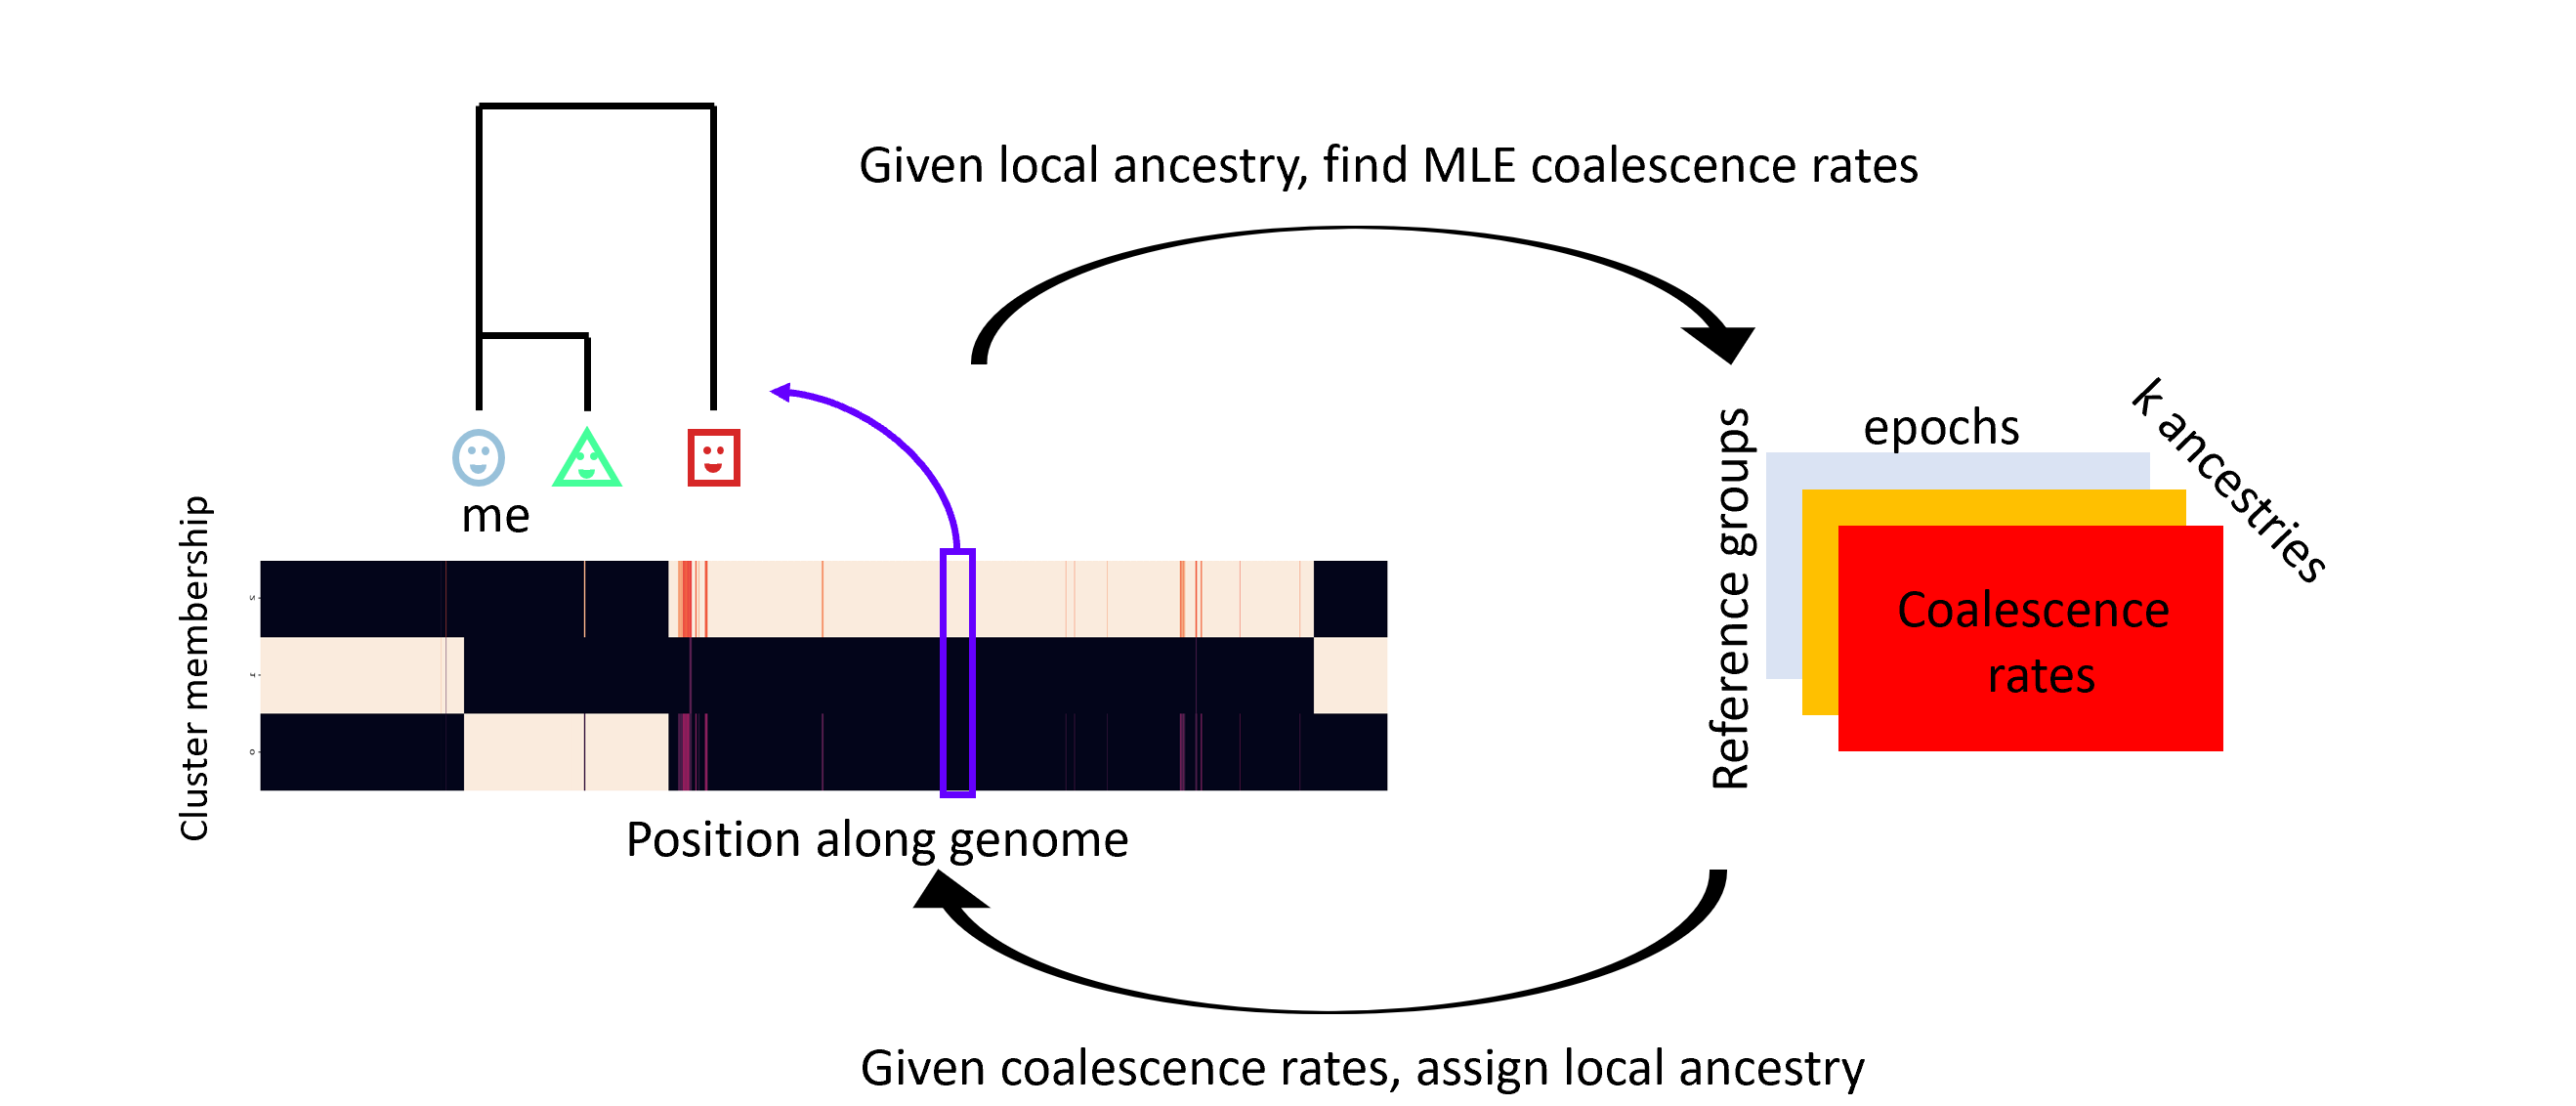
\includegraphics[scale=0.5]{figures/ghostbuster_method.PNG}
    \caption{\textbf{Overview of the GhostBuster algorithm.} The EM algorithm computes a local maximum likelihood estimate (MLE) for the mixture model, clustering regions of the genome based on variations in coalescence histories for a given target individual. The E-step calculates the expected log-likelihood of the data (in our case, the coalescence times with reference individuals) conditioned on the local tree topology and previous estimates of the model parameters (proportions, admixture time, and coalescence rates). We then use a HMM to infer the local ancestry of the target individual. The emissions for the HMM are modeled using the likelihood of the coalescence times, while the transitions are modeled using a Poisson process depending on recombination rates. In the M-step, we maximize the expected log-likelihood calculated in the E-step to obtain a new estimate of the model parameters. Under the EM algorithm, this process guarantees non-decreasing likelihood updates, leading to convergence at a local optimum \cite{dempster1977maximum}. The likelihood we derive conditions on the tree topology by carefully counting lineage contribution based on its descendants, which results in higher statistical power to detect admixture events in our analysis, as we do not assume reference individuals are independent or rely on any composite likelihood assumptions. A more detailed proof of the likelihood and the EM algorithm updates can be found in Section \ref{sec:ch2-gb-theory}.}
    \label{fig:gb_overview}
\end{figure}


\subsection{PCA visualization to visualize ancestral components}

To visualize the clustering performed by GhostBuster, we perform Principal Component Analysis (PCA) on the coalescence count and opportunity matrices obtained from the genealogies. The coalescence count matrix is an $N_{\text{ref}} \times N_{\text{sites}}$ matrix, where the $(g, l)^{\text{th}}$ entry represents the total contribution of reference group $g$ to the coalescence events at genomic position $l$. We aggregate the contributions from all coalescence events at genomic position $l$ between the target and reference individuals, considering only those events occurring within predefined start and end time epochs, which align with the start and end epochs used in the GhostBuster analysis. These epochs control the time periods in which we expect to observe differences in coalescence patterns. We construct a similar matrix for the opportunity, also an $N_{\text{ref}} \times N_{\text{sites}}$ matrix, where each entry $g,l$ records the total opportunity for reference group $g$ at position $l$. The same time epochs are used as in the coalescence count matrix to ensure consistency.

The coalescence count and opportunity matrices are then stacked to form a $2N_{\text{ref}} \times N_{\text{sites}}$ matrix, which is mean-centered and standardized. We perform eigen-decomposition on this matrix to obtain the leading principal components. These principal components provide a visual interpretation of the clustering performed by GhostBuster, helping to better understand the patterns in coalescence across the genome.

\subsection{Coancestry curves to date admixture event}
\label{sec:ch2-gb-coancestry}

Given the local ancestry inferred using GhostBuster, we use coancestry curves to accurately estimate the date of the admixture event.
%
As outlined in Section \ref{sec:ch1-gb-survey}, the joint probability of observing ancestry at a genetic distance \( g \) under a single-pulse admixture model is given by:
\begin{align}
    p_{AA}(g) &= \alpha^2 + \alpha (1 - \alpha) \exp(-g \lambda) \nonumber \\
    p_{AB}(g) &= \alpha (1 - \alpha) - \alpha (1 - \alpha) \exp(-g \lambda) \nonumber \\
    p_{BB}(g) &= (1-\alpha)^2 + \alpha (1 - \alpha) \exp(-g \lambda)
\end{align}
where $\alpha$ is the genome-wide proportion of ancestry `A', $1-\alpha$ of ancestry `B' and $\lambda$ is the admixture time in generations. We also consider admixture models with two-dates corresponding to two-pulses of gene flow. The joint probability of observing ancestry at a genetic distance \( g \) under a double admixture model is given by:

\begin{small}
\begin{align}
p_{AA}(g) &= \alpha_1^2 (1 - \alpha_3)^2 + \alpha_1^2 \alpha_3 (1 - \alpha_3) \exp(-g \lambda_2) 
+ \alpha_1 \alpha_2 (1 - \alpha_3) \exp(-g \lambda_1) \nonumber \\
p_{BB}(g) &= \alpha_2^2 (1 - \alpha_3)^2 + \alpha_2^2 \alpha_3 (1 - \alpha_3) \exp(-g \lambda_2) 
+ \alpha_1 \alpha_2 (1 - \alpha_3) \exp(-g \lambda_1) \nonumber \\
p_{AB}(g) &= p_{BA}(g) = \alpha_1 \alpha_2 (1 - \alpha_3)^2 
+ \alpha_1 \alpha_2 \alpha_3 (1 - \alpha_3) \exp(-g \lambda_2) 
- \alpha_1 \alpha_2 (1 - \alpha_3) \exp(-g \lambda_1) \nonumber \\
p_{CA}(g) &= p_{AC}(g) = \alpha_3 (1 - \alpha_3) \alpha_1 
- \alpha_3 (1 - \alpha_3) \alpha_1 \exp(-g \lambda_2) \nonumber \\
p_{CB}(g) &= p_{BC}(g) = \alpha_3 (1 - \alpha_3) \alpha_2 
- \alpha_3 (1 - \alpha_3) \alpha_2 \exp(-g \lambda_2) \nonumber \\
p_{CC}(g) &= \alpha_3^2 + \alpha_3 (1 - \alpha_3) \exp(-g \lambda_2)
\end{align}
\end{small}
where, $\alpha_1(1-\alpha_3)$ is the genome-wide proportion of ancestry `A', $\alpha_2(1-\alpha_3)$ of ancestry `B', $\alpha_3$ of ancestry `C' and $\lambda_1$, $\lambda_2$ are the corresponding admixture times. Finally, we consider admixture models corresponding to constant migration rate continuous admixture. In this case the joint probability of observing ancestry at a genetic distance \( g \) is given by:
\begin{align}
p_{AA}(g) &= \alpha^2 + \alpha (1 - \alpha) \sum_{j = \lambda_e}^{\lambda_s} w_j \exp(-g j) \nonumber \\
p_{AB}(g) &= \alpha (1 - \alpha) - \alpha (1 - \alpha) \sum_{j = \lambda_e}^{\lambda_s} w_j \exp(-g j) \nonumber \\
p_{BB}(g) &= (1-\alpha)^2 + \alpha (1 - \alpha) \sum_{j = \lambda_e}^{\lambda_s} w_j \exp(-g j)
\end{align}
where, $w_j = \frac{\mu (1 - \mu)^{\lambda_s - j}}{1 - (1 - \mu)^{\lambda_s - \lambda_e + 1}}$; $\lambda_s$ and $\lambda_e$ are the start and end time of the admixture, $\mu$ is the constant migration rate. Detailed derivation of the analytical coancestry curves can be found in the supplementary information of \cite{hellenthal2014genetic}.

We fit the exponential distribution to all possible ancestry combinations and jointly maximize the log-likelihood. 
%
In the case of three-way or more complex admixture, we fit coancestry curves for each pair of ancestries separately, estimating the dates for each event independently.
%
We use 20 block-jackknife across chromosomes to estimate standard errors when dating the admixture event.
% 
Additionally, we use diploid ancestry calls (summing the posteriors of two haplotypes) to prevent phasing errors from biasing the admixture dating.

Genetic drift can cause the fixation or loss of certain alleles, introducing a downward bias in the dating estimates derived from coancestry curves. This effect is particularly pronounced in small populations or when considering ancient events, where the influence of drift is much greater. To mitigate this bias, we normalize the coancestry curves by the coancestry curves generated from randomly sampling haplotype pairs from different individuals, also known as pseudo-individuals. As previously done in Globetrotter \cite{hellenthal2014genetic}, this approach corrects for the impact of genetic drift and provides an unbiased admixture date.

Another source of error in admixture dating can arise from inaccuracies in recombination maps. This is particularly relevant for dating ancient events, where errors on the scale of tens of kilo-bases in the recombination map can downward-bias the inferred date \cite{sankararaman2012date}. In our case, this issue does not affect the simulated examples, as we assume a perfect recombination map, but might have some impact on real data, especially the old admixture dates. However, due to the lack of suitable error estimates for the recombination map of the population being analyzed, we highlight this as a cautionary note for the interpretation of results from real data. %To still account for potential errors, we apply a correction based on the factor introduced by \cite{sankararaman2012date}, which compares fine-scale recombination maps derived from pedigrees with those based on European LD patterns. Although this correction is approximate, it provides a useful adjustment.

Finally, the effects of selection and the evolution of recombination maps can influence admixture dates; however, we assume these factors have a minimal impact on our real-data examples.

\subsection{Joint analysis of multiple targets}
Sometimes the reference populations can be themselves admixed.
%
GhostBuster allows estimating the coalescence rates of the target lineage with reference populations conditioned on the local ancestry of the reference populations.
%
It does so by counting coalescence events and opportunity separately for different ancestries in the admixed reference populations.

It is also possible that the reference populations share the same admixture event as the target individual. To account for this, we employ a two-step procedure to fit the admixture event. First, we fit a mixture model assuming unadmixed reference populations, assigning ancestry to all admixed reference populations. Next, we threshold the inferred local ancestry probabilities for the reference populations and refit the mixture model conditioned on this local ancestry. This method allows for an approximate joint fitting of multiple target individuals.

\subsection{Tree Filtering}

We only consider trees every $10$kb apart, ensuring the tree intervals overlap with the local ancestry grid at least once.
%
% Additionally, for fitting the mixture model, we only retain trees which correspond to bottom 50\% of the recombination rates, where the recombination rate is calculated 500kb around the tree.
% %
% These trees usually have more mutations to support the tree topology and are therefore more accurate.
%
We filter out trees in regions corresponding to centromeres, telomeres, and the HLA gene, along with a $500$kb buffer around these areas. The positions of centromeres, telomeres, and the HLA region in the appropriate genome build were obtained from the \href{https://genome.ucsc.edu/goldenPath/help/ftp.html}{here}.
%
% Once the per-component coalescence rates and proportions are inferred we utilize them to infer the local ancestry of the whole genome including regions with high recombination rates.

\subsection{Choosing the number of components}
\label{sec:ch2-gb-selecting-clusters}

A critical aspect of decomposing local ancestry is selecting the optimal number of components for our method. To ensure we determine the appropriate number, we conduct several tests to evaluate and optimize this choice.

First, we assess the model’s log-likelihood on an independent, held-out chromosome. This allows us to distinguish admixture events that replicate consistently across chromosomes from biases that are chromosome-specific and do not generalize well. The evaluation proceeds as follows: we estimate the parameters—such as coalescence rates and proportions—using our EM algorithm on data from all chromosomes except the held-out one (by default we use chromosomes 2-5). We then use the fitted parameters to calculate the log-likelihood on the held-out chromosome (by default we use chromosome 1), without relying on the HMM. The optimal number of components is identified by selecting the point where the total log-likelihood across held-out chromosomes is maximized.

Second, we analyze the posterior probabilities of local ancestry by plotting a histogram of the target ancestry and calculating the expected coefficient of determination (expected $R^2$), as defined in \cite{price2009sensitive,salter2019fine}. Expected $R^2$ estimates the correlation between true and inferred local ancestry, assuming the true local ancestry follows a Bernoulli distribution with the same mean as the inferred one. Both the histogram and expected $R^2$ help assess the confidence of the cluster assignments, where values greater than 0.7 generally indicate reliable local ancestry inference. 

The expected $R^2$ between true (denoted as $X$) and predicted local ancestry estimates (denoted as $Y$) can be calculated as follows:

\begin{align}
    \mathbb{E}(R^2_{XY}) &= \mathbb{E} \left( \frac{\text{cov}(X, Y)^2}{\text{Var}(Y) \text{Var}(X)} \right) \\
              &\approx \frac{\mathbb{E}(\text{cov}(X, Y))^2}{\text{Var}(Y) \mathbb{E}(\text{Var}(X))}
\label{eq:expected_r}
\end{align}

Assuming the true local ancestry to follow Bernoulli distribution with same empirical mean as predicted local ancestry, $P(X_g = 1) = Y_g$. Where, $g$ indexes the local ancestry position (total = $G$) along the genome. We can evaluate the terms in equation \ref{eq:expected_r} as follows:
\begin{align}
\text{var}(Y) &= \frac{\sum_g Y_{g}^2}{G} - \left( \frac{\sum_g Y_{g}}{G} \right)^2 \nonumber \\ 
\mathbb{E}[\text{cov}(X, Y)] &= \mathbb{E} \left[ \frac{\sum_g X_{g} Y_{g}}{G} - \frac{\sum_g Y_{g}}{G} \frac{\sum_g X_{g}}{G} \right] \nonumber  \\
&= \frac{\sum_g Y_{g} \mathbb{E}[X_{g}]}{G} - \frac{\sum_g Y_{g}}{G} \frac{\sum_g \mathbb{E}[X_{g}]}{G} \nonumber \\
&= \frac{\sum_g Y_{g}^2}{G} - \left( \frac{\sum_g Y_{g}}{G} \right)^2 \nonumber \\
\mathbb{E}[\text{var}(Y)] &= \mathbb{E} \left[ \frac{\sum_g X_{g}^2}{G} - \left( \frac{\sum_g X_{g}}{G} \right)^2 \right] \nonumber  \\
&= \frac{\sum_g \mathbb{E}[X_{g}]^2}{G} + \text{var}(X_{g}) - \left( \frac{\sum_g \mathbb{E}[X_{g}]}{G} \right)^2 \nonumber  \\
&= \frac{\sum_g Y_{g}^2 + Y_{g} (1 - Y_{g})}{G} - \left( \frac{\sum_g Y_{g}}{G} \right)^2 \nonumber  \\
&= \frac{\sum_g Y_{g}}{G} - \left( \frac{\sum_g Y_{g}}{G} \right)^2
\end{align}

Finally the $\mathbb{E}(R^2_{XY})$ is given as:
\begin{align}
    \mathbb{E}(R^2_{XY}) &\simeq \frac{\left( \sum_g Y_{g}^2 - \left( \sum_g Y_{g} \right)^2/G \right)}{\sum_g Y_{g} - \left( \sum_g Y_{g} \right)^2/G}.
\label{eq:expected_r_final}
\end{align}
We use a diploid version of the equation \ref{eq:expected_r_final} which sums the local ancestry for both haploids; more details and derivation for the diploid version can be found in \cite{salter2019fine}. 

Finally, we use the inferred local ancestry to perform coancestry curve-based dating of the admixture event. Unlike admixture tracts, which correspond to long ancestry segments, general biases tend to result in much older estimated dates. Admixture dates exceeding 2,500 generations are challenging to distinguish from genuine events and are typically regarded with caution, as they may reflect biases in genealogical inference rather than true admixture.

While this approach performs well in simulations, real data introduces additional complexities. The full admixture history of a sample is often intricate, and source populations themselves may be the result of earlier admixture. Thus, in practice, we select the number of components based on how well the components can be interpreted in the context of real data. In most cases, this results in choosing two components. Ultimately, the choice of the number of components can be data-driven, guided by the held-out log-likelihood, expected $R^2$, and coancestry dating, or informed by prior knowledge of the admixture event.

\subsection{Calculation of node persistence}
\label{sec:ch2-gb-node-persistence}
The majority of nodes in adjacent trees are shared. Accurate calculation of node persistence is critical in our likelihood estimation, as it prevents the over-counting of identical or similar coalescence events. In true genealogies, nodes can be distinguished by their coalescence times. These coalescence times remain consistent across adjacent trees unless a recombination event affects the corresponding node.

However, in inferred genealogies, the coalescence times are not precisely identical, even in the absence of recombination, as each tree is dated independently based on its structure. To identify equivalent nodes in inferred genealogies, we examine the descendant composition of these nodes. Specifically, we store a vector of length equal to the number of samples, representing the descendant composition of the lineage coalescing with the target lineage. In this vector, the $m$th entry is set to 1 if haplotype $m$ descends from the coalescence event, and 0 otherwise. Similar to defining equivalent branches in Relate \cite{speidel2019method}, we define two nodes as equivalent if the correlation coefficient between their descendant composition vectors exceeds a predefined threshold (default = 0.5). To ensure that each node is matched with at most one other node, we rank pairs of candidate nodes in descending order of their correlation coefficient. Nodes are then associated based on their position in this sorted list, with any pair involving a node already associated with another node being removed.

In true genealogies, where we have access to actual node persistence, we observed that the approximate node persistence reasonably aligns with the true values (see Figure \ref{fig:gb_node_persistence} for comparison).

\begin{figure}
    \centering
    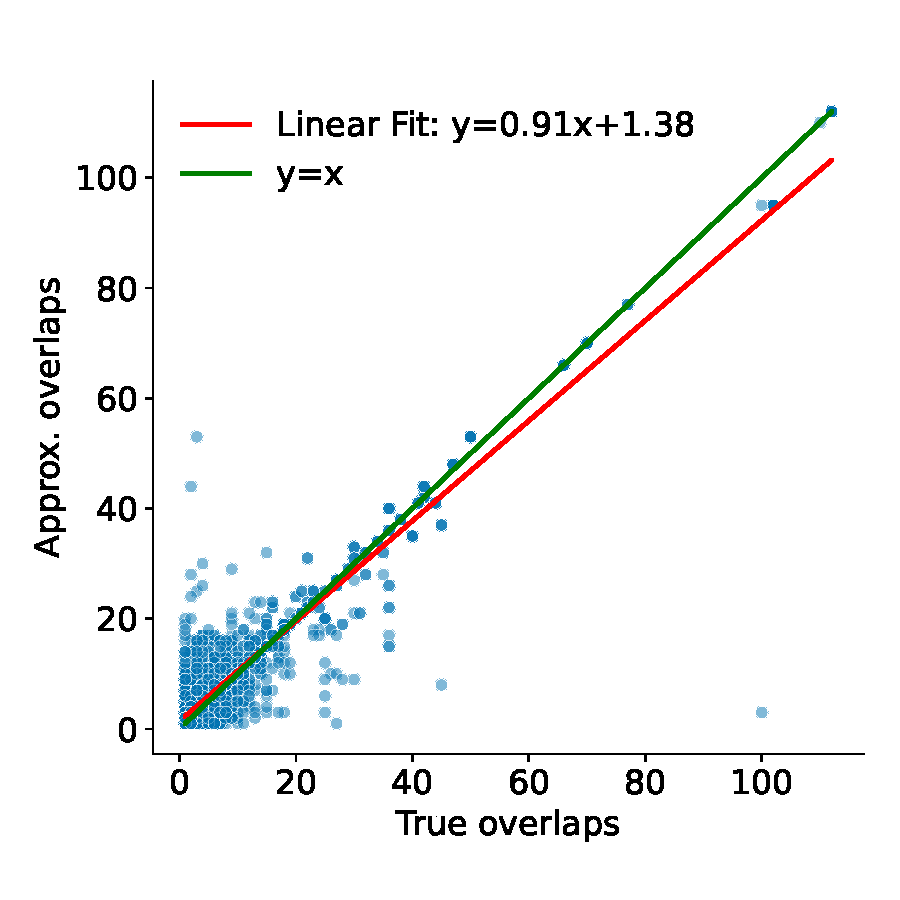
\includegraphics[width=0.5\linewidth]{figures/node_persistence_comparisons_0.5.pdf}
    \caption{\textbf{Comparison of Approximate and True Node Persistence in Simulated Trees.} True node persistence is determined by identifying the exact coalescence times across neighboring trees, while approximate node persistence is estimated based on the correlation of descendant sets between adjacent trees. In this case, the correlation cutoff for approximate node persistence is set to 0.5, with the number of overlaps indicating the number of $10$kb intervals for which the node persists.}
    \label{fig:gb_node_persistence}
\end{figure}

\subsection{Handling uncertain coalescence events}
\label{sec:ch2-gb-uncertain-coal}
Since the mutation and recombination rates in humans are approximately similar, multiple tree structures often exist to explain the genetic variation at a given site, making genealogy inference uncertain and potentially inaccurate. To address this uncertainty, we scale the likelihood of our mixture model based on the confidence in coalescence events, which is evaluated by the presence of mutations above the node.

Specifically, we trace the coalescence events along the target lineage backward in time, identifying subsets of nodes (or coalescence events) that are jointly supported by at least one mutation (see Figure \ref{fig:gb_uncertainty_nodes}). For each subset, we calculate the expected number of coalescence events (or nodes) that are supported by mutations. To clarify, this is equivalent to asking: what is the expected number of coalescence involving the target lineage if the coalescence events between the lineages were shuffled randomly? We assume that clades coalescing with the target are resolved—that is, they have mutations supporting their tree structure. We further assume that unresolved coalescence events occur around the same time, simplifying their contribution to the likelihood. The expected number of coalescence events, conditioned on the presence of $C$ unresolved events, can be computed as the sum of the probability of coalescing with the target for the $C$ independent coalescence events.
\begin{align}
    \mathcal{E}[C] &= \sum_{i=1}^{C} \frac{i}{\binom{i+1}{2}} \\
    &= \sum_{i=1}^{C} \frac{2}{i+1}
\end{align}

We scale the likelihood for each node by the expected number of coalescence events divided by the observed number of coalescence events, that is $\frac{\mathcal{E}[C]}{C}$. For cases where there are 1, 2, or 3 unresolved nodes, the corresponding expected number of coalescence events equals $1$, $\frac{5}{3}$, and $\frac{13}{6}$, leading to effectively scaling the likelihood by $1$, $\frac{5}{6}$, and $\frac{13}{18}$, respectively.

\begin{figure}
    \centering
    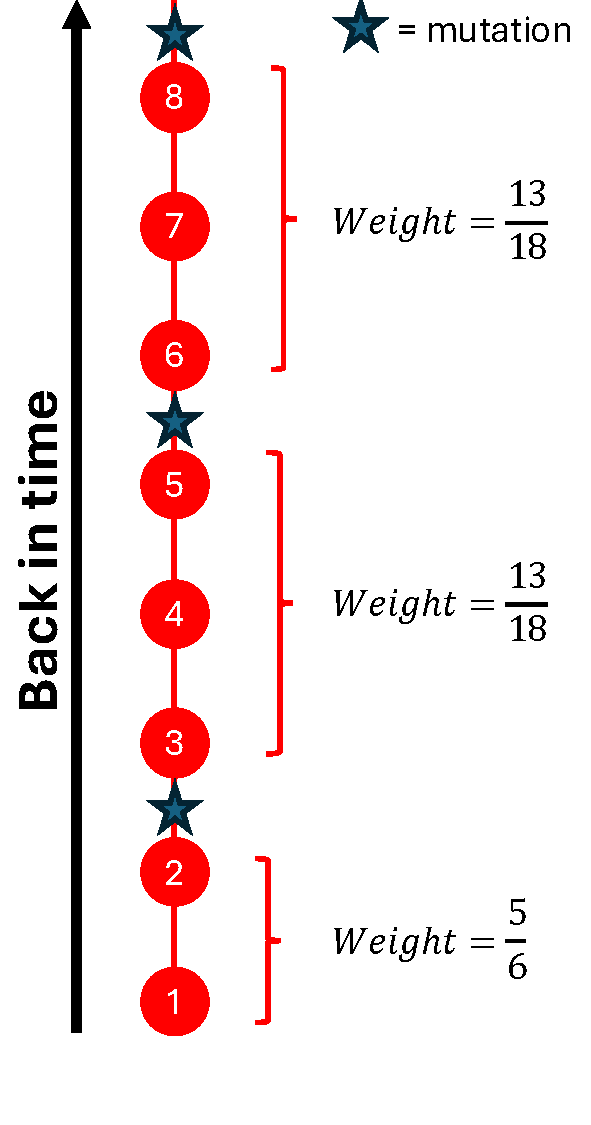
\includegraphics[width=0.5\linewidth]{figures/thesis_gb_uncertainty_nodes.pdf}
    \caption{\textbf{Handling uncertainty in coalescence events.} We calculate the expected number of coalescence events for subsets of nodes jointly supported by a mutation. In this example, there are three such subsets on the target lineage, with weights for each coalescence event calculated based on the number of nodes in the subset.}
    \label{fig:gb_uncertainty_nodes}
\end{figure}


\subsection{Initialization}
To approximate a solution near the global maximum, we perform a random search over 20 randomly initialized values for coalescence rates, proportions, and admixture times. The coalescence rates are sampled from a log-uniform distribution within the range [$5 \times 10^{-2}$, $1 \times 10^{-7}$]. The proportions are drawn from a uniform distribution between 0.01 and 0.99, while the admixture times are sampled from a log-uniform distribution spanning 20 to 2000 generations. For each random initialization, the EM algorithm is run for 10 iterations. The initialization that achieves the highest log-likelihood after these iterations is selected as the optimal starting point for further model fitting.

\section{Data and quality control}
\label{sec:ch2-gb-data}
\subsection{Modern human datasets}

We work with multiple publicly available modern human datasets throughout our analysis. The datasets we analyze include the Human Genome Diversity Project (HGDP) \cite{cann2002human, bergstrom2020insights}, Simons Genome Diversity Project (SGDP) \cite{mallick2016simons}, and $1{,}000$ Genomes Project ($1{,}000$ GP) \cite{sudmant2015integrated, 10002015global}.
%
The whole-genome sequenced version of HGDP \cite{bergstrom2020insights} comprises 929 individuals and 51 diverse population groups sampled across the globe, with an average coverage of $34 \times$ (range: $23$-$75 \times$).
%
The $1{,}000$ GP dataset comprises 2,504 individuals from 26 populations across the globe, with an average coverage of $32 \times$ (range: $26$-$66 \times$).
%
The SGDP dataset comprises 278 individuals from 142 diverse populations across the globe, with an average coverage of $43 \times$ (range: $34$-$83 \times$).

In particular, we use the unified version of HGDP and $1{,}000$ GP \cite{koenig2024harmonized}, where the genomes from the two projects were jointly called.
%
We obtained the phased version of the dataset from \href{gs://gcp-public-data‐‐gnomad/resources/hgdp_1kg/phased_haplotypes_v2/}{here}. This dataset was called with the hg38 genome build.
%
The phased data had already undergone variant QC to filter variants with (1) HWE $\geq 1 \times 10^{-30}$, (2) F\_MISSING $\leq 0.1$, or (3) ExcHet $\geq 0.5$ and ExcHet $\leq 1.5$.
%
We additionally excluded multi-allelic SNPs and Indels from the dataset.
%
We also performed sample QC, retaining only a subset of African samples from the $1{,}000$ GP (20 individuals per 6 African subgroups: `ACB', `ASW', `ESN', `LWK', `GWD', `MSL') and removing close relatives up to the 2nd degree.
%
To remove relatives, we used the list of unrelated samples in HGDP + $1{,}000$ GP inferred in the Allen Ancient DNA Resource \cite{mallick2024allen} and retained only individuals falling within this set.
%
Finally, we retained 45.6 million variants and 1,026 samples across 58 population groups in this dataset.

The Simons Genome Diversity Project (SGDP) was called in the hg37 genome build and was therefore not merged with the HGDP + $1{,}000$ GP dataset.
%
We treated it separately as an independent validation dataset.
%
The phased data for SGDP was obtained from \href{https://sharehost.hms.harvard.edu/genetics/reich_lab/sgdp/phased_data.knownbugs.not_recommended.please_use_newer_dataset_instead/}{here}.
%
Apart from the filtering done in \cite{mallick2016simons}, we additionally excluded multi-allelic SNPs and Indels from our analysis.
%
We retained 28.3 million variants and 278 samples across 130 population groups in this dataset.

\subsection{High quality ancient DNA resources}

The assembly and quality control of the ancient DNA dataset were performed by Dr. Leo Speidel, who is one of the co-authors on the paper.
%
Apart from the modern samples, we also consider 49 ancient DNA and 4 archaic DNA samples. These samples were all high coverage, with an average coverage of $17.3\times$ (range: $10.3$-$65.1 \times$). The ancient and archaic DNA samples used in the analysis are tabulated in \ref{tab:gb_ancient_samples}.

The ancient DNA BAM files were processed using \texttt{bcftools mpileup} to generate variant calls, selecting only reads with a mapping quality of 20 or higher, a base quality of 20 or higher, and a minimum depth of coverage of 5.
%
The variant calls from the ancient DNA samples were then merged with the $1{,}000$ GP (downloaded from \href{https://ftp.1000genomes.ebi.ac.uk/vol1/ftp/release/20130502/}{here}) and phased using \texttt{shapeit4}. The phasing process involved first phasing variants observed in $1{,}000$ GP and then using the phasing as a scaffold to phase variants not observed in $1{,}000$ GP within the ancient dataset. We additionally randomly phased singletons in the ancient dataset.
%
Subsequently, the ancient DNA dataset was lifted over to the hg38 reference genome using \texttt{picard LiftoverVcf} and merged with the unified version of HGDP + $1{,}000$ GP using the \texttt{bcftools merge -0} option. This merging resulted in less than $0.001$\% missingness. After merging, we filtered out multi-allelic variants, duplicate variants, and indels. As a final sanity check, we compared allele frequencies between the HGDP + $1{,}000$ GP dataset and the ancient DNA dataset, finding a high correlation between the allele frequencies with minimal missingness (see Figure \ref{fig:gb-sanity-check}).

\subsection{Building genome-wide genealogies for moderns and ancients}

We use Relate \cite{speidel2019method} to construct genealogies from phased data for both modern and ancient samples. For genealogies involving only modern samples, we apply a genomic mask provided with $1{,}000$ Genomes Project (lifting it for hg38 datasets), retaining only regions marked as "passing" to exclude variants with high uncertainty. Additionally, we mask sites where the human ancestral allele FASTA file (accessible \href{ftp://ftp.ensembl.org/pub/release-74/fasta/ancestral_alleles/homo_sapiens_ancestor_GRCh37_e71.tar.bz2}{here}) shows missing data, as well as sites corresponding to multi-allelic SNPs or indels. For genealogies that include archaic samples, we further refine this mask by considering only sites that pass in all Neanderthal and Denisovan masks (accessible \href{http://ftp.eva.mpg.de/neandertal/}{here}). Additionally, for genealogies with ancient samples, we filter out sites where ancient samples exhibit more than 10\% missingness. The masks corresponding to ancient and archaic samples are lifted over to the hg38 reference genome to ensure consistency.

To identify the most likely ancestral allele for each SNP, we use an estimate of the human ancestral genome. We utilize the HapMap3 inferred recombination rate maps for builds hg37 and hg38, which can be downloaded \href{https://github.com/odelaneau/shapeit5/tree/main/resources/maps/}{here}. The mutation rate is set to $1.25 \times 10^{-8}$ for building genealogies of modern samples, while for genealogies involving ancient or archaic samples, the mutation rate is adjusted to $1.2 \times 10^{-9}$, and all CpGs are excluded from genealogy inference. To ensure consistency in the genealogies, we enforce the construction of topologies every $10$kb using the \texttt{--fb} option. When working with ancient samples, we provide the estimated ages of the samples to improve the accuracy of the genealogies. The population size of the sample is estimated by iteratively fitting the population sizes and branch lengths for chromosome 1, over five iterations. The converged population size is then used as a prior for dating branch lengths on the remaining chromosomes. Finally, the resulting trees are converted to tskit format, retaining only the trees to be used for model fitting in GhostBuster.

Due to differences in variant filtering and genome build, we construct multiple genealogies for distinct sets of samples. The genealogies include:  
\begin{enumerate}
    \item \textbf{HGDP + $1{,}000$GP}: Comprises all modern samples from HGDP and a subet of African samples from $1{,}000$ Genomes Project.  
    \item \textbf{HGDP + $1{,}000$GP + aDNA}: Includes HGDP + $1{,}000$GP samples along with 49 high-coverage ancient DNA samples.  
    \item \textbf{HGDP + $1{,}000$GP + aDNA + archaic}: Extends the HGDP + $1{,}000$GP + aDNA set by adding 4 archaic samples.  
    \item \textbf{SGDP}: Contains all modern samples from SGDP.  
\end{enumerate}  
We verified our inferred genealogy for all sample sets by evaluating the inferred inverse coalescence rates between populations (see Figures \ref{fig:gb_pairwise_coal_hgdp_1gp}, \ref{fig:gb_pairwise_coal_hgdp_1gp_adna}, \ref{fig:gb_pairwise_coal_hgdp_1gp_archaic}, \ref{fig:gb_pairwise_coal_sgdp}, \ref{fig:gb_pairwise_coal_europe_3way}). For real data analysis of population structure in Africa (Chapter \ref{ch:3-gb-result}), we primarily focus on using samples from HGDP and 1,000GP, while incorporating SGDP samples to augment the analyses where feasible.

\section{Accurate local ancestry inference in simulations}
\label{sec:ch2-gb-sim}
\subsection{Simulation design}
\label{sec:ch2-gb-sim-design}

To assess the power and robustness of detecting ghost populations, we simulate two distinct admixture scenarios: a four-way recent admixture and Denisovan admixture into Papuans. For both simulations, we used a constant mutation rate of $1.25 \times 10^{-8}$ and the HapMap3 recombination rate map, excluding regions with zero recombination rate, centromeres, telomeres and the HLA region on chromosome 6. We simulate demography using \texttt{ msprime} \cite{kelleher2016efficient}.

\begin{enumerate}
    \item \textbf{Four-way recent admixture:} In this scenario, we assume four reference populations (A, B, C, and D), each contributing 25\% to form the focal individual 5,000 years ago. Populations A and B split $50{,}000$ years ago, as did populations C and D, with all populations merging back together $100{,}000$ years ago (Figure \ref{fig:sim1}a). We assume a constant population size of $20{,}000$ for all populations after their split and $10{,}000$ for the super-populations prior to $50{,}000$ years ago. To assess the case without a ghost population, we sample 10 diploid individuals from each population and five focal (admixed) individuals. For the ghost population scenario, we sample 10 individuals each from populations A, B, and C, with none from population D.
    
    \item \textbf{Denisovan Introgression into Papuans:} This scenario uses the simulation model and script provided by \cite{skov2018detecting} to simulate Denisovan introgression into Papuans. We assume three reference populations (Papuans, Africans, and Denisovans), where Papuans and Africans split $72{,}036$ years ago, and Denisovans split from modern humans $656{,}908$ years ago (Figure \ref{fig:sim1}b). Denisovans admixed with Papuans around $43{,}935$ years ago with a 5\% admixture proportion. The population sizes are $3,899$ for modern Papuans, $27{,}122$ for Africans, and $4{,}947$ for Denisovans before they went extinct. We also simulate the Out-of-Africa bottleneck, where the Papuan population size drops to $136$. A graphic overview of this simulation is shown in Figure \ref{fig:sim1}b. We fit five Papuan individuals, using 25 Papuans and 25 Africans as the reference panel. Additionally, we assess the power and compare local ancestry estimates with and without an ancient Denisovan sample dated to 67,570 years ago.
\end{enumerate}

\begin{figure}
    \centering
    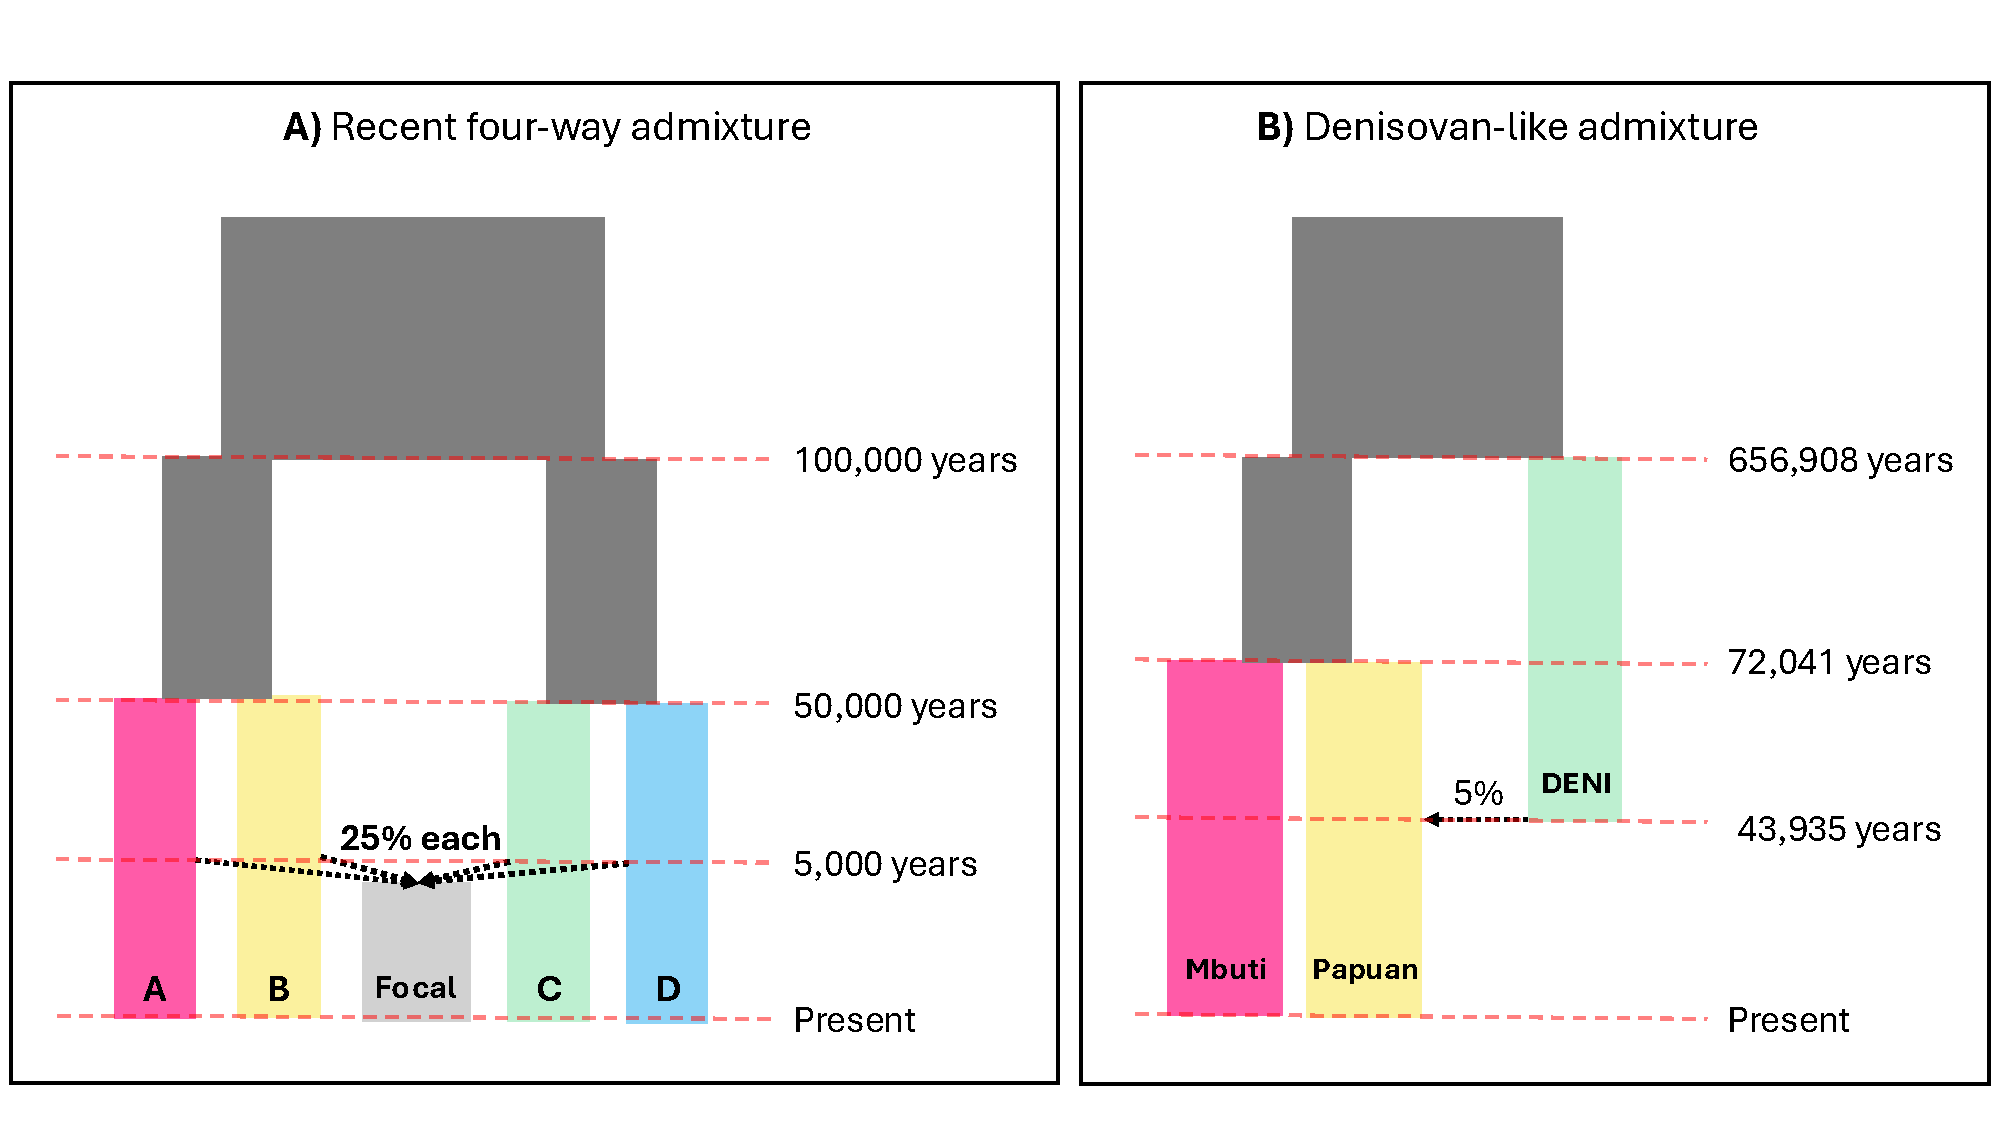
\includegraphics[width=\textwidth]{figures/thesis_gb_sim_design.pdf}
    \caption{\textbf{Simulation design for performance evaluation.} A. Four-way recent admixture simulation, B. Simulated Neanderthal introgression into Han Chinese. The simulation parameters including the population size, mutation rate and recombination map are described in section \ref{sec:ch2-gb-sim-design}.}
    \label{fig:sim1}
\end{figure}

\subsection{Four-way recent admixture}

%% para 1
% How many individuals we simulate, whats the target, whats the reference? 
% number of chromosomes? 
% We expect a 4-way admixture (see simulation design section)
% We run the method on both true trees and relate trees inferred using the variation data

We validated GhostBuster's ability to detect admixture events through a simple simulation, where we modeled a recent 4-way admixture event occurring 5,000 years ago, involving groups that had been separated for at least 50,000 years (see Figure \ref{fig:sim1}a). The focal individual in our simulation resulted from an equal contribution of 25\% ancestry from four distinct reference populations, labeled A, B, C, and D. We sampled up to 10 individuals from each reference population and used chromosomes 1 through 5. More details about the simulation setup can be found in Section \ref{sec:ch2-gb-sim-design}. Our objective was to decompose the focal individual's ancestry both with and without access to all reference populations, with the expectation of accurately identifying the four ancestral components. We applied our method primarily to trees inferred using genetic variation data via Relate, assuming a constant mutation rate of $1.25 \times 10^{-8}$, while results comparing with true trees simulated using msprime are also presented. Additionally, we only focused on coalescence events occurring from 0 to 50,000 years.

%% para 2
% We first tested the method with k=4 and presence of all reference groups
% We started with random init. and EM for 200 iterarions
% We found the four-components coal. rates represented four-populations (1 - a, 2 -b, ..)
% The coal. rates are more distinct and seperated for true trees than relate trees, representing the error in building genealogies 
% In order to compute the accuracy, we compared local ancestry with the true local ancestry R2 = 
% Calibration plots

We first tested the method with access to all four reference populations and applied our approach to decompose the focal individual's ancestry into four distinct components or clusters. Starting with a random initialization of coalescence rates and proportions, we fit our model over 200 EM iterations until the log-likelihood converged. The resulting inverse coalescence rates represent the four clusters that best differentiated the coalescence events for the focal individual (see Figure \ref{fig:gb_sim_four_nonghost}a). The inverse coalescence rate (ICR) for each component reflects its affinity toward one of the four reference populations—a lower ICR value indicates faster coalescence with that specific population. Our analysis revealed that the four clusters identified by GhostBuster contributed approximately 25\% to the focal individual's ancestry, with each cluster more closely related to one of the four reference populations. For example, component 1 was most similar to population D, component 2 to population A, component 3 to population C, and component 4 to population B. The clusters were clearly distinguishable using the top four principal components (PCs) of the coalescence count and opportunity matrices (see Figure \ref{fig:gb_sim_four_nonghost}b). Further evaluation based on the expected coefficient of determination and held-out log-likelihood indicated that four components provided the best fit to the data, with diminishing returns in held-out log-likelihood beyond four components (see Figure \ref{fig:gb_sim_four_nonghost}c). We also accurately dated the admixture event to $185.1$ generations, or $5{,}182.8$ years, using coancestry curves (see Figure \ref{fig:gb_sim_four_nonghost}d). Finally, we assessed the accuracy and calibration of our local ancestry inference by comparing it with the simulated ground truth, demonstrating strong correlation and low calibration error (see Figure \ref{fig:gb_sim_four_nonghost}e-g).

\begin{figure}[h!]
    \centering
    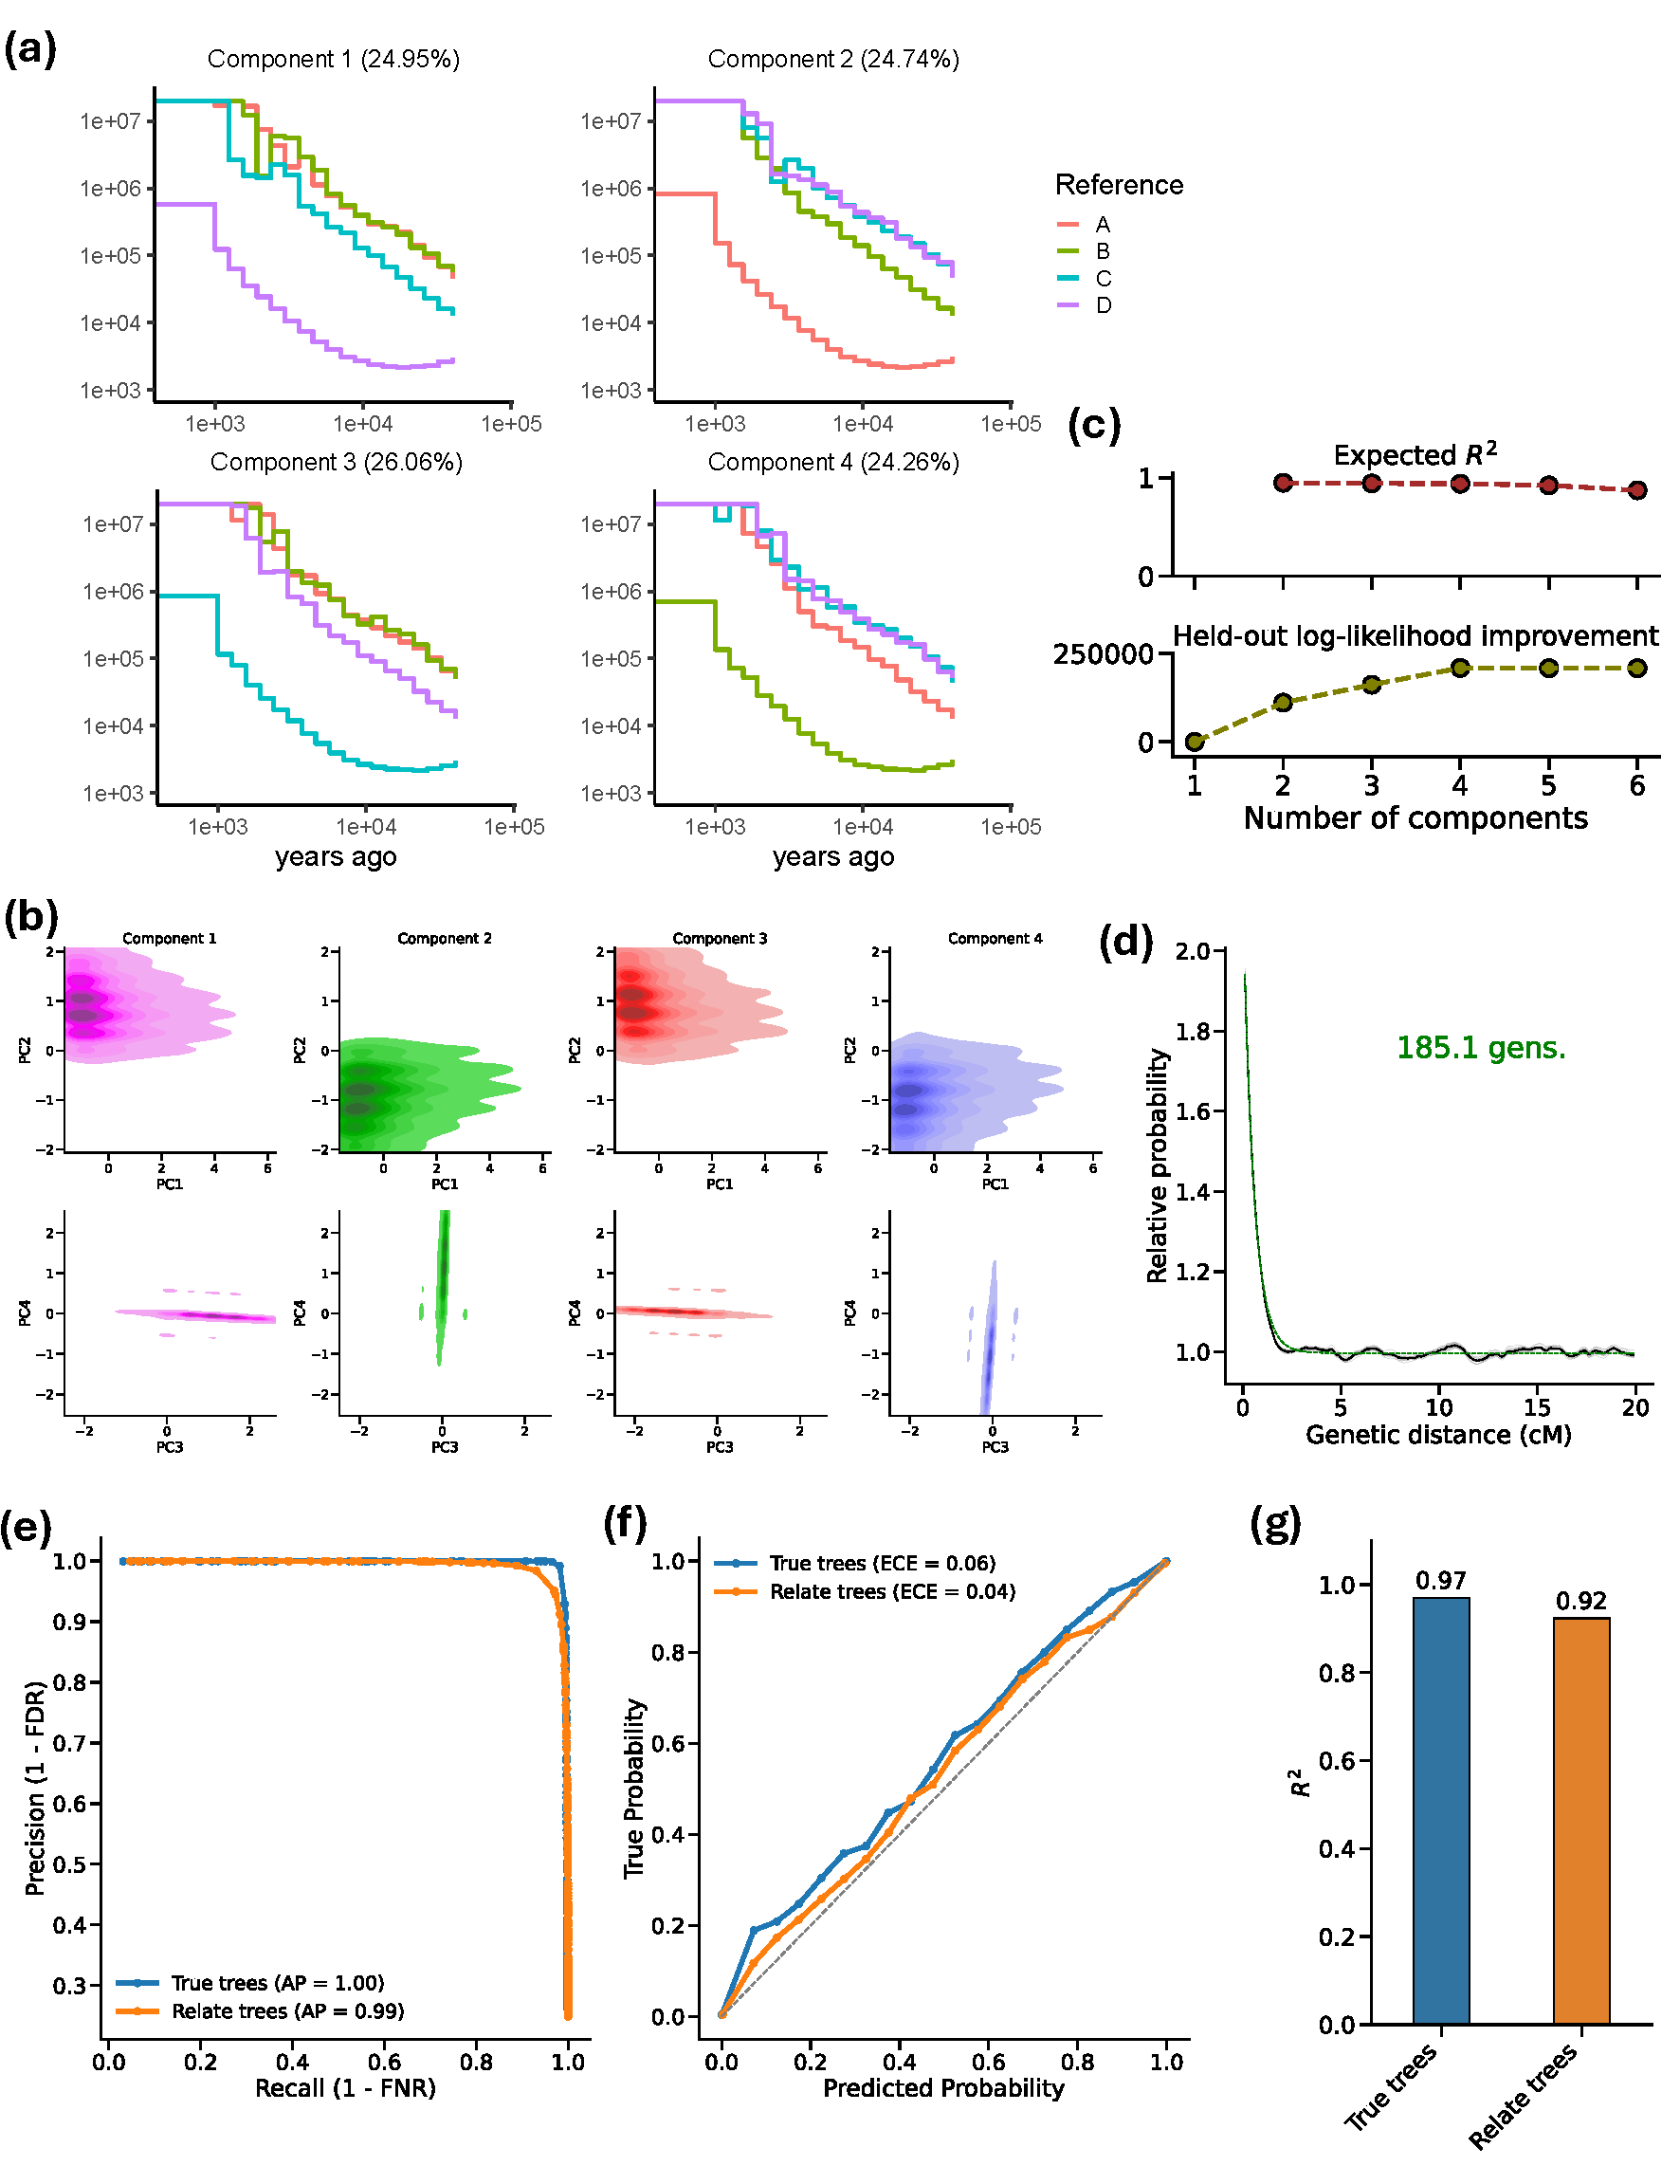
\includegraphics[width=\linewidth]{figures/gb_sims/gb_sim_4way_nonghost.pdf}
    \captionsetup{width=\textwidth+3cm}     \caption{
    \footnotesize
    \textbf{Decomposing focal individuals in the four-way admix simulation with presence of all source populations.} (a) Inferred inverse coalescence rates and proportions: each line represents inverse coalescence rate profiles with a reference population. (b) PCA visualization of the coalescence count and opportunity matrix derived from the genealogies plotted separately for each component. (c) Expected coefficient of determination and held-out log-likelihood improvement with varying number of components. (d) Coancestry curve for normalized joint probability of component 1 and the inferred admixture dates (in generations). (e) Precision-recall curves, (f) Calibration curves, and (g) Prediction $R^2$ for inferred local ancestry compared to the simulated ground truth, where inference was done using true trees or Relate trees. The PCA visualization in (b) is based on a KDE plot with a threshold of 0.05, and binary local ancestry estimates are obtained by thresholding the inferred posteriors at 0.5.
    }
    \label{fig:gb_sim_four_nonghost}
\end{figure}

%% para 3
% Next we removed population D from reference
% We did similar procedure with k = 4 
% four components, with the fourth component being distant from all 3 sampled reference populations
% local ancestry R2
% calibration plots

Next, we removed population D (without loss of generality) from the genealogies and attempted to decompose the focal individual. This scenario simulates the presence of a ghost population, as population D contributed to the focal individual's genetic makeup but is not included in the reference panel. We reran our method, fixing the number of components to four. The four components still contributed roughly 25\% to the total ancestry. The inverse coalescence rates (ICRs) for each component only existed for populations A, B, and C, as no individuals from population D were sampled. Component 2's ICR was closest to population B, component 3 was closest to population A, and component 4 was closest to population C (see Figure \ref{fig:gb_sim_four_ghost}a). However, component 1 was more distantly related to all three populations, indicating slower coalescence with each. This could be the ancestry relating to population D, which may have been tagged by its slower coalescence rates with populations A-C. Similar to the run with access to population D, we performed PCA visualization (Figure \ref{fig:gb_sim_four_ghost}b), evaluation of the number of clusters (Figure \ref{fig:gb_sim_four_ghost}c), coancestry curve dating (Figure \ref{fig:gb_sim_four_ghost}d), and accuracy and calibration of local ancestry inference (Figures \ref{fig:gb_sim_four_ghost}e-g). When comparing local ancestry with the simulated ground truth, we found a strong correlation, with an $R^2$ value of $0.88$, indicating that component 1 effectively captured the ancestry related to population D without requiring direct samples from that population.

\begin{figure}[h!]
    \centering
    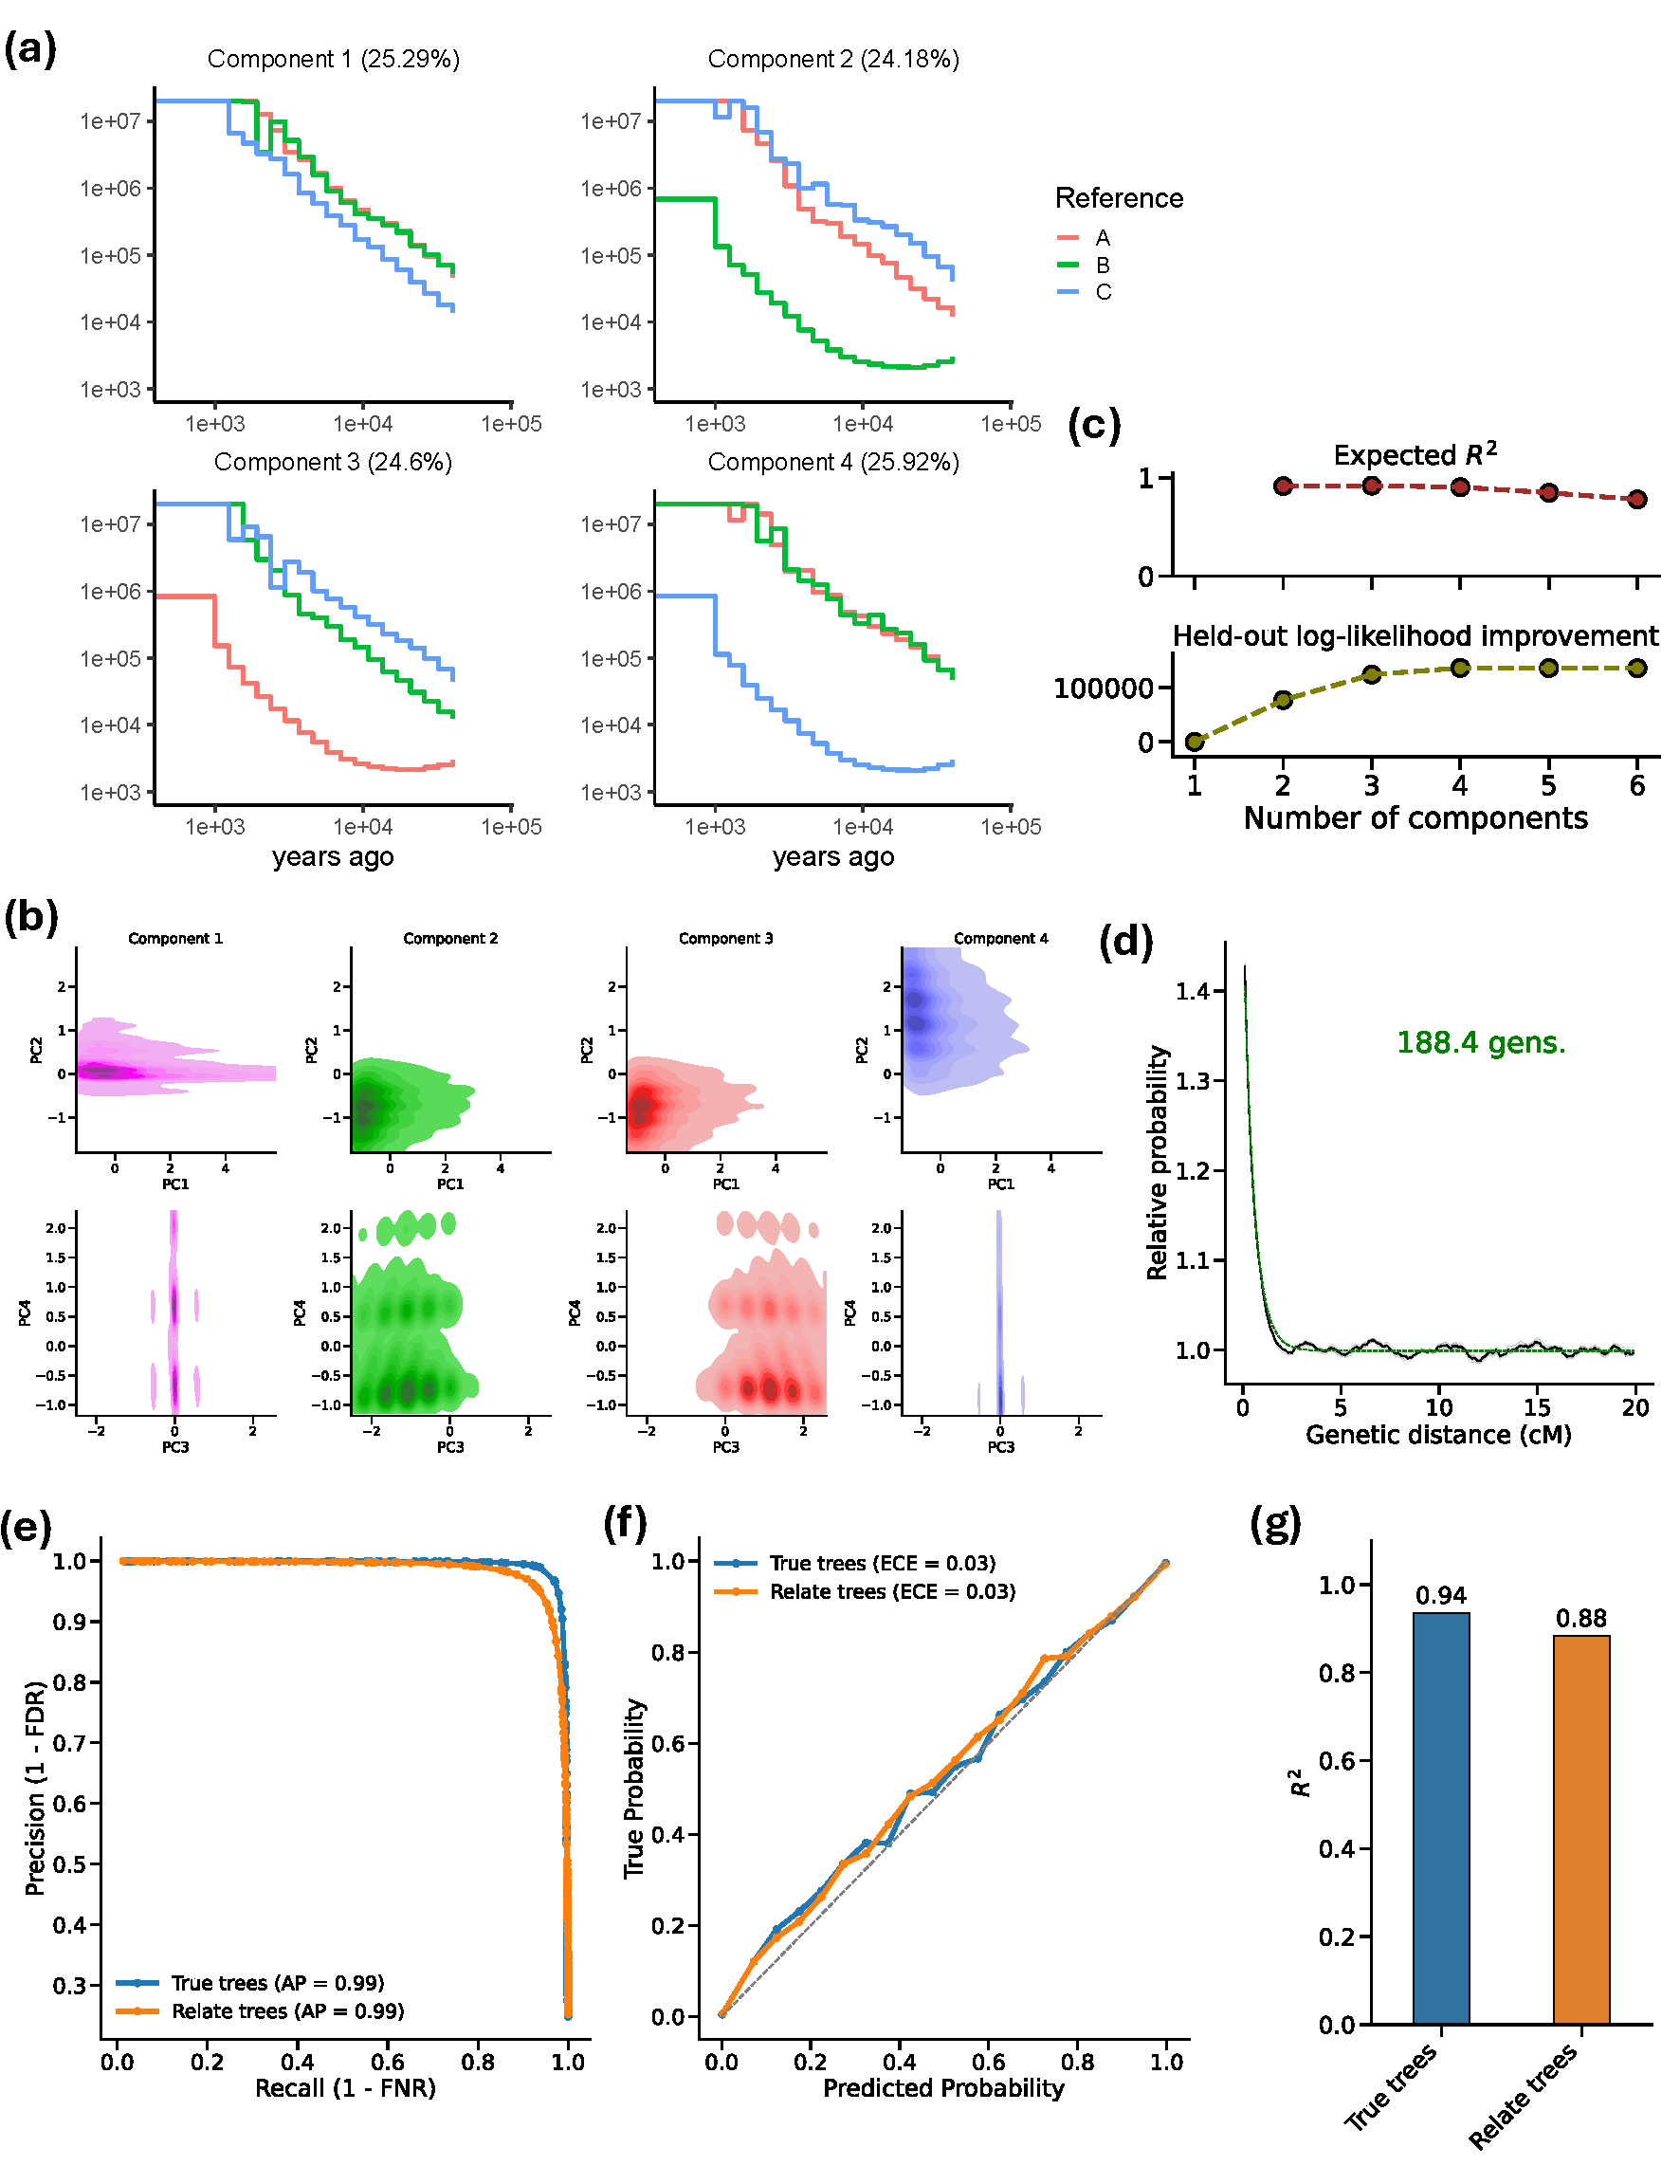
\includegraphics[width=\linewidth]{figures/gb_sims/gb_sim_4way_ghost.pdf}
    \captionsetup{width=\textwidth+3cm}     \caption{
    \footnotesize
    \textbf{Decomposing focal individuals in the four-way admix simulation with absence of one source population.} (a) Inferred inverse coalescence rates and proportions: each line represents inverse coalescence rate profiles with a reference population. (b) PCA visualization of the coalescence count and opportunity matrix derived from the genealogies plotted separately for each component. (c) Expected coefficient of determination and held-out log-likelihood improvement with varying number of components. (d) Coancestry curve for normalized joint probability of component 1 and the inferred admixture dates (in generations). (e) Precision-recall curves, (f) Calibration curves, and (g) Prediction $R^2$ for inferred local ancestry compared to the simulated ground truth, where inference was done using true trees or Relate trees. The PCA visualization in (b) is based on a KDE plot with a threshold of 0.05, and binary local ancestry estimates are obtained by thresholding the inferred posteriors at 0.5.
    }
    \label{fig:gb_sim_four_ghost}
\end{figure}


\clearpage

\subsection{Denisovan-like Introgression into Papuans}

%% explain the simulation
%% with denisovan
%% without denisovan
%% comparison with skov 
%% add ablations on hmm vs no hmm, 

We emulated the archaic introgression of Denisovan ancestry in modern-day Papuans by simulating an admixture event that occurred approximately 44,000 years ago, with an admixture proportion of 5\% (see Figure \ref{fig:sim1}b). The simulation parameters are from \cite{skov2018detecting}, and further details can be found in Section \ref{sec:ch2-gb-sim-design}. For our analysis, we simulated 25 Papuan-like individuals, 25 Mbuti-like individuals (representing African ancestry), and a Denisovan-like ancient sample. We focused on chromosomes 1 through 5 for our analysis. Our objective was to decompose the Papuan individuals' ancestry both with and without access to the Denisovan sample, aiming to accurately identify Denisovan segments and admixture within Papuans. Similar to our previous simulation of a four-way recent admixture, we primarily applied our method to trees inferred from genetic variation data via Relate, assuming a constant mutation rate of $1.25 \times 10^{-8}$. Finally, we focused only on coalescence events occurring from 10,000 to $1{,}000$,000 years for this analysis.

We begin our analysis by assuming we have access to one ancient Denisovan sample. We decompose five out of the 25 Papuan individuals, assuming two distinct components. As with the previous simulation, we randomly initialize the parameters and fit the EM algorithm for 200 iterations until the log-likelihood converges. The converged components reveal a major component, contributing around 95.85\% to the local ancestry, and a minor component contributing 4.15\% (see Figure \ref{fig:gb_sim_deni_nonghost}a). The inverse coalescence rates (ICRs) characterizing these components differ significantly. Component 1 demonstrates a slower coalescence rate with the ancient Denisovan sample and a relatively faster coalescence with the modern Mbuti samples. In contrast, component 2 exhibits a very fast coalescence rate with Denisovans but slower coalescence with modern Mbuti and Papuan samples. It is important to note that the most striking difference between the two components is the vastly accelerated coalescence with Denisovans in the minority group, up to $1{,}000 \times$ faster compared to the majority group. However, there is also a substantial difference in coalescence with modern groups, which we will leverage to decompose the ancestry without access to the ancient Denisovan sample.

The clusters were distinguishable using the top four principal components (PCs) of the coalescence count and opportunity matrices (see Figure \ref{fig:gb_sim_deni_nonghost}b). Further evaluation based on the expected coefficient of determination and held-out log-likelihood indicated that two components provided the best fit to the data, with diminishing returns in held-out log-likelihood beyond four components (see Figure \ref{fig:gb_sim_deni_nonghost}c). We also accurately dated the admixture event to $1{,}546.7$ generations, or $44{,}854.3$ years, using coancestry curves (see Figure \ref{fig:gb_sim_deni_nonghost}d). Finally, we assessed the accuracy and calibration of our local ancestry inference by comparing it with the simulated ground truth and HMMIX, a recent HMM-based method tailored to find archaic introgression such as this one \cite{skov2018detecting}, demonstrating strong correlation with the ground truth, surpassing HMMIX, and showing low calibration error (see Figure \ref{fig:gb_sim_deni_nonghost}e-g).

\begin{figure}[h!]
    \centering
    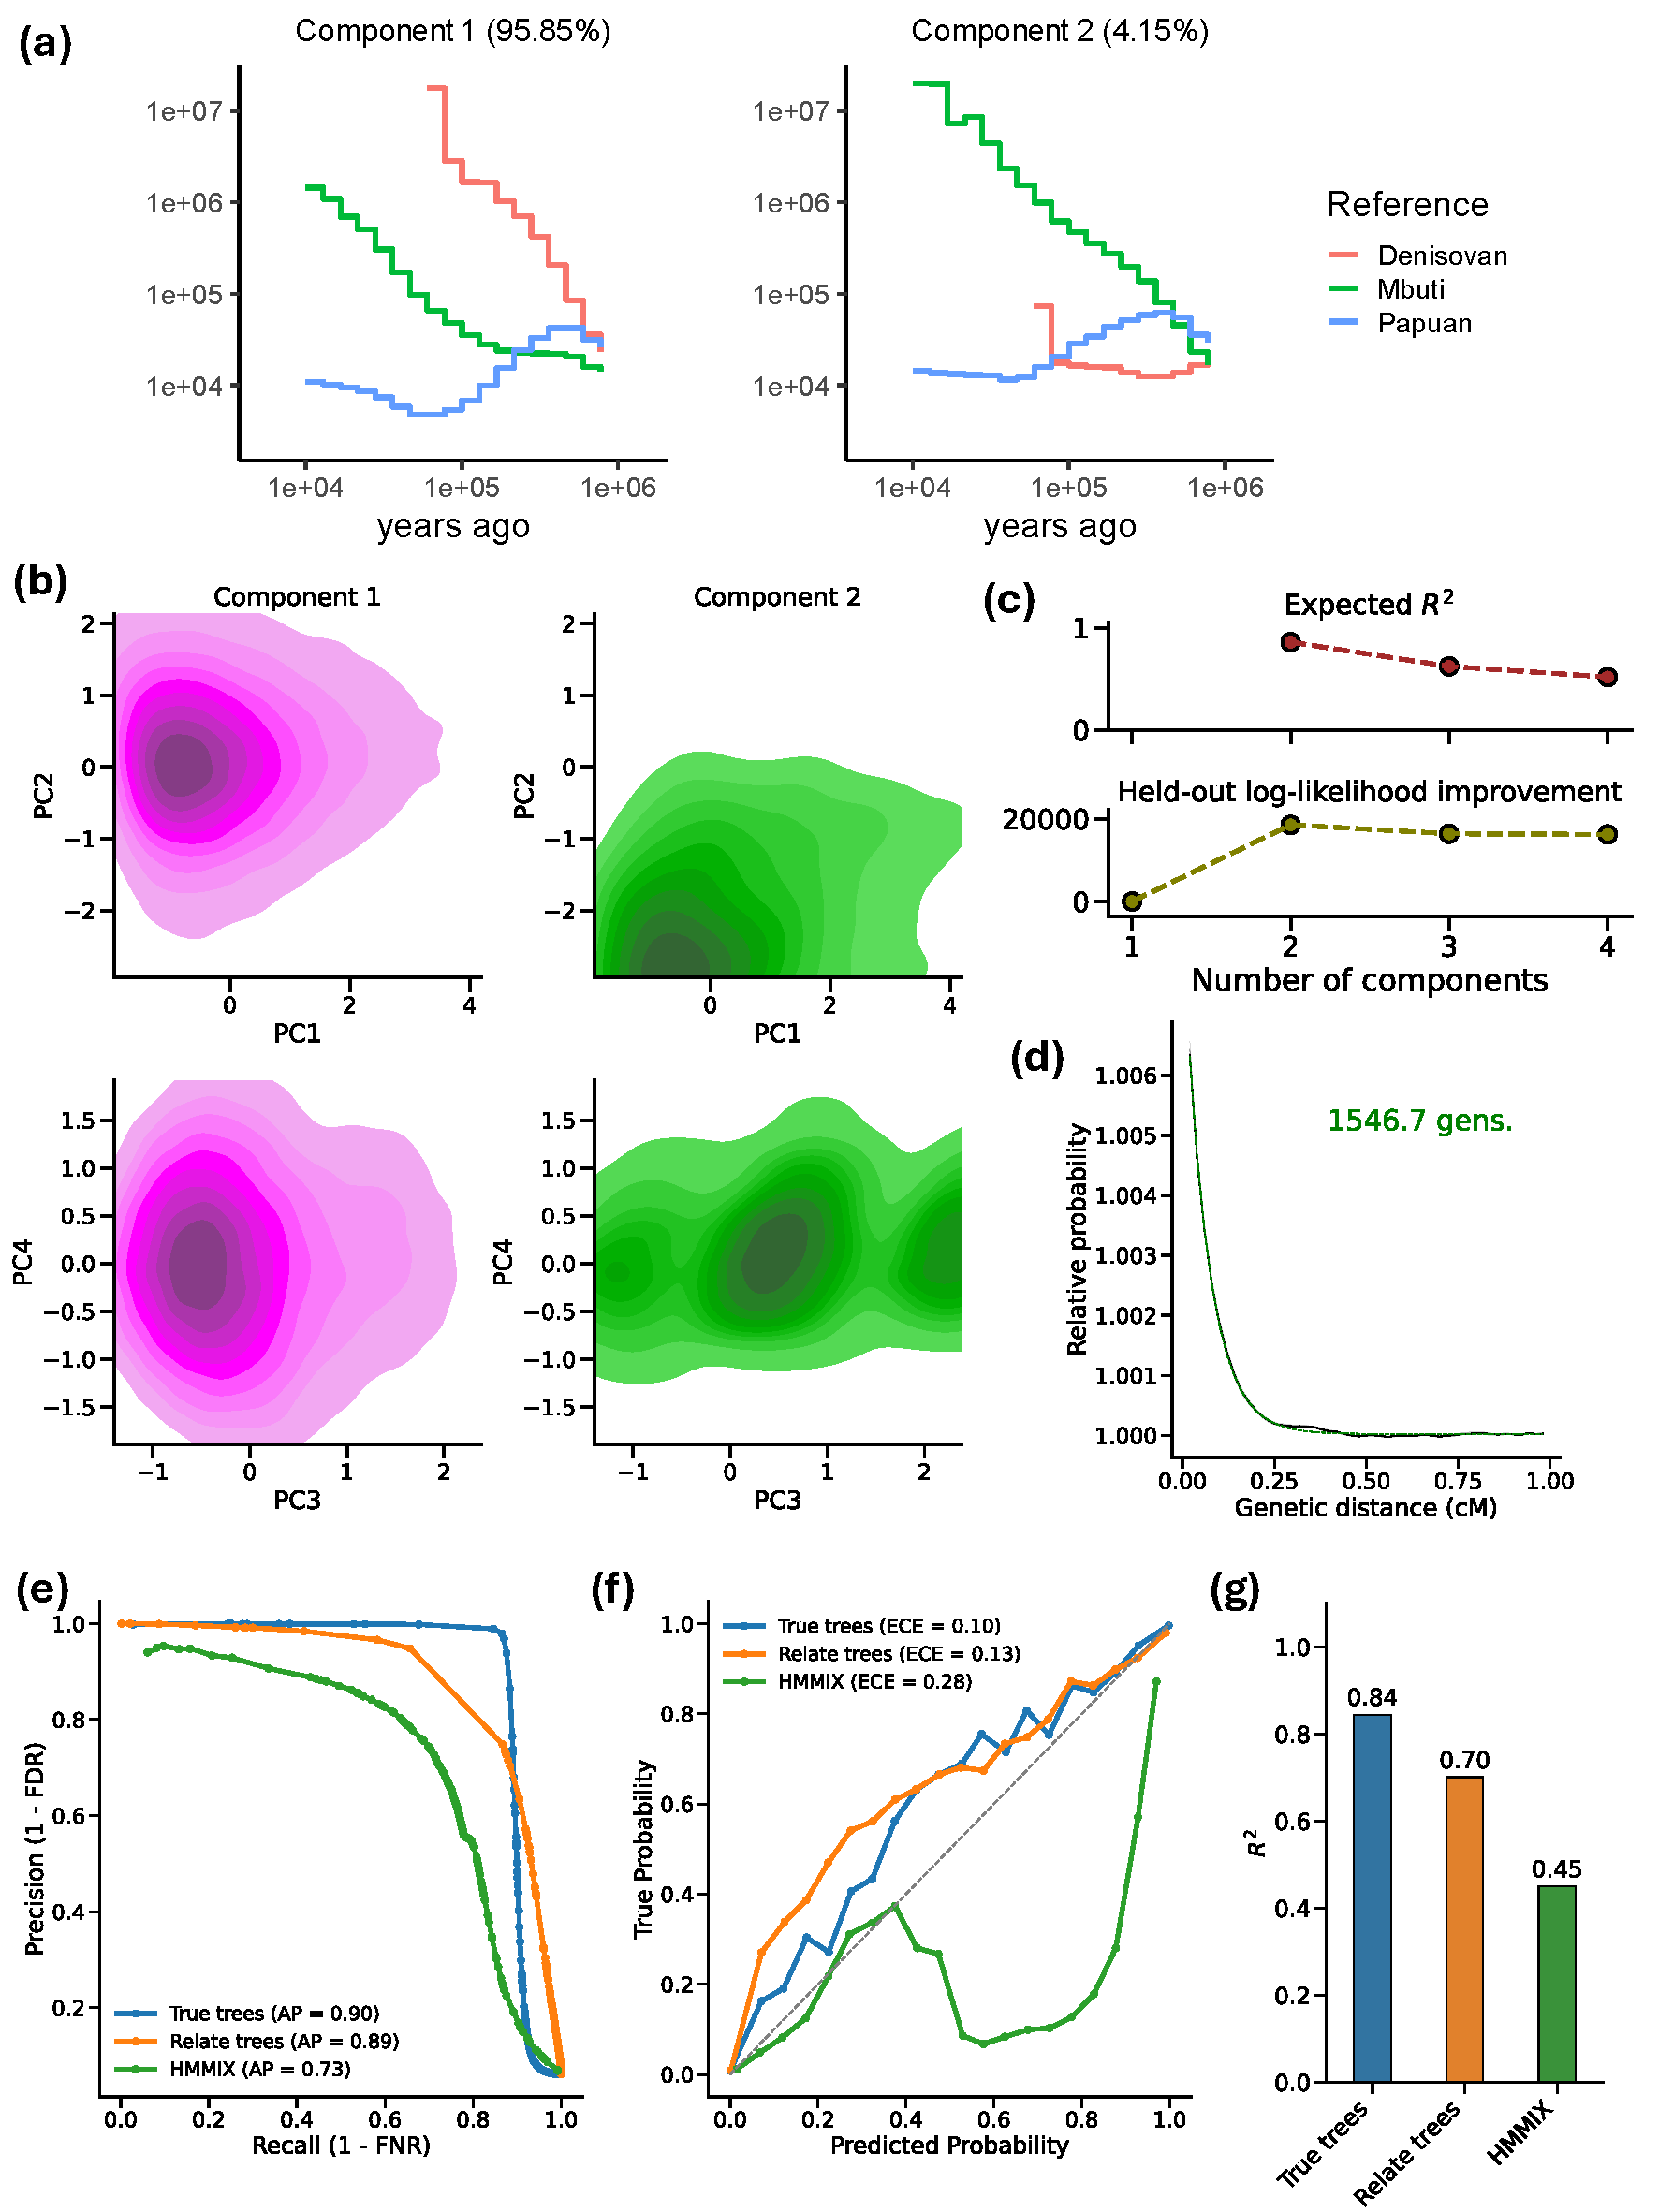
\includegraphics[width=\linewidth]{figures/gb_sims/gb_sim_deni_nonghost.pdf}
    \captionsetup{width=\textwidth+3cm}     \caption{
    \footnotesize
    \textbf{Decomposing Papuan individuals in simulations with Mbuti and Denisovans as additional references.} (a) Inferred inverse coalescence rates and proportions: each line represents inverse coalescence rate profiles with a reference population. (b) PCA visualization of the coalescence count and opportunity matrix derived from the genealogies plotted separately for each component. (c) Expected coefficient of determination and held-out log-likelihood improvement with varying number of components. (d) Coancestry curve for normalized joint probability of component 1 and the inferred admixture dates (in generations).  (e) Precision-recall curves, (f) Calibration curves, and (g) Prediction $R^2$ for inferred local ancestry compared to the simulated ground truth, where inference was done using true trees or Relate trees. The PCA visualization in (b) is based on a KDE plot with a threshold of 0.05, and binary local ancestry estimates are obtained by thresholding the inferred posteriors at 0.5.
    }
    \label{fig:gb_sim_deni_nonghost}
\end{figure}

Next, we removed the Denisovan samples from our analysis and decomposed the same Papuan individuals into two components. In this scenario, the Denisovan ancestry in Papuans can be thought of as a ghost population. Our method converged on two components, contributing approximately 95.9\% and 4.1\% to the local ancestry, respectively (see Figure \ref{fig:gb_sim_deni_ghost}a). The ICRs of the minor component closely matched those of the minor component from the earlier analysis that included the Denisovan sample, showing slower coalescence with Mbuti and Papuans (see Figure \ref{fig:gb_sim_deni_nonghost}a). Similar to the run with access to the Denisovan genome, we performed PCA visualization (Figure \ref{fig:gb_sim_deni_ghost}b), evaluation of the number of clusters (Figure \ref{fig:gb_sim_deni_ghost}c), coancestry curve dating (Figure \ref{fig:gb_sim_deni_ghost}d), and accuracy and calibration of local ancestry inference (Figures \ref{fig:gb_sim_deni_ghost}e-g). To verify that the minor component indeed represents Denisovan ancestry, we compared the local ancestry inferred using GhostBuster with the simulated ground truth and found a high degree of correlation ($R^2 = 0.63$), surpassing HMMIX \cite{skov2018detecting}.

\begin{figure}[h!]
    \centering
    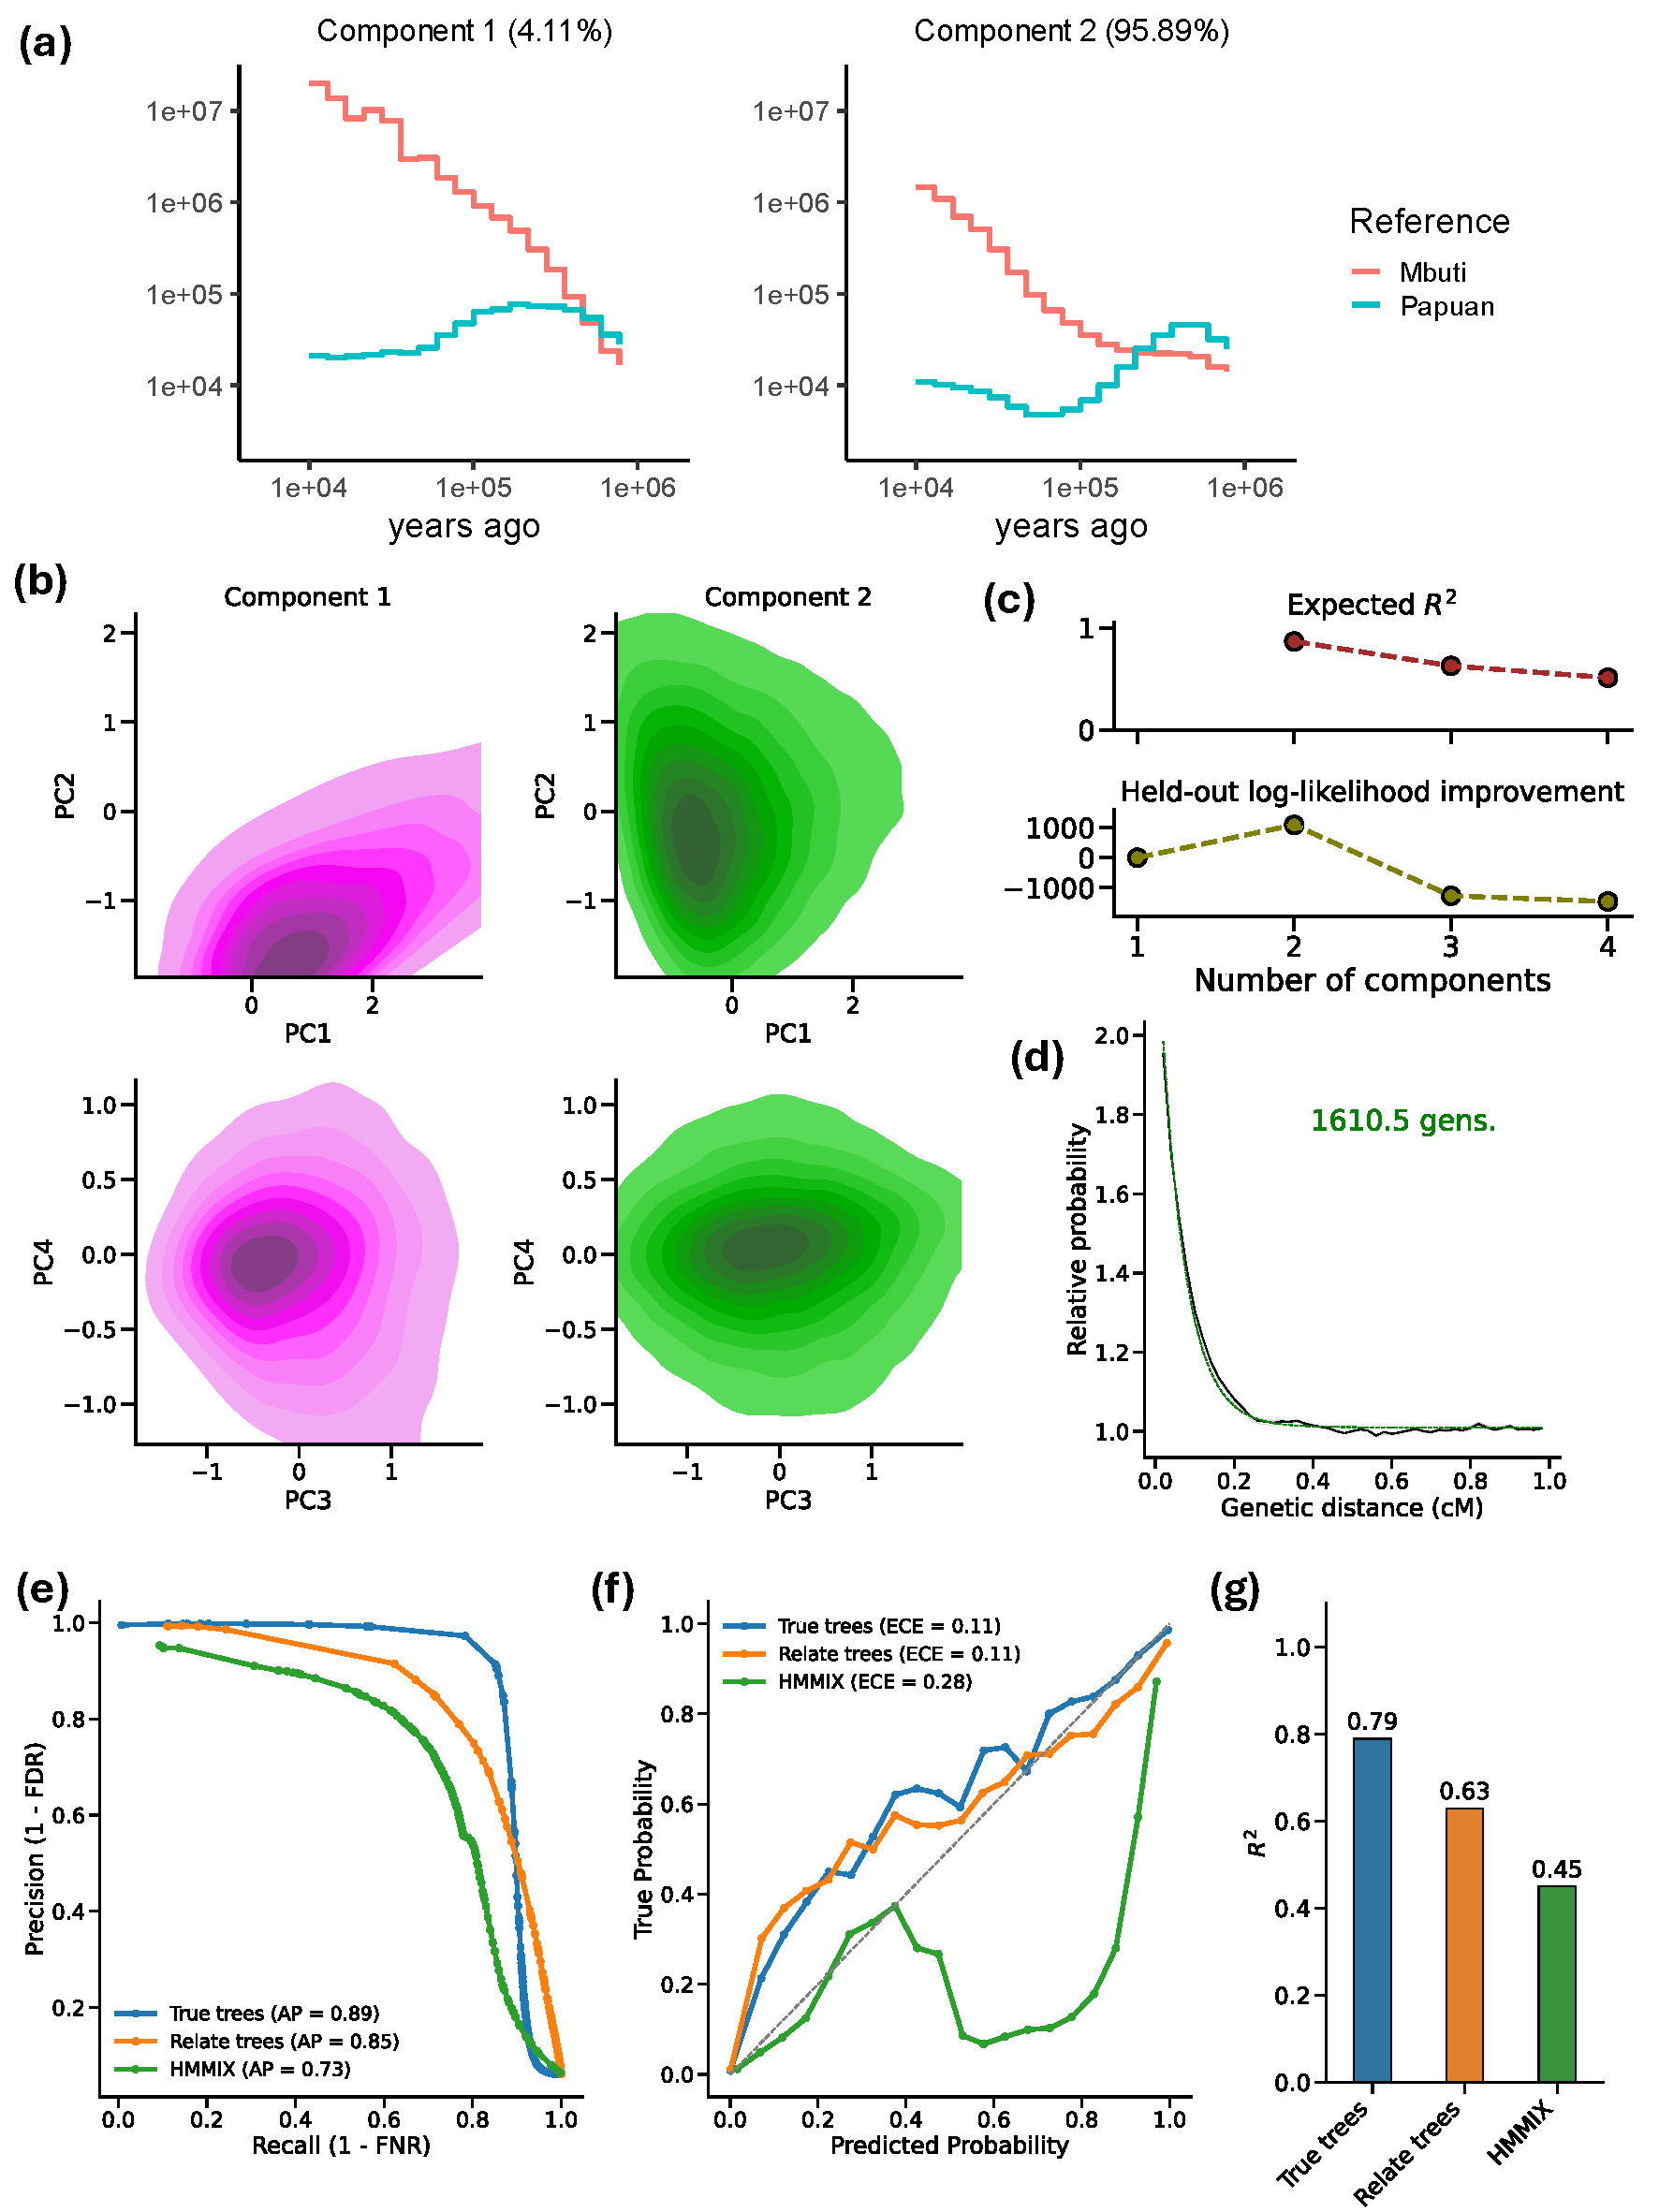
\includegraphics[width=\linewidth]{figures/gb_sims/gb_sim_deni_ghost.pdf}
    \captionsetup{width=\textwidth+3cm}     \caption{
    \footnotesize
    \textbf{Decomposing Papuan individuals in simulations with only Mbuti as additional references.} (a) Inferred inverse coalescence rates and proportions: each line represents inverse coalescence rate profiles with a reference population. (b) PCA visualization of the coalescence count and opportunity matrix derived from the genealogies plotted separately for each component. (c) Expected coefficient of determination and held-out log-likelihood improvement with varying number of components. (d) Coancestry curve for normalized joint probability of component 1 and the inferred admixture dates (in generations). (e) Precision-recall curves, (f) Calibration curves, and (g) Prediction $R^2$ for inferred local ancestry compared to the simulated ground truth, where inference was done using true trees or Relate trees. The PCA visualization in (b) is based on a KDE plot with a threshold of 0.05, and binary local ancestry estimates are obtained by thresholding the inferred posteriors at 0.5.
    }
    \label{fig:gb_sim_deni_ghost}
\end{figure}

In order to test the robustness and false-positive rate of our method, we attempted to decompose five Mbuti individuals in the same simulation. The Mbuti individuals are panmictic, with no simulated population structure or admixture. When we forced GhostBuster to find two components for relate trees, it identified two components with varying coalescence rates with Papuans. However, these components were not clearly separated in the PC plots. In terms of held-out log-likelihood, the two-component solution offered only a slight improvement compared to a single-component model. Moreover, the histogram of the local ancestry posteriors and the expected coefficient of determination, with $R = 0.49$, both suggest that the local ancestry inferred is highly uncertain in this case. Additionally, dating this event using coancestry curves inferred an admixture date of around $2{,}800$ generations ($81{,}200$ years), which is older than the Mbuti and Papuan split time in this simulation, raising suspicion. Thus, while it is possible to fit a two-component model, it does not necessarily provide compelling evidence for admixture. It is therefore crucial to evaluate PC plots, held-out likelihood, expected coefficient of determination, and coancestry dating along with other sources of evidence in real-data analyses to be more confident about the presence of gene flow or admixture.

\begin{figure}[h!]
    \centering
    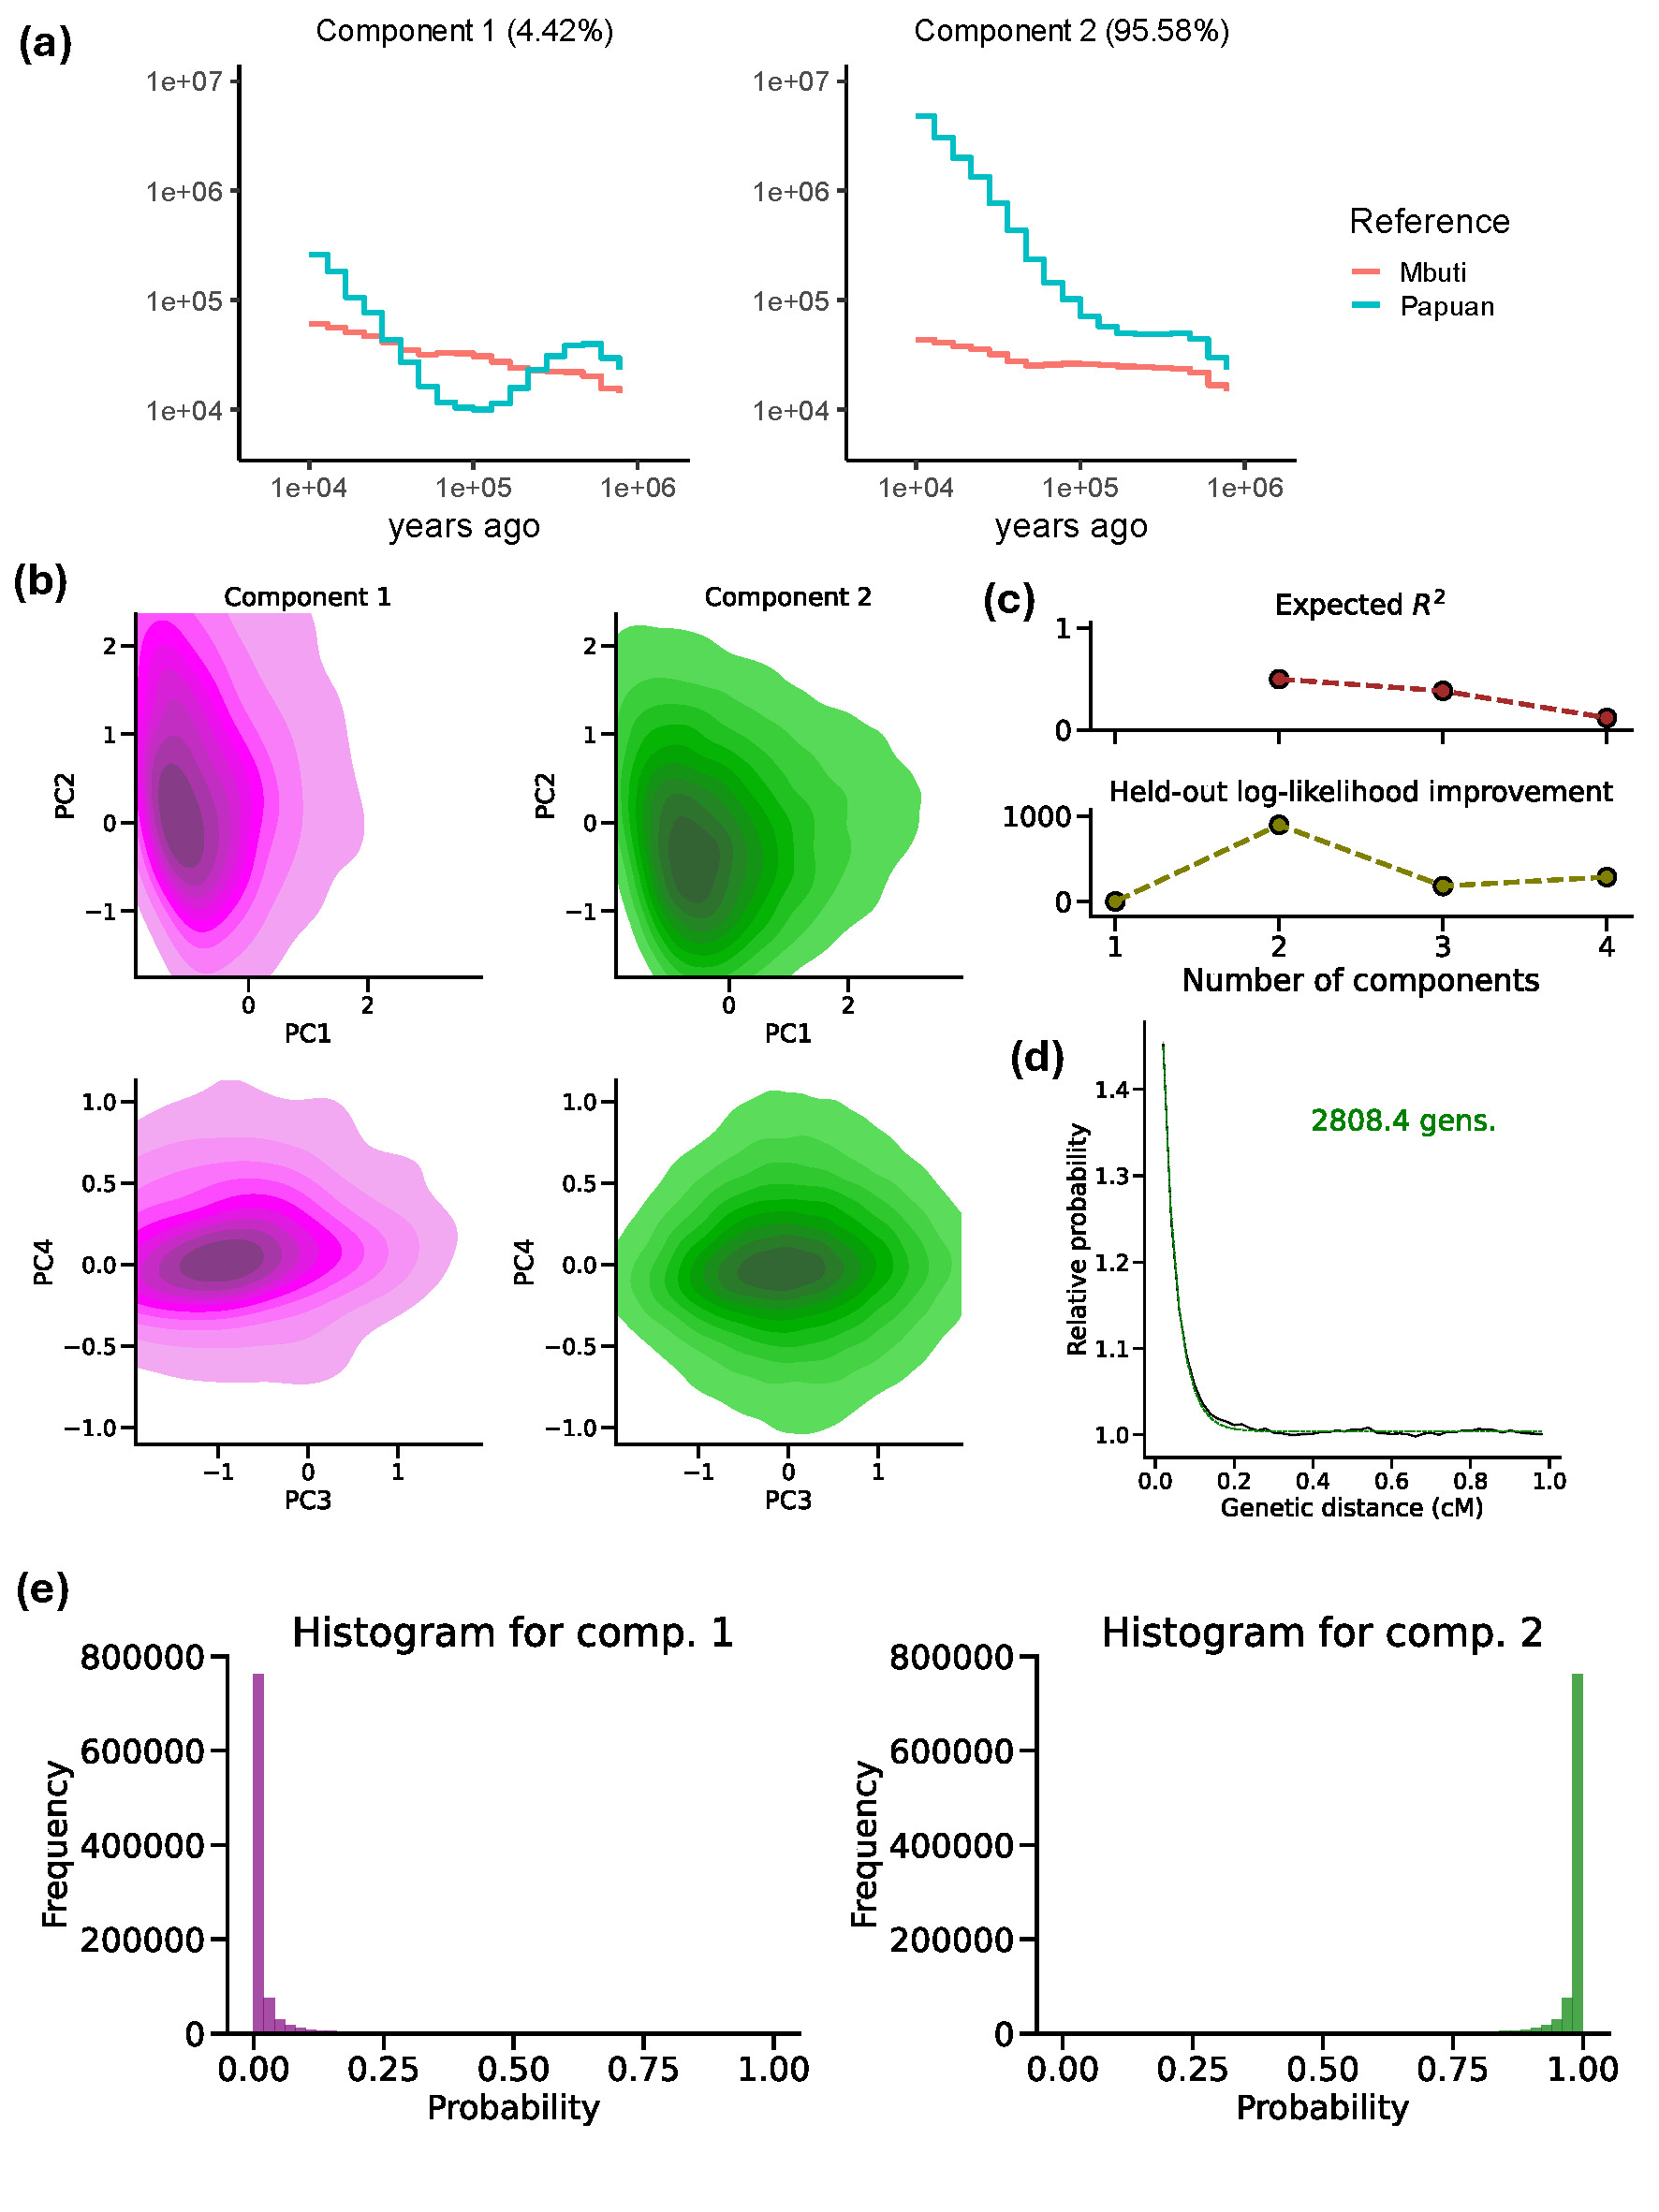
\includegraphics[width=\linewidth]{figures/gb_sims/gb_sim_deni_noadmix.pdf}
    \captionsetup{width=\textwidth+3cm}     \caption{
    \footnotesize
    \textbf{Decomposing Mbuti individuals in simulations with Papuan as additional references.} (a) Inferred inverse coalescence rates and proportions: each line represents inverse coalescence rate profiles with a reference population. (b) PCA visualization of the coalescence count and opportunity matrix derived from the genealogies plotted separately for each component. (c) Expected coefficient of determination and held-out log-likelihood improvement with varying number of components. (d) Coancestry curve for normalized joint probability of component 1 and the inferred admixture dates (in generations). (e) Histogram of the inferred local ancestry posteriors. The PCA visualization in (b) is based on a KDE plot with a threshold of 0.05, and binary local ancestry estimates are obtained by thresholding the inferred posteriors at 0.5.
    }
    \label{fig:gb_sim_deni_noadmix}
\end{figure}

\clearpage

\section{Identifying several recent admixtures accurately}
\label{sec:ch2-gb-real}

Haplotype-based methods like Alder \cite{loh2013inferring}, Globetrotter \cite{hellenthal2014genetic}, and Mosaic \cite{salter2019fine} have been instrumental in inferring recent admixture events, particularly those occurring less than 2,000 years ago. We focus on several well-documented, recently admixed populations from the Human Genome Diversity Project (HGDP), namely the Hazara, Bedouin, and Maya. Each of these populations has undergone two-way admixture events within the past few thousand years, which have been reliably detected by previous methods. Our objective is to decompose the ancestry of individuals from these populations using GhostBuster and to compare the local ancestry with results from other haplotype-based methods.

We begin by decomposing the ancestry of Hazara individuals from the HGDP, who have been shown in previous studies to result from recent admixture between groups similar to modern-day Pathans in South Asia and Mongols in East Asia \cite{hellenthal2014genetic,salter2019fine}. Using all populations in our HGDP + $1{,}000$GPA dataset (as described in Section \ref{sec:ch2-gb-data}), we fit two components to decompose the ancestry of the five Hazara individuals from chromosome one to five. We focused on coalescence events within the last 10,000 years, dividing the time scale into 10 logarithmically spaced epochs. Our analysis revealed that the Hazara individuals could be decomposed into two components, each contributing roughly 50\% to the overall ancestry. The inverse coalescence rates (ICRs) indicate that component 1 is closely related to East Asian groups, while component 2 is more closely aligned with South Asian groups—consistent with previous findings using Globetrotter and Mosaic (see Figure \ref{fig:gb_hazara}a). The two components separated clearly in the PC plots (see Figure \ref{fig:gb_hazara}b). Moreover, two components provided the best fit with high expected coefficient of determination and held-out likelihood improvement (see Figure \ref{fig:gb_hazara}c). The coancestry curves inferred admixture dates of around $26.2$ generations or $733.6$ years, assuming 28 years per generation (see Figure \ref{fig:gb_hazara}d). To further validate our results, we compared the local ancestry estimates from our method with those obtained using Mosaic, which was run using genotyped variants and all reference populations in HGDP. We found that the local ancestry was highly correlated between the two methods, with a mean correlation of $0.87$ (see Figure \ref{fig:gb_hazara}e). Potential differences in local ancestry estimates may be attributed to additional steps in Mosaic, such as correction for phasing, which are not present in our method.

\begin{figure}[h!]
    \centering
    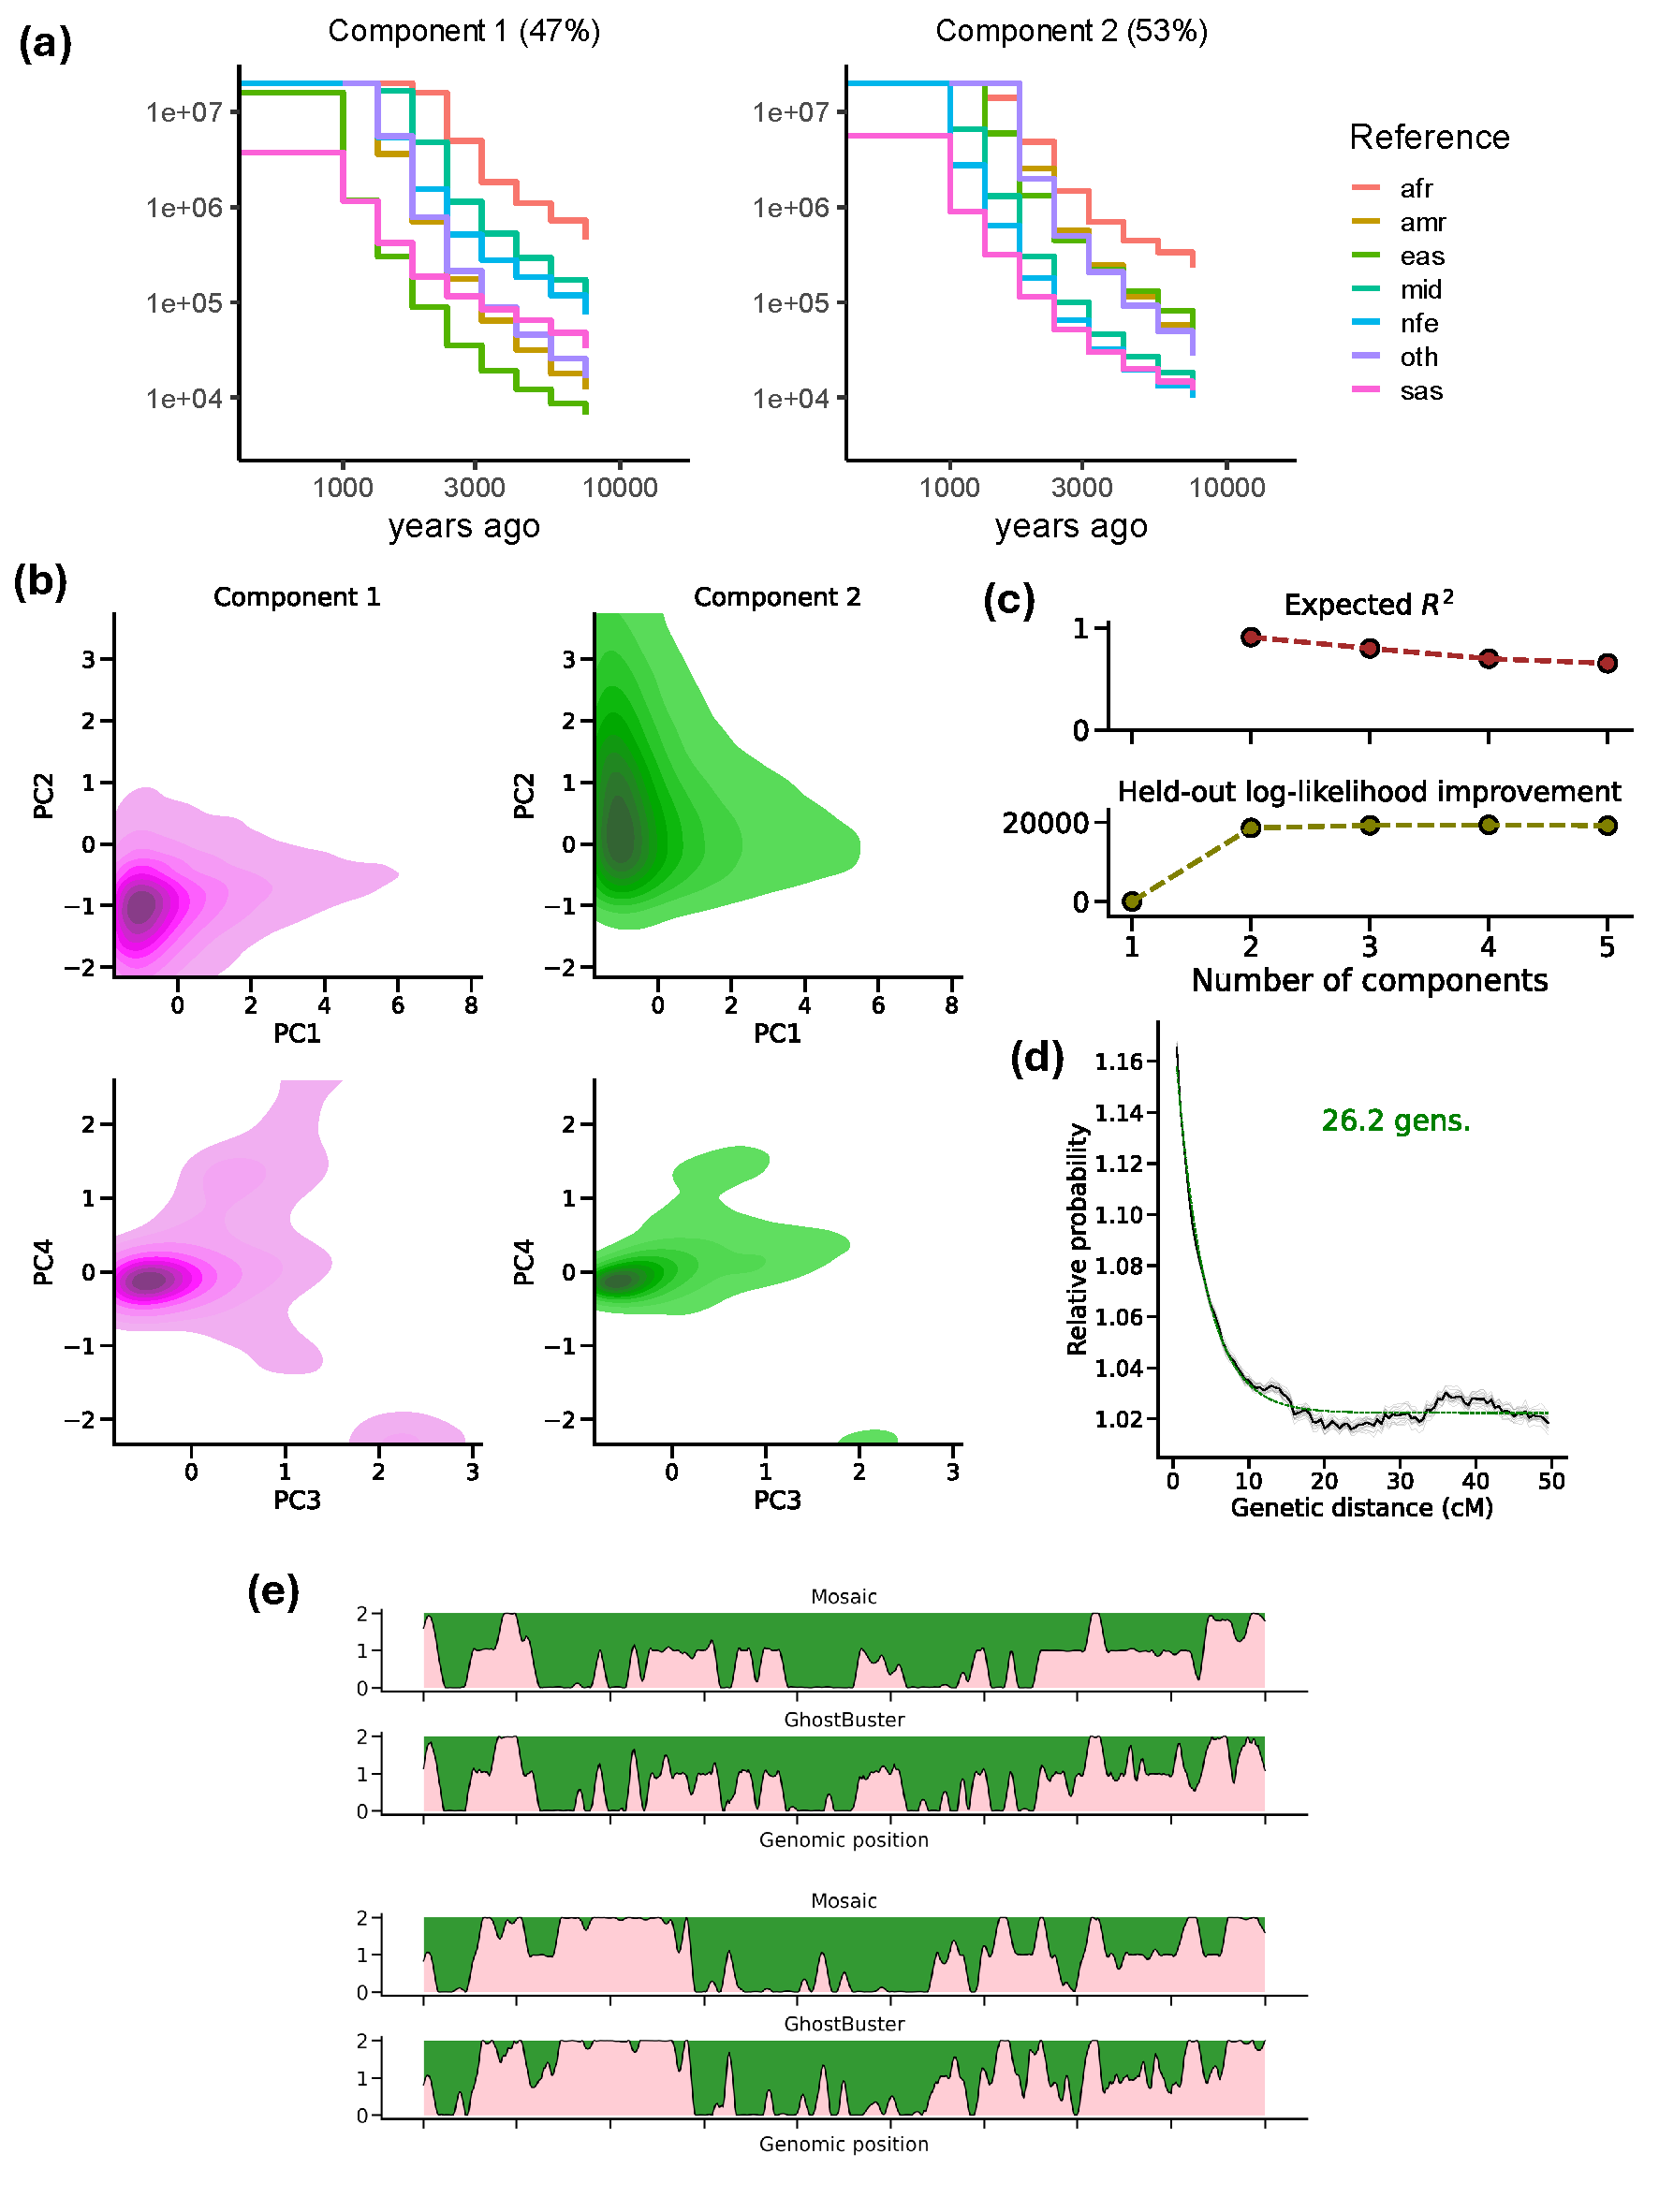
\includegraphics[width=\linewidth]{figures/gb_sims/gb_real_hazara.pdf}
    \captionsetup{width=\textwidth+3cm}     \caption{
    \footnotesize
    \textbf{Decomposing Hazara individuals in Human Genome Diversity Project.} (a) Inferred inverse coalescence rates and proportions: each line represents inverse coalescence rate profiles with a reference population. (b) PCA visualization of the coalescence count and opportunity matrix derived from the genealogies plotted separately for each component. (c) Expected coefficient of determination and held-out log-likelihood improvement with varying number of components. (d) Coancestry curve for normalized joint probability of component 1 and the inferred admixture dates (in generations). (e) Local ancestry inference for GhostBuster vs. Mosaic. The PCA visualization in (b) is based on a KDE plot with a threshold of 0.05, and binary local ancestry estimates are obtained by thresholding the inferred posteriors at 0.5. The diploid local ancestry in (e) is based on chromosome 1 for HGDP samples HGDP00102 and HGDP00103.
    }
    \label{fig:gb_hazara}
\end{figure}

We conducted similar analyses for other populations in the HGDP, including the Bedouin, who have a well-documented history of European and African admixture within the last 40 generations. Our findings reveal two components: a major component, comprising 90\%, closely aligned with Middle Eastern and European groups, and a minor component more closely related to sub-Saharan African groups (see Figure~\ref{fig:gb_bedouin}a). The PC plots effectively distinguish between these ancestries (see Figure~\ref{fig:gb_bedouin}b), and the coancestry curves suggest an admixture date of approximately 36.6 generations or 1,024.8 years (see Figure~\ref{fig:gb_bedouin}d). Similar to our analysis of the Hazara, the local ancestry inferred with GhostBuster shows a high correlation with that inferred using Mosaic, with a mean local ancestry correlation of 0.86 (see Figure~\ref{fig:gb_bedouin}e).

\begin{figure}[h!]
    \centering
    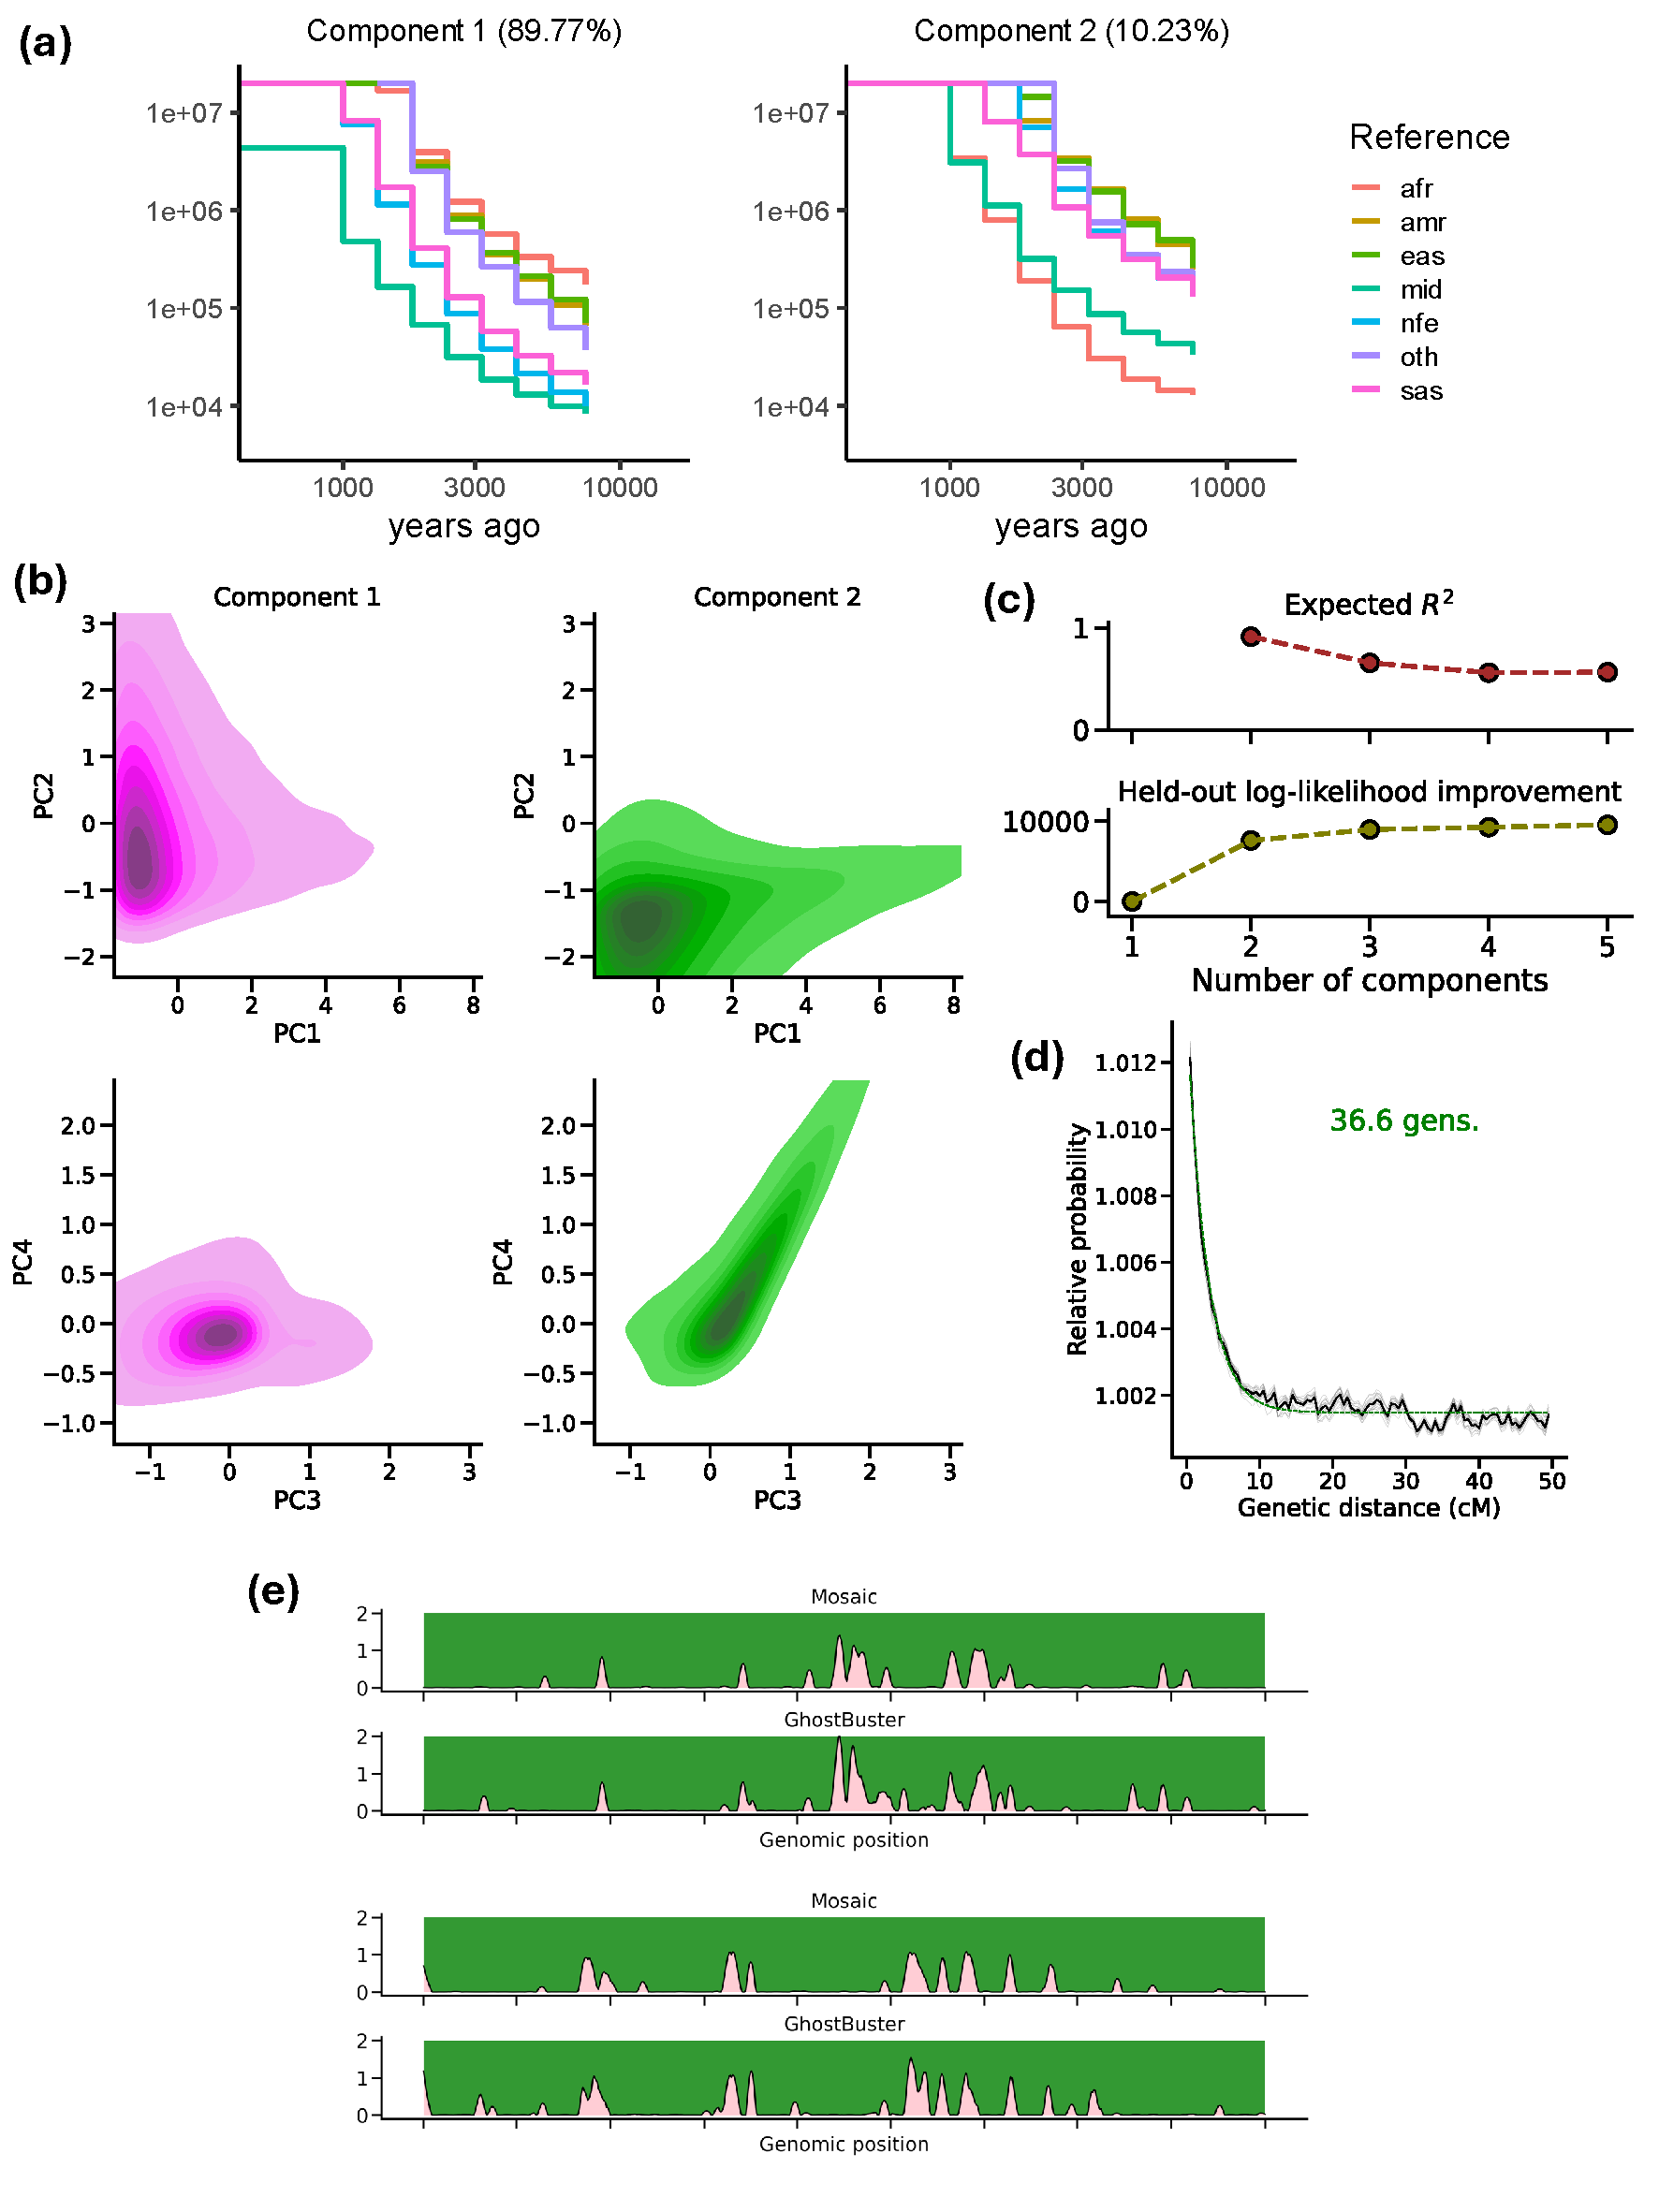
\includegraphics[width=\linewidth]{figures/gb_sims/gb_real_bedouin.pdf}
    \captionsetup{width=\textwidth+3cm}     \caption{
    \footnotesize
    \textbf{Decomposing Bedouin individuals in Human Genome Diversity Project.} (a) Inferred inverse coalescence rates and proportions: each line represents inverse coalescence rate profiles with a reference population. (b) PCA visualization of the coalescence count and opportunity matrix derived from the genealogies plotted separately for each component. (c) Expected coefficient of determination and held-out log-likelihood improvement with varying number of components. (d) Coancestry curve for normalized joint probability of component 1 and the inferred admixture dates (in generations). (e) Local ancestry inference for GhostBuster vs. Mosaic. The PCA visualization in (b) is based on a KDE plot with a threshold of 0.05, and binary local ancestry estimates are obtained by thresholding the inferred posteriors at 0.5. The diploid local ancestry in (e) is based on chromosome 1 for HGDP samples HGDP00607 and HGDP00608.
    }
    \label{fig:gb_bedouin}
\end{figure}

Finally, we analyzed Maya individuals from Central America, who exhibit a well-documented two-way admixture between Native American and European ancestries, largely resulting from European colonization. We identified two components: the major component, comprising 86\%, is closely aligned with other Native American groups, while the minor component shows a closer relationship to European groups (see Figure~\ref{fig:gb_maya}a). The PC plots successfully separate the ancestries (see Figure~\ref{fig:gb_maya}b), and the coancestry curves estimate an admixture date of approximately 6.4 generations, or 179.2 years (see Figure~\ref{fig:gb_maya}d). As with the Hazara and Bedouin populations, the local ancestry inferred with GhostBuster showed a strong correlation with Mosaic, with a mean local ancestry correlation of 0.92 (see Figure~\ref{fig:gb_maya}e).

\begin{figure}[h!]
    \centering
    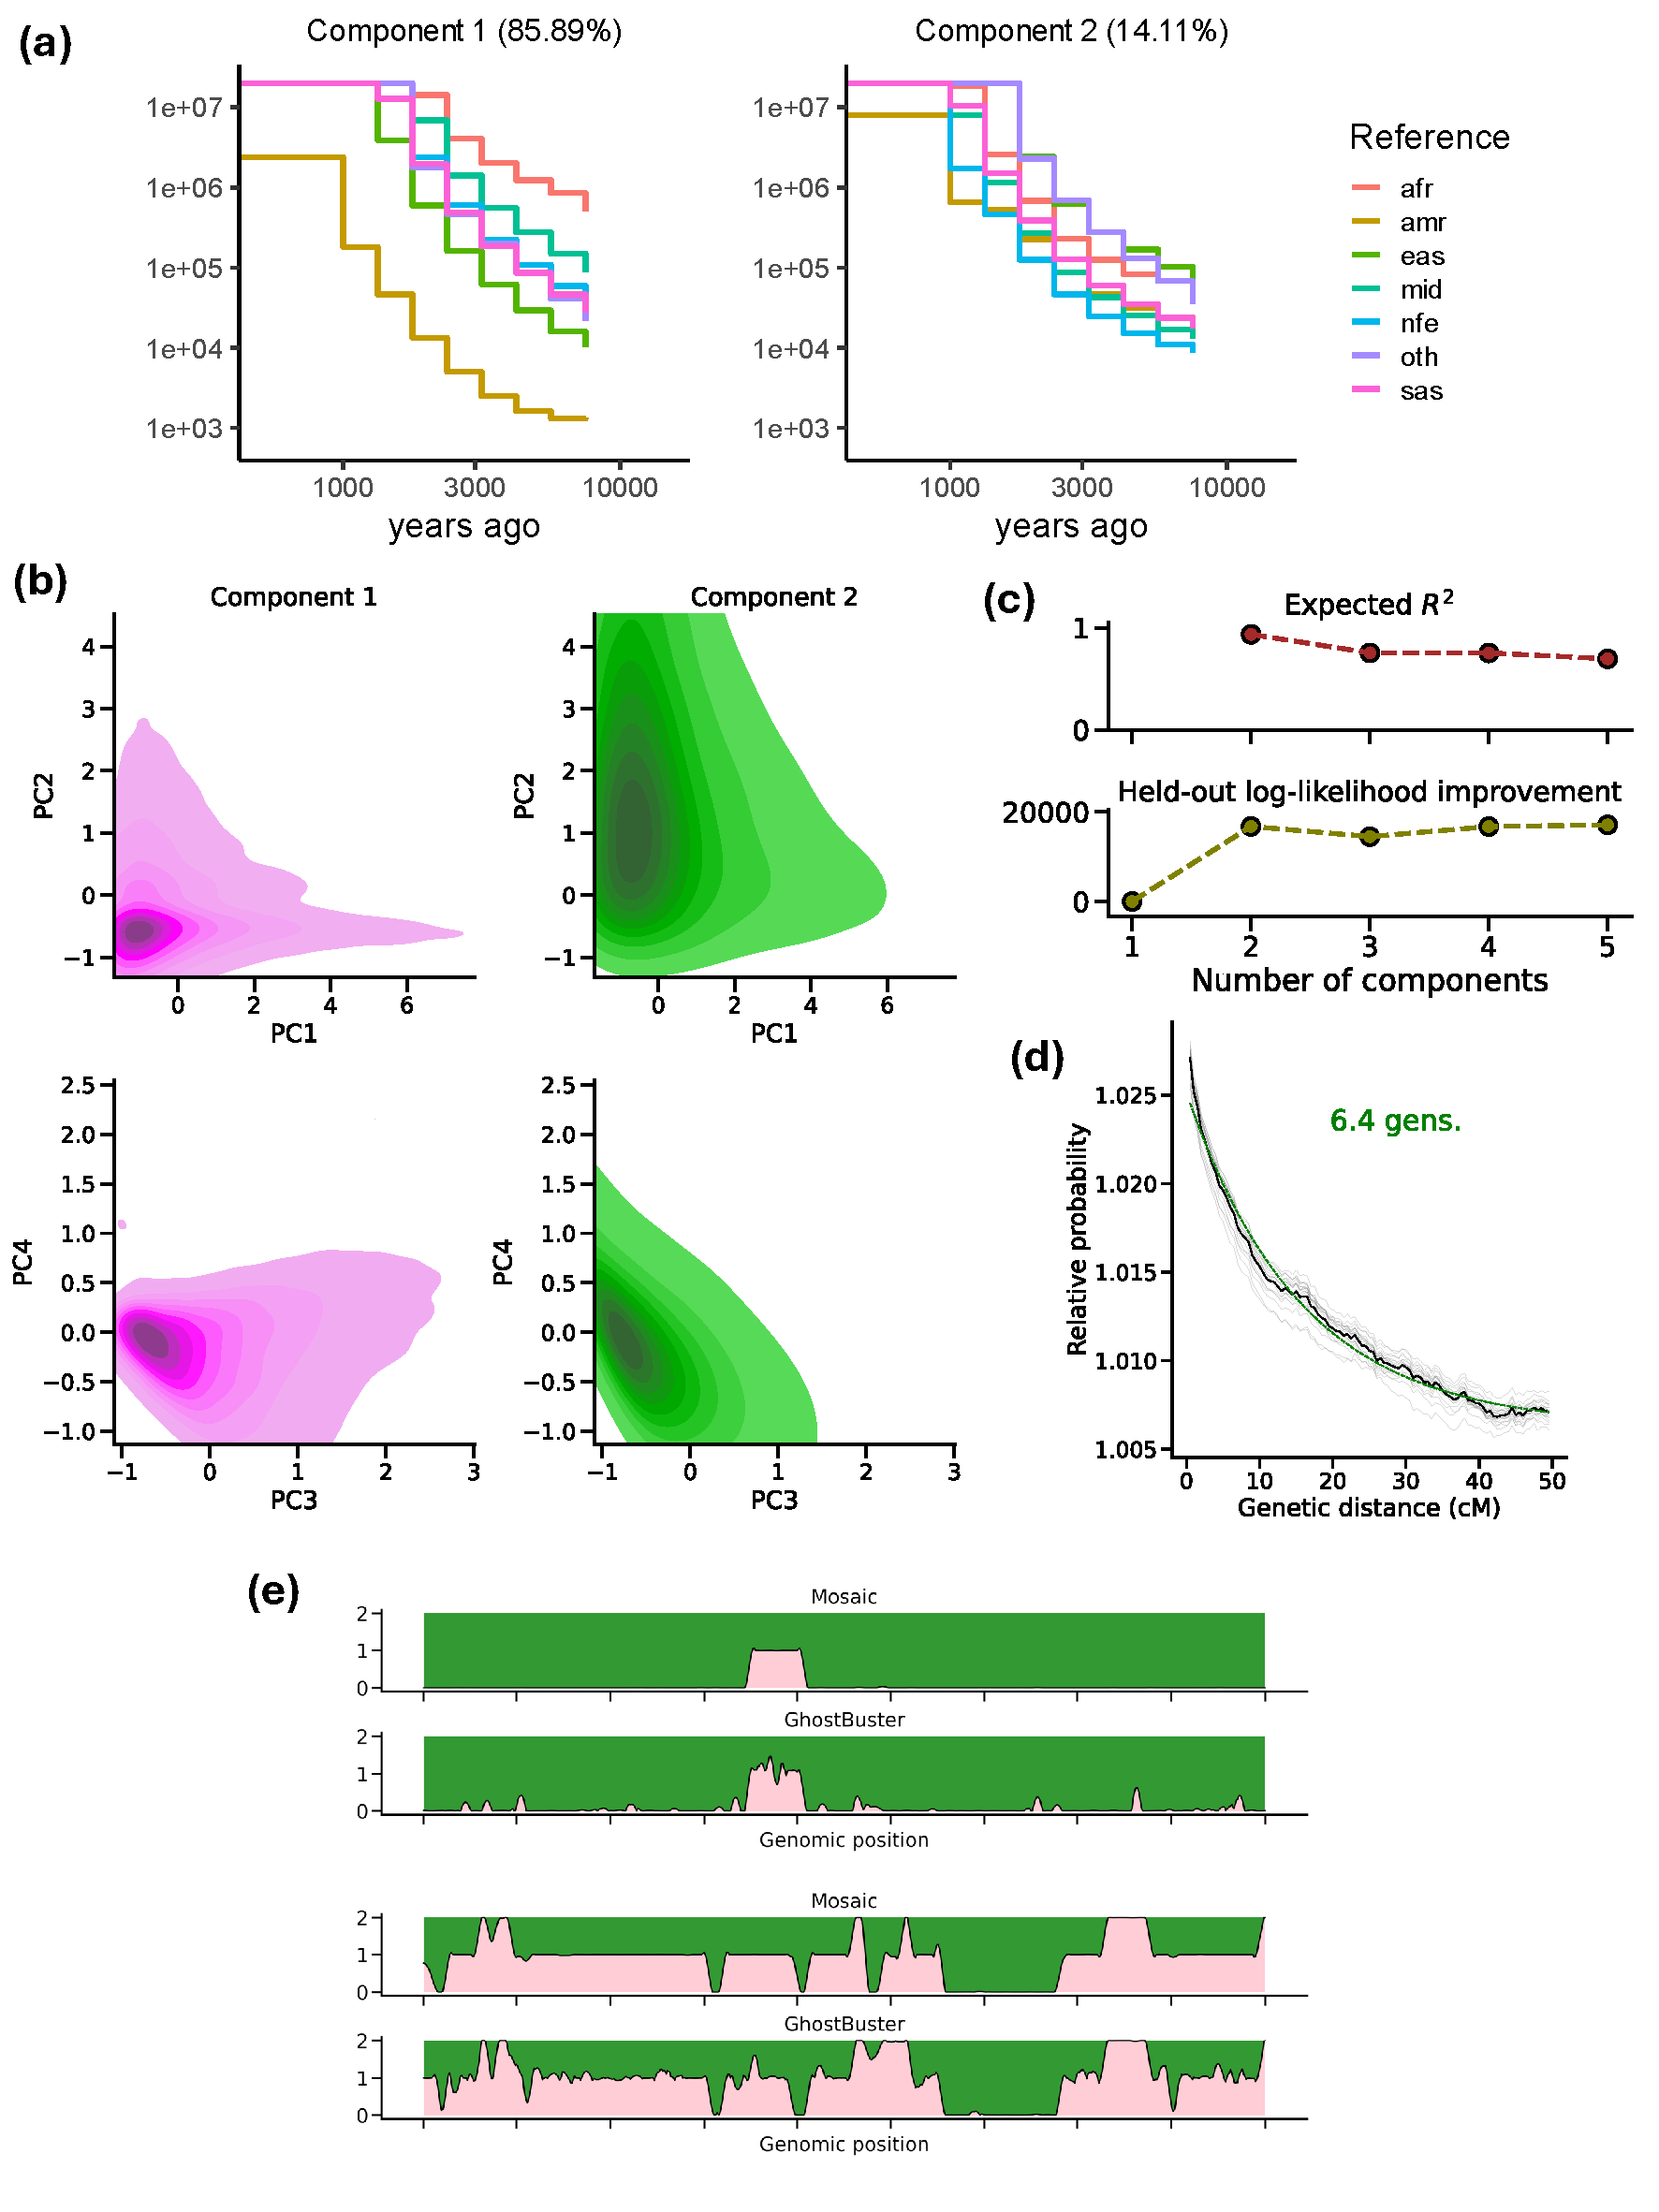
\includegraphics[width=\linewidth]{figures/gb_sims/gb_real_maya.pdf}
    \captionsetup{width=\textwidth+3cm}     \caption{
    \footnotesize
    \textbf{Decomposing Maya individuals in Human Genome Diversity Project.} (a) Inferred inverse coalescence rates and proportions: each line represents inverse coalescence rate profiles with a reference population. (b) PCA visualization of the coalescence count and opportunity matrix derived from the genealogies plotted separately for each component. (c) Expected coefficient of determination and held-out log-likelihood improvement with varying number of components. (d) Coancestry curve for normalized joint probability of component 1 and the inferred admixture dates (in generations). (e) Local ancestry inference for GhostBuster vs. Mosaic. The PCA visualization in (b) is based on a KDE plot with a threshold of 0.05, and binary local ancestry estimates are obtained by thresholding the inferred posteriors at 0.5. The diploid local ancestry in (e) is based on chromosome 1 for HGDP samples HGDP00856 and HGDP00860.
    }
    \label{fig:gb_maya}
\end{figure}

\clearpage

\section{Identifying multi-way admixture in holocene Europe}
\label{sec:ch2-gb-real-eur}

Europe's prehistory is among the most thoroughly understood, owing to the wealth of ancient DNA data, archaeological evidence, and linguistic studies conducted in the region. One of the most significant breakthroughs in ancient DNA research over the past decade has been the identification of a large-scale migration from the Steppe into Europe (and Asia), which fundamentally altered the genetic landscape of the continent over the past 5,000 years \cite{haak2015massive}. Prior to this discovery, archaeological evidence indicated the existence of only two major ancestral groups in Europe: the indigenous hunter-gatherer populations and the agricultural communities that migrated from Anatolia. However, ancient DNA studies revealed the presence of a third ancestry, which in many cases now constitutes the dominant component of modern European genomes and is also likely the origin of the Indo-European languages \cite{lazaridis2024genetic}. This third ancestry is most strongly associated with the Yamnaya people, who inhabited the Steppe region north of the Caspian Sea, in what is present-day Ukraine and Russia. The Yamnaya are thought to have lived primarily as nomadic herders and were among the earliest adopters of wheeled carts and wagons. Their influence extended to the final Neolithic cultures, such as the Corded Ware and Bell Beaker cultures, which spread throughout Europe, both culturally and genetically. See Figure \ref{fig:gb-intro}B for an illustration of this 3-way admixture in Europe.

We compiled a dataset of high-coverage ancient DNA samples corresponding to $17$ ancient Anatolian, Balkan, or Neolithic farmers, $2$ ancient Western hunter-gatherers, and one Yamnaya sample. We additionally added $5$ present-day British samples from $1{,}000$ GP, which we decomposed considering a time span from $1{,}000$ to $30{,}000$ years ago. With the abundance of ancient DNA in Europe, it is increasingly clear that most populations, including the British samples, have undergone at least two waves of admixture. The first wave, corresponding to the origin and spread of farming from Anatolia, led to the mixing of local hunter-gatherer groups with farmers from the Near East. The second wave is believed to correspond to the later large-scale Yamnaya-like ancestry from the Steppe. When we ran GhostBuster with three components, we found that each component was closer to one of the ancient groups. Component 1, contributing $12\%$, is closest to Western hunter-gatherers, component 2, contributing $45.6\%$, is closer to farmers, and component 3, explaining the remainder, is closest to Yamnaya (see Figure \ref{fig:gb_eur_3way}a). The ancestry separates in the PC plots, most strikingly for component 3 versus rest (see Figure \ref{fig:gb_eur_3way}b), and the coancestry curves suggest admixture dates of around $330$ generations for component 1, and $262$ generations for component 3 (see figures \ref{fig:gb_eur_3way}c and \ref{fig:gb_eur_3way_refit_ldcurve}). The proportions of hunter-gatherer, farmer, and Yamnaya ancestry in British samples roughly match previous estimates \cite{haak2015massive}. In terms of held-out log-likelihood and the expected coefficient of determination, the three-component model did not outperform a single-component model and had uncertain posterior calls (see Figure \ref{fig:gb_eur_3way}d-e). This could be attributed to the small sample size of reference populations for hunter-gatherers and Yamnaya used in this analysis, making the method unsure about the event (see Discussion in chapter \ref{ch:3-gb-result}).  

% Leveraging other modern human populations and jointly fitting the modern samples might improve the confidence in the predictions. Additionally, leveraging imputation or threading to utilize low-coverage ancient samples might substantially increase the reference sample size. However, we leave this as future work.

\begin{figure}[h!]
    \centering
    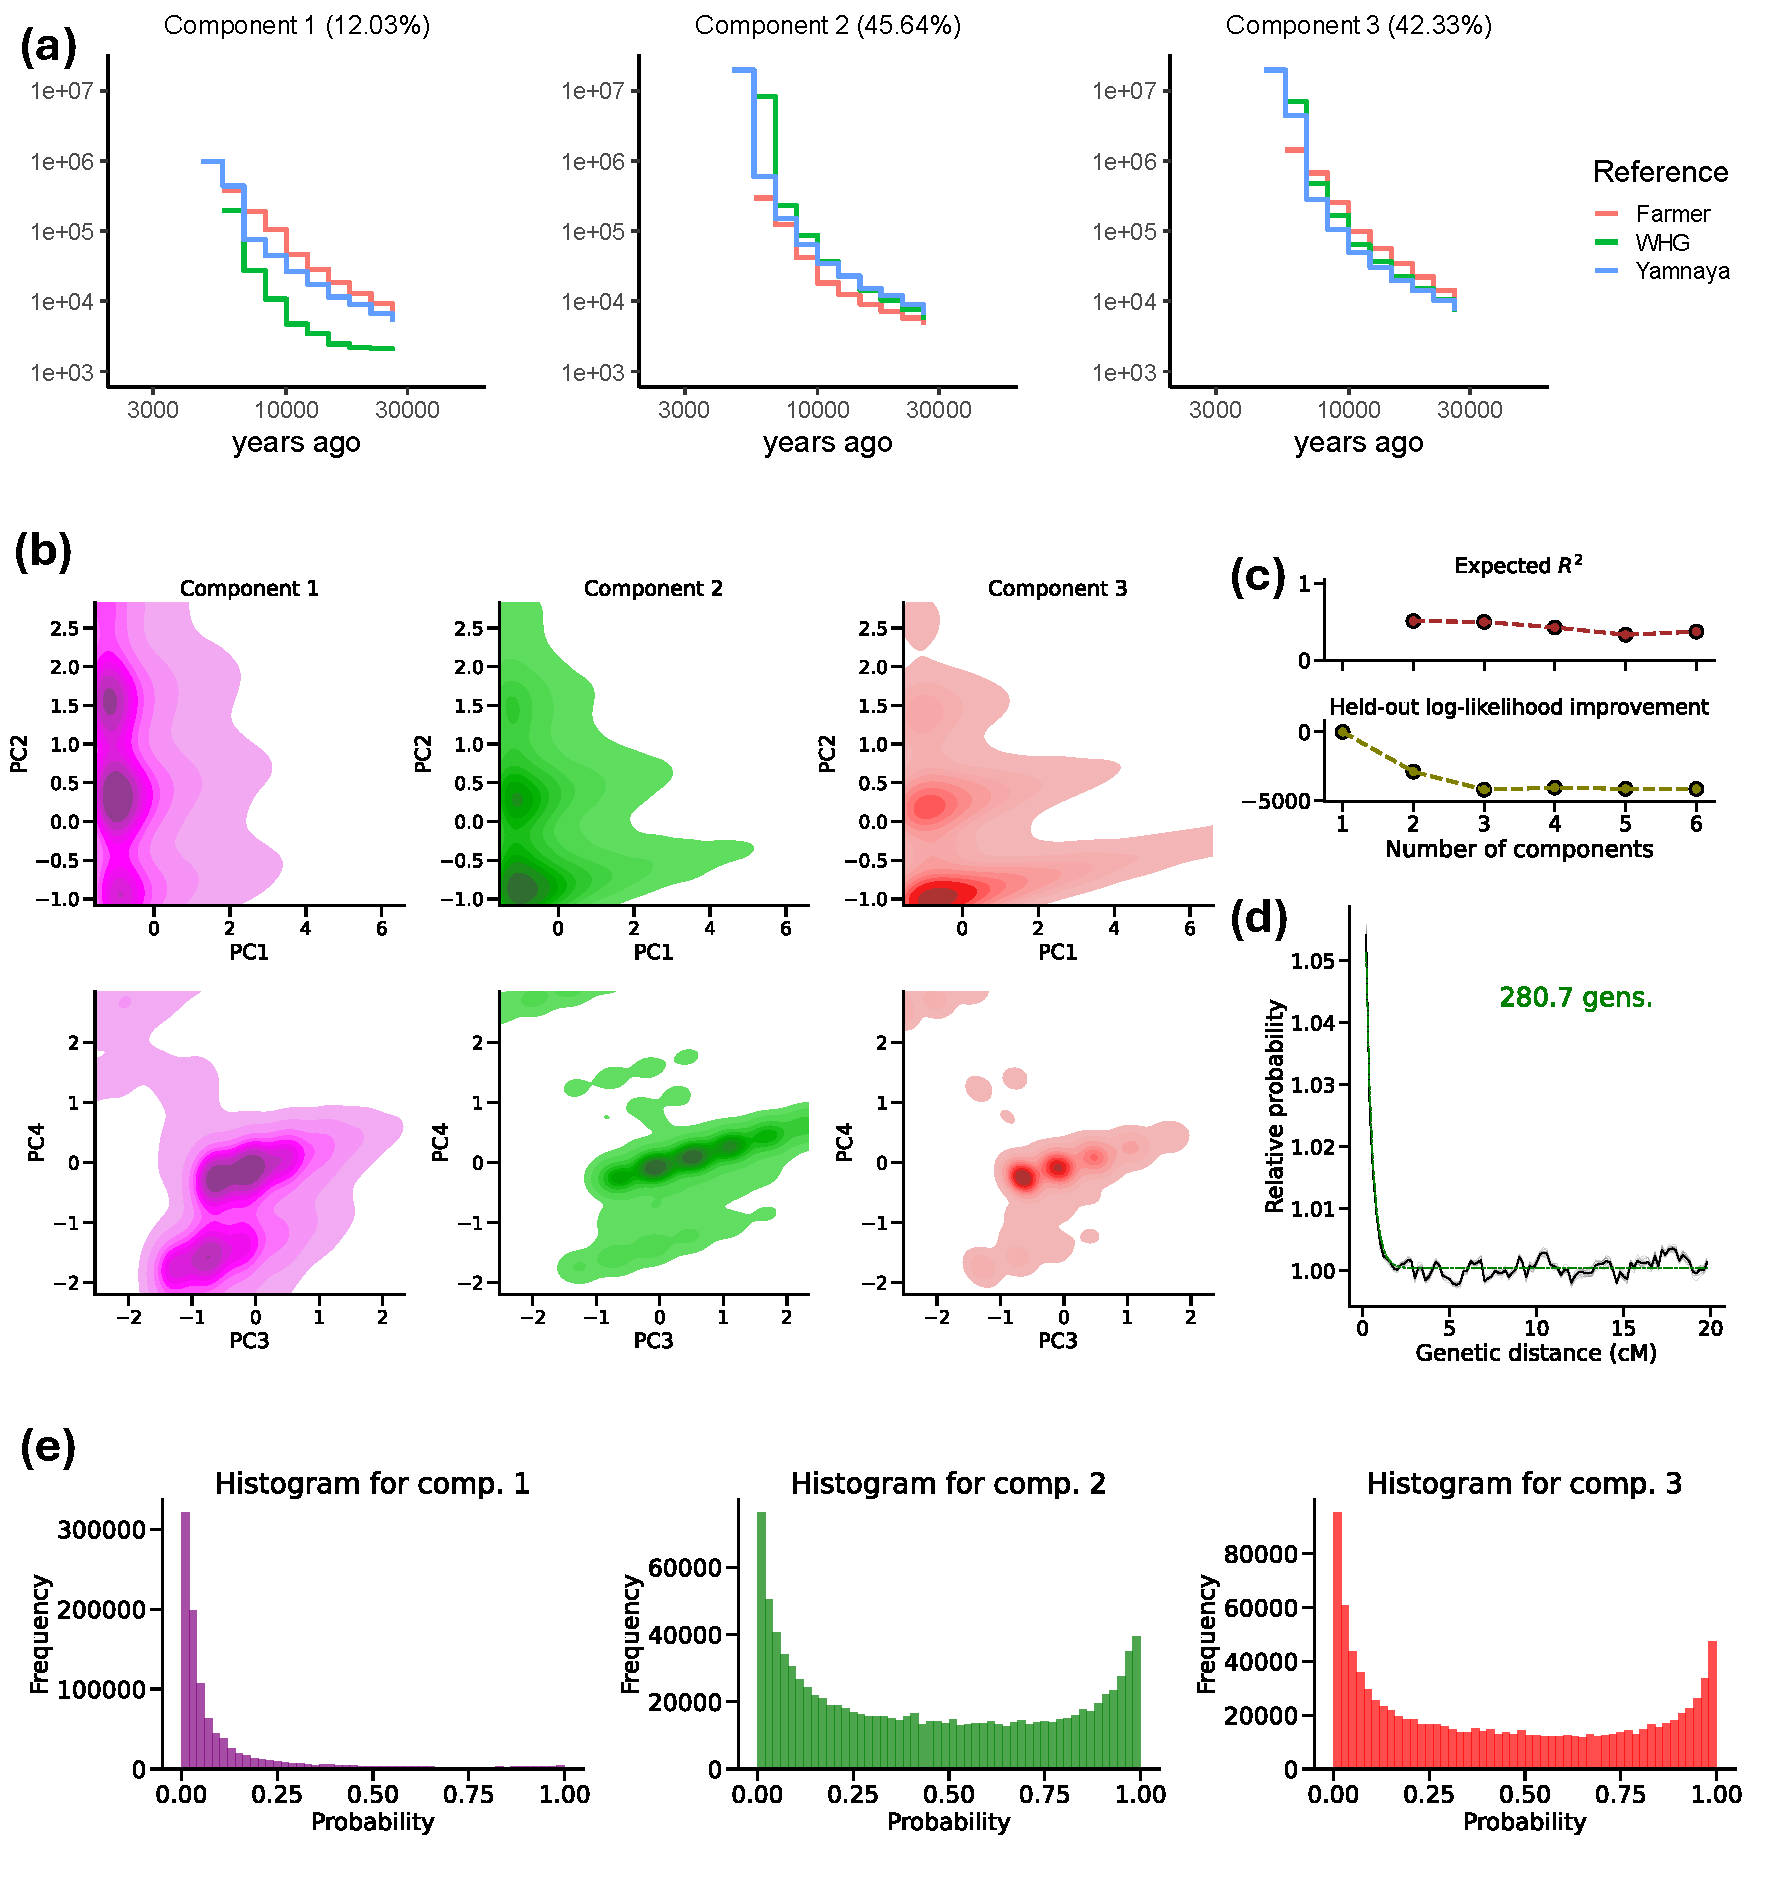
\includegraphics[width=\linewidth]{figures/gb_sims/gb_real_3way_europe.pdf}
    \captionsetup{width=\textwidth+3cm}
    \caption{
    \footnotesize
    \textbf{Decomposing British individuals in $1{,}000$GP with ancient farmers, hunter-gatherers and Yamnaya.} (a) Inferred inverse coalescence rates and proportions: each line represents inverse coalescence rate profiles with a reference population. (b) PCA visualization of the coalescence count and opportunity matrix derived from the genealogies plotted separately for each component. (c) Expected coefficient of determination and held-out log-likelihood improvement with varying number of components. (d) Coancestry curve for normalized joint probability of component 1 and the inferred admixture dates (in generations). (e) Histogram of the inferred local ancestry posteriors. The PCA visualization in (b) is based on a KDE plot with a threshold of 0.05, and binary local ancestry estimates are obtained by thresholding the inferred posteriors at 0.5.
    }
    \label{fig:gb_eur_3way}
\end{figure}

